%%%%%%%%%%%%%%%%%%%%%%%%%%%%%%%%%%%%%%%%%%%%%%%%%%%%%%%%%%%%%%%%%%%%%%
% Template for a UBC-compliant dissertation
% At the minimum, you will need to change the information found
% after the "Document meta-data"
%
%!TEX TS-program = pdflatex
%!TEX encoding = UTF-8 Unicode

%% The ubcdiss class provides several options:
%%   gpscopy (aka fogscopy)
%%       set parameters to exactly how GPS specifies
%%         * single-sided
%%         * page-numbering starts from title page
%%         * the lists of figures and tables have each entry prefixed
%%           with 'Figure' or 'Table'
%%       This can be tested by `\ifgpscopy ... \else ... \fi'
%%   10pt, 11pt, 12pt
%%       set default font size
%%   oneside, twoside
%%       whether to format for single-sided or double-sided printing
%%   balanced
%%       when double-sided, ensure page content is centred
%%       rather than slightly offset (the default)
%%   singlespacing, onehalfspacing, doublespacing
%%       set default inter-line text spacing; the ubcdiss class
%%       provides \textspacing to revert to this configured spacing
%%   draft
%%       disable more intensive processing, such as including
%%       graphics, etc.
%%

% For submission to GPS
\documentclass[gpscopy,onehalfspacing,11pt]{ubcdiss}

% For your own copies (looks nicer)
% \documentclass[balanced,twoside,11pt]{ubcdiss}

%%%%%%%%%%%%%%%%%%%%%%%%%%%%%%%%%%%%%%%%%%%%%%%%%%%%%%%%%%%%%%%%%%%%%%
%%%%%%%%%%%%%%%%%%%%%%%%%%%%%%%%%%%%%%%%%%%%%%%%%%%%%%%%%%%%%%%%%%%%%%
%%
%% FONTS:
%% 
%% The defaults below configures Times Roman for the serif font,
%% Helvetica for the sans serif font, and Courier for the
%% typewriter-style font.  Configuring fonts can be time
%% consuming; we recommend skipping to END FONTS!
%% 
%% If you're feeling brave, have lots of time, and wish to use one
%% your platform's native fonts, see the commented out bits below for
%% XeTeX/XeLaTeX.  This is not for the faint at heart. 
%% (And shouldn't you be writing? :-)
%%

%% NFSS font specification (New Font Selection Scheme)
\usepackage{times,mathptmx,courier}
\usepackage[scaled=.92]{helvet}

%% Math or theory people may want to include the handy AMS macros
\usepackage{amssymb}
\usepackage{amsmath}
\usepackage{amsfonts}

%% The pifont package provides access to the elements in the dingbat font.   
%% Use \ding{##} for a particular dingbat (see p7 of psnfss2e.pdf)
%%   Useful:
%%     51,52 different forms of a checkmark
%%     54,55,56 different forms of a cross (saltyre)
%%     172-181 are 1-10 in open circle (serif)
%%     182-191 are 1-10 black circle (serif)
%%     192-201 are 1-10 in open circle (sans serif)
%%     202-211 are 1-10 in black circle (sans serif)
%% \begin{dinglist}{##}\item... or dingautolist (which auto-increments)
%% to create a bullet list with the provided character.
\usepackage{pifont}

%%%%%%%%%%%%%%%%%%%%%%%%%%%%%%%%%%%%%%%%%%%%%%%%%%%%%%%%%%%%%%%%%%%%%%
%% Configure fonts for XeTeX / XeLaTeX using the fontspec package.
%% Be sure to check out the fontspec documentation.
%\usepackage{fontspec,xltxtra,xunicode}	% required
%\defaultfontfeatures{Mapping=tex-text}	% recommended
%% Minion Pro and Myriad Pro are shipped with some versions of
%% Adobe Reader.  Adobe representatives have commented that these
%% fonts can be used outside of Adobe Reader.
%\setromanfont[Numbers=OldStyle]{Minion Pro}
%\setsansfont[Numbers=OldStyle,Scale=MatchLowercase]{Myriad Pro}
%\setmonofont[Scale=MatchLowercase]{Andale Mono}

%% Other alternatives:
%\setromanfont[Mapping=tex-text]{Adobe Caslon}
%\setsansfont[Scale=MatchLowercase]{Gill Sans}
%\setsansfont[Scale=MatchLowercase,Mapping=tex-text]{Futura}
%\setmonofont[Scale=MatchLowercase]{Andale Mono}
%\newfontfamily{\SYM}[Scale=0.9]{Zapf Dingbats}
%% END FONTS
%%%%%%%%%%%%%%%%%%%%%%%%%%%%%%%%%%%%%%%%%%%%%%%%%%%%%%%%%%%%%%%%%%%%%%
%%%%%%%%%%%%%%%%%%%%%%%%%%%%%%%%%%%%%%%%%%%%%%%%%%%%%%%%%%%%%%%%%%%%%%



%%%%%%%%%%%%%%%%%%%%%%%%%%%%%%%%%%%%%%%%%%%%%%%%%%%%%%%%%%%%%%%%%%%%%%
%%%%%%%%%%%%%%%%%%%%%%%%%%%%%%%%%%%%%%%%%%%%%%%%%%%%%%%%%%%%%%%%%%%%%%
%%
%% Recommended packages
%%
\usepackage{checkend}	% better error messages on left-open environments
\usepackage{graphicx}	% for incorporating external images

%% booktabs: provides some special commands for typesetting tables as used
%% in excellent journals.  Ignore the examples in the Lamport book!
\usepackage{booktabs}

%% listings: useful support for including source code listings, with
%% optional special keyword formatting.  The \lstset{} causes
%% the text to be typeset in a smaller sans serif font, with
%% proportional spacing.
\usepackage{listings}
\lstset{basicstyle=\sffamily\scriptsize,showstringspaces=false,fontadjust}

%% The acronym package provides support for defining acronyms, providing
%% their expansion when first used, and building glossaries.  See the
%% example in glossary.tex and the example usage throughout the example
%% document.
%% NOTE: to use \MakeTextLowercase in the \acsfont command below,
%%   we *must* use the `nohyperlinks' option -- it causes errors with
%%   hyperref otherwise.  See Section 5.2 in the ``LaTeX 2e for Class
%%   and Package Writers Guide'' (clsguide.pdf) for details.
\usepackage[printonlyused,nohyperlinks]{acronym}
%% The ubcdiss.cls loads the `textcase' package which provides commands
%% for upper-casing and lower-casing text.  The following causes
%% the acronym package to typeset acronyms in small-caps
%% as recommended by Bringhurst.
\renewcommand{\acsfont}[1]{{\scshape \MakeTextLowercase{#1}}}

\newcommand{\abbr}[1]{\pdftooltip{\ac*{#1}{\acl{#1}}\protect{\acused{#1}}}}
\newcommand{\abbrIC}[1]{\pdftooltip{\ac*{#1}}{\acl{#1}}}

%% color: add support for expressing colour models.  Grey can be used
%% to great effect to emphasize other parts of a graphic or text.
%% For an excellent set of examples, see Tufte's "Visual Display of
%% Quantitative Information" or "Envisioning Information".
\usepackage{color}
\definecolor{greytext}{gray}{0.5}

%% comment: provides a new {comment} environment: all text inside the
%% environment is ignored.
%%   \begin{comment} ignored text ... \end{comment}
\usepackage{comment}

%% The natbib package provides more sophisticated citing commands
%% such as \citeauthor{} to provide the author names of a work,
%% \citet{} to produce an author-and-reference citation,
%% \citep{} to produce a parenthetical citation.
%% We use \citeeg{} to provide examples
\usepackage[numbers,sort&compress]{natbib}
\newcommand{\citeeg}[1]{\citep[e.g.,][]{#1}}

%% The titlesec package provides commands to vary how chapter and
%% section titles are typeset.  The following uses more compact
%% spacings above and below the title.  The titleformat that follow
%% ensure chapter/section titles are set in singlespace.
\usepackage[compact]{titlesec}
\titleformat*{\section}{\singlespacing\raggedright\bfseries\Large}
\titleformat*{\subsection}{\singlespacing\raggedright\bfseries\large}
\titleformat*{\subsubsection}{\singlespacing\raggedright\bfseries}
\titleformat*{\paragraph}{\singlespacing\raggedright\itshape}

%% The caption package provides support for varying how table and
%% figure captions are typeset.
\usepackage[format=hang,indention=-1cm,labelfont={bf},margin=1em]{caption}

%% url: for typesetting URLs and smart(er) hyphenation.
%% \url{http://...} 
\usepackage{url}
\urlstyle{sf}	% typeset urls in sans-serif


%%%%%%%%%%%%%%%%%%%%%%%%%%%%%%%%%%%%%%%%%%%%%%%%%%%%%%%%%%%%%%%%%%%%%%
%%%%%%%%%%%%%%%%%%%%%%%%%%%%%%%%%%%%%%%%%%%%%%%%%%%%%%%%%%%%%%%%%%%%%%
%%
%% Possibly useful packages: you may need to explicitly install
%% these from CTAN if they aren't part of your distribution;
%% teTeX seems to ship with a smaller base than MikTeX and MacTeX.
%%
%\usepackage{pdfpages}	% insert pages from other PDF files
%\usepackage{longtable}	% provide tables spanning multiple pages
%\usepackage{chngpage}	% support changing the page widths on demand
%\usepackage{tabularx}	% an enhanced tabular environment

%% enumitem: support pausing and resuming enumerate environments.
%\usepackage{enumitem}

%% rotating: provides two environments, sidewaystable and sidewaysfigure,
%% for typesetting tables and figures in landscape mode.  
%\usepackage{rotating}

%% subfig: provides for including subfigures within a figure,
%% and includes being able to separately reference the subfigures.
%\usepackage{subfig}

%% ragged2e: provides several new new commands \Centering, \RaggedLeft,
%% \RaggedRight and \justifying and new environments Center, FlushLeft,
%% FlushRight and justify, which set ragged text and are easily
%% configurable to allow hyphenation.
%\usepackage{ragged2e}

%% The ulem package provides a \sout{} for striking out text and
%% \xout for crossing out text.  The normalem and normalbf are
%% necessary as the package messes with the emphasis and bold fonts
%% otherwise.
%\usepackage[normalem,normalbf]{ulem}    % for \sout

%%%%%%%%%%%%%%%%%%%%%%%%%%%%%%%%%%%%%%%%%%%%%%%%%%%%%%%%%%%%%%%%%%%%%%
%% HYPERREF:
%% The hyperref package provides for embedding hyperlinks into your
%% document.  By default the table of contents, references, citations,
%% and footnotes are hyperlinked.
%%
%% Hyperref provides a very handy command for doing cross-references:
%% \autoref{}.  This is similar to \ref{} and \pageref{} except that
%% it automagically puts in the *type* of reference.  For example,
%% referencing a figure's label will put the text `Figure 3.4'.
%% And the text will be hyperlinked to the appropriate place in the
%% document.
%%
%% Generally hyperref should appear after most other packages

%% The following puts hyperlinks in very faint grey boxes.
%% The `pagebackref' causes the references in the bibliography to have
%% back-references to the citing page; `backref' puts the citing section
%% number.  See further below for other examples of using hyperref.
%% 2009/12/09: now use `linktocpage' (Jacek Kisynski): GPS now prefers
%%   that the ToC, LoF, LoT place the hyperlink on the page number,
%%   rather than the entry text.
\usepackage[bookmarks,bookmarksnumbered,%
    allbordercolors={0.8 0.8 0.8},%
    pagebackref,linktocpage%
    ]{hyperref}
%% The following change how the the back-references text is typeset in a
%% bibliography when `backref' or `pagebackref' are used
%%
%% Change \nocitations if you'd like some text shown where there
%% are no citations found (e.g., pulled in with \nocite{xxx})
\newcommand{\nocitations}{\relax}
%%\newcommand{\nocitations}{No citations}
%%
%\renewcommand*{\backref}[1]{}% necessary for backref < 1.33
\renewcommand*{\backrefsep}{,~}%
\renewcommand*{\backreftwosep}{,~}% ', and~'
\renewcommand*{\backreflastsep}{,~}% ' and~'
\renewcommand*{\backrefalt}[4]{%
\textcolor{greytext}{\ifcase #1%
\nocitations%
\or
\(\rightarrow\) page #2%
\else
\(\rightarrow\) pages #2%
\fi}}


%% The following uses most defaults, which causes hyperlinks to be
%% surrounded by colourful boxes; the colours are only visible in
%% PDFs and don't show up when printed:
%\usepackage[bookmarks,bookmarksnumbered]{hyperref}

%% The following disables the colourful boxes around hyperlinks.
%\usepackage[bookmarks,bookmarksnumbered,pdfborder={0 0 0}]{hyperref}

%% The following disables all hyperlinking, but still enabled use of
%% \autoref{}
%\usepackage[draft]{hyperref}

%% The following commands causes chapter and section references to
%% uppercase the part name.
\renewcommand{\chapterautorefname}{Chapter}
\renewcommand{\sectionautorefname}{Section}
\renewcommand{\subsectionautorefname}{Section}
\renewcommand{\subsubsectionautorefname}{Section}

%% If you have long page numbers (e.g., roman numbers in the 
%% preliminary pages for page 28 = xxviii), you might need to
%% uncomment the following and tweak the \@pnumwidth length
%% (default: 1.55em).  See the tocloft documentation at
%% http://www.ctan.org/tex-archive/macros/latex/contrib/tocloft/
% \makeatletter
% \renewcommand{\@pnumwidth}{3em}
% \makeatother

%%%%%%%%%%%%%%%%%%%%%%%%%%%%%%%%%%%%%%%%%%%%%%%%%%%%%%%%%%%%%%%%%%%%%%
%%%%%%%%%%%%%%%%%%%%%%%%%%%%%%%%%%%%%%%%%%%%%%%%%%%%%%%%%%%%%%%%%%%%%%
%%
%% Some special settings that controls how text is typeset
%%
% \raggedbottom		% pages don't have to line up nicely on the last line
% \sloppy		% be a bit more relaxed in inter-word spacing
% \clubpenalty=10000	% try harder to avoid orphans
% \widowpenalty=10000	% try harder to avoid widows
% \tolerance=1000

%% And include some of our own useful macros
% This file provides examples of some useful macros for typesetting
% dissertations.  None of the macros defined here are necessary beyond
% for the template documentation, so feel free to change, remove, and add
% your own definitions.
%
% We recommend that you define macros to separate the semantics
% of the things you write from how they are presented.  For example,
% you'll see definitions below for a macro \file{}: by using
% \file{} consistently in the text, we can change how filenames
% are typeset simply by changing the definition of \file{} in
% this file.
% 
%% The following is a directive for TeXShop to indicate the main file
%%!TEX root = diss.tex

\newcommand{\NA}{\textsc{n/a}}	% for "not applicable"
\newcommand{\eg}{e.g.,\ }	% proper form of examples (\eg a, b, c)
\newcommand{\ie}{i.e.,\ }	% proper form for that is (\ie a, b, c)
\newcommand{\etal}{\emph{et al}}

% Some useful macros for typesetting terms.
\newcommand{\file}[1]{\texttt{#1}}
\newcommand{\class}[1]{\texttt{#1}}
\newcommand{\latexpackage}[1]{\href{http://www.ctan.org/macros/latex/contrib/#1}{\texttt{#1}}}
\newcommand{\latexmiscpackage}[1]{\href{http://www.ctan.org/macros/latex/contrib/misc/#1.sty}{\texttt{#1}}}
\newcommand{\env}[1]{\texttt{#1}}
\newcommand{\BibTeX}{Bib\TeX}

% Define a command \doi{} to typeset a digital object identifier (DOI).
% Note: if the following definition raise an error, then you likely
% have an ancient version of url.sty.  Either find a more recent version
% (3.1 or later work fine) and simply copy it into this directory,  or
% comment out the following two lines and uncomment the third.
\DeclareUrlCommand\DOI{}
\newcommand{\doi}[1]{\href{http://dx.doi.org/#1}{\DOI{doi:#1}}}
%\newcommand{\doi}[1]{\href{http://dx.doi.org/#1}{doi:#1}}

% Useful macro to reference an online document with a hyperlink
% as well with the URL explicitly listed in a footnote
% #1: the URL
% #2: the anchoring text
\newcommand{\webref}[2]{\href{#1}{#2}\footnote{\url{#1}}}

% epigraph is a nice environment for typesetting quotations
\makeatletter
\newenvironment{epigraph}{%
	\begin{flushright}
	\begin{minipage}{\columnwidth-0.75in}
	\begin{flushright}
	\@ifundefined{singlespacing}{}{\singlespacing}%
    }{
	\end{flushright}
	\end{minipage}
	\end{flushright}}
\makeatother

% \FIXME{} is a useful macro for noting things needing to be changed.
% The following definition will also output a warning to the console
\newcommand{\FIXME}[1]{\typeout{**FIXME** #1}\textbf{[FIXME: #1]}}

% END


%%%%%%%%%%%%%%%%%%%%%%%%%%%%%%%%%%%%%%%%%%%%%%%%%%%%%%%%%%%%%%%%%%%%%%
%%%%%%%%%%%%%%%%%%%%%%%%%%%%%%%%%%%%%%%%%%%%%%%%%%%%%%%%%%%%%%%%%%%%%%
%%
%% Document meta-data: be sure to also change the \hypersetup information
%%

\title{Exploring the tumour microenvironment with non-invasive Magnetic Resonance Imaging techniques}
%\subtitle{If you want a subtitle}

\author{Firas Moosvi}
\previousdegree{Master of Science, University of Toronto, 2012}
\previousdegree{Bachelor of Science, University of British Columbia, 2009}

% What is this dissertation for?
\degreetitle{Doctor of Philosophy}

\institution{The University of British Columbia}
\campus{Vancouver}

\faculty{The Faculty of Science}
\department{Physics \& Astronomy}
\submissionmonth{November}
\submissionyear{2018}

%% hyperref package provides support for embedding meta-data in .PDF
%% files
\hypersetup{
  pdftitle={Exploring the tumour microenvironment with non-invasive Magnetic Resonance Imaging techniques (DRAFT: \today)},
  pdfauthor={Firas Moosvi},
  pdfkeywords={MRI, Cancer, tumours, CEST, HPG, contrast agents, oxygen enhanced MRI}
}

%%%%%%%%%%%%%%%%%%%%%%%%%%%%%%%%%%%%%%%%%%%%%%%%%%%%%%%%%%%%%%%%%%%%%%
%%%%%%%%%%%%%%%%%%%%%%%%%%%%%%%%%%%%%%%%%%%%%%%%%%%%%%%%%%%%%%%%%%%%%%
%% 
%% The document content
%%

%% LaTeX's \includeonly commands causes any uses of \include{} to only
%% include files that are in the list.  This is helpful to produce
%% subsets of your thesis (e.g., for committee members who want to see
%% the dissertation chapter by chapter).  It also saves time by 
%% avoiding reprocessing the entire file.
%\includeonly{intro,conclusions}
%\includeonly{discussion}

\begin{document}

%%%%%%%%%%%%%%%%%%%%%%%%%%%%%%%%%%%%%%%%%%%%%%%%%%
%% From Thesis Components: Tradtional Thesis
%% <http://www.grad.ubc.ca/current-students/dissertation-thesis-preparation/order-components>

% Preliminary Pages (numbered in lower case Roman numerals)
%    1. Title page (mandatory)
\maketitle

%    2. Abstract (mandatory - maximum 350 words)
%% The following is a directive for TeXShop to indicate the main file
%%!TEX root = diss.tex

\chapter{Abstract}

This thesis comprises development and application of several MRI techniques to improve our understanding of tumour growth, drug distribution, and drug effect using pre-clinical tumour models in mice. In the first part of the thesis, a novel high molecular weight contrast agent, HPG-GdF is introduced. This molecule is a hyperbranched polyglycerol labeled with an MRI contrast agent (Gd-DOTA) as well as a fluorescent tag. After injecting the agent into mice within an MRI scanner, contrast-agent kinetics were quantified using a two-parameter linear model and validated with quantitative immunohistochemistry via direct fluorescence imaging of HPG-GdF.

HPG-GdF was used to assess whether vascular function plays a role in how a chemotherapy (Herceptin) distributes within a tumour. Tumour vessel permeability and fractional plasma volume were quantified using the HPG-GdF and no relationship was found between vascular function and presence of drug. HPG-GdF was then applied to show that Avastin (an antiangiogenic agent) decreased vessel permeability in tumours. Using histological methods, a dramatic reduction in hypoxia (oxygen deficiency in tissues) was observed in treated tumours. Unfortunately, existing MRI methods to evaluate oxygenation were time-intensive and lacked sensitivity. In the second part of this thesis, we introduce, develop, validate, and apply a new method to assess tumour oxygenation using MRI. 

Oxygen (O$_2$) is a paramagnetic molecule that shortens the longitudinal relaxation time (T$_1$) of protons in MRI. This subtle effect has been widely reported in the literature but its applications in cancer have been limited. Our technique - dynamic oxygen-enhanced MRI (\acs{dOE-MRI}) - uses T$_1$W signal intensity images acquired during a cycling gas challenge (air or oxygen) and independent component analysis (ICA). Hypoxia staining with pimonidazole correlated strongly with \acs{dOE-MRI} values in a murine tumour model (SCCVII) and only weakly in a colorectal xenograft model (HCT-116). Finally, we provide compelling evidence that treatment with Avastin improves tumour oxygenation in subcutaneous tumours. With \acs{dOE-MRI}, the sensitivity and speed of existing techniques was greatly improved. Since our technique requires no injectable contrast agent, special sequences or hardware, we anticipate that this technique can be quickly translated into the clinic. 


% Consider placing version information if you circulate multiple drafts
\vfill
\begin{center}
\begin{sf}
\fbox{Git commit: d81f849}
\end{sf}
\end{center}

\cleardoublepage

%    3. Lay Summary (Effective May 2017, mandatory - maximum 150 words)
%% The following is a directive for TeXShop to indicate the main file
%%!TEX root = diss.tex

%% https://www.grad.ubc.ca/current-students/dissertation-thesis-preparation/preliminary-pages
%% 
%% LAY SUMMARY Effective May 2017, all theses and dissertations must
%% include a lay summary.  The lay or public summary explains the key
%% goals and contributions of the research/scholarly work in terms that
%% can be understood by the general public. It must not exceed 150
%% words in length.

\chapter{Lay Summary}

In this thesis we have described the development and application of several magnetic resonance imaging (MRI) techniques to improve our understanding of tumour in mice.
In the first part of the thesis, a new analysis method was outlined to characterize tumour blood vessels with a novel bio-compatible contrast agent.
In the second part of this thesis, we introduced, developed, validated, and applied a new method to assess tumour oxygenation using MRI.
Our technique is a significant improvement over other available methods as it uses a machine learning technique to extract very small changes in MRI signal just by inhaling 100\% oxygen gas. 
We used this technique to show that treatment with a cancer drug that prunes malformed and abnormal blood vessels in tumour improves oxygenation levels.
Since our technique requires no injectable contrast agent, special sequences or hardware, we anticipate that this technique can be quickly translated into the clinic. 

\cleardoublepage

%    4. Preface
%% The following is a directive for TeXShop to indicate the main file
%%!TEX root = diss.tex

\chapter{Preface}

At \ac{UBC}, a preface may be required.  Be sure to check the
\ac{GPS} guidelines as they may have specific content to be included.

\cleardoublepage

%    5. Table of contents (mandatory - list all items in the preliminary pages
%    starting with the abstract, followed by chapter headings and
%    subheadings, bibliographies and appendices)
\tableofcontents
\cleardoublepage	% required by tocloft package

%    6. List of tables (mandatory if thesis has tables)
\listoftables
\cleardoublepage	% required by tocloft package

%    7. List of figures (mandatory if thesis has figures)
\listoffigures
\cleardoublepage	% required by tocloft package

%    8. List of illustrations (mandatory if thesis has illustrations)
%    9. Lists of symbols, abbreviations or other (optional)

%   10. Glossary (optional)
%% The following is a directive for TeXShop to indicate the main file
%%!TEX root = diss.tex

\chapter{Glossary}

% use \acrodef to define an acronym, but no listing
\acrodef{UI}{user interface}
\acrodef{UBC}{University of British Columbia}

\acrodef{DCE-US}{dynamic contrast enhanced ultrasound}
\acrodef{ICA}{Independent Component Analysis}


% The acronym environment will typeset only those acronyms that were
% *actually used* in the course of the document
\begin{acronym}

\acro{ICA}[ICA]{Independent Component Analysis; a blind source separation technique that splits a multi-source signal into its constituents}

\acro{dOE-MRI}[dOE-MRI]{dynamic Oxygen Enhanced MRI; a technique that relies on the T$_1$-shortening property of oxygen and independent component analysis to identify regions that respond to an oxygen stimulus.}

\acro{DCE-US}[DCE-US]{dynamic contrast enhanced ultrasound; an imaging technique that uses echogenic microbubbles to enhance contrast \emph{in vivo}.}

\acro{CD31}[CD31]{cluster of differentiation 31 (CD31), also known as platelet endothelial cell adhesion molecule (PECAM) is a protein that is used in immunohistochemistry primarily to demonstrate the presence of endothelial cells.}

\acro{Hoechst 33342}[bisbenzimide]{Hoechst 33342 (also known as bisbenzimide) is an organic compound used as a fluorescent stain for DNA}

\acro{EPR}[EPR]{EPR, or enhanced permeability and retention is a phenomenon that results in macromolecules are retained in the tumour and extravasation into the tumour interstitium continues due to poor lymphatic clearance and other factors.}

\acro{CA}[CA]{Contrast agent}

\acro{MCA}[MCA]{Macromolecular contrast agents.}

\acro{aPS}[aPS]{Apparent permeability surface area product; a parameter derived from DCE-MRI using HPG}

\acro{fPV}[fPV]{Fractional plasma volume}

\acro{HPG-GdF}[HPG-GdF]{Hyperbranched polyglycerol (HPG) chelated to Gd-DTPA with a fluorophore (F) attached; 500 kDa) }

\acro{MW}[MW]{Molcular weight}

\acro{MAb}[MAb]{Monoclonal antibody}
\acroplural{MAbs}[MAbs]{Monoclonal antibodies}
\acro{}[]{}
\acro{}[]{}
\acro{}[]{}
\acro{}[]{}
\acro{}[]{}
\acro{}[]{}



\end{acronym}

% You can also use \newacro{}{} to only define acronyms
% but without explictly creating a glossary
% 
% \newacro{ANOVA}[ANOVA]{Analysis of Variance\acroextra{, a set of
%   statistical techniques to identify sources of variability between groups.}}
% \newacro{API}[API]{application programming interface}
% \newacro{GOMS}[GOMS]{Goals, Operators, Methods, and Selection\acroextra{,
%   a framework for usability analysis.}}
% \newacro{TLX}[TLX]{Task Load Index\acroextra{, an instrument for gauging
%   the subjective mental workload experienced by a human in performing
%   a task.}}
% \newacro{UI}[UI]{user interface}
% \newacro{UML}[UML]{Unified Modelling Language}
% \newacro{W3C}[W3C]{World Wide Web Consortium}
% \newacro{XML}[XML]{Extensible Markup Language}
	% always input, since other macros may rely on it

\textspacing		% begin one-half or double spacing

%   11. Acknowledgements (optional)
%% The following is a directive for TeXShop to indicate the main file
%%!TEX root = diss.tex

\chapter{Acknowledgments}

This work would not be possible without the tireless commitment and mentoring by my supervisor, Dr. Stefan Reinsberg.
Dr. Baker was also instrumental in helping run, plan, and provide support for all of the work presented here. 
Members of my supervisory committee, Drs. Kozlowski, Laule, and Minchinton were excellent sources of advice, feedback, guidance, and general project direction. 
Particular thanks to Dr. Kozlowski for supporting and organizing weekly lab meetings giving me and other trainees to give and get honest feedback on preliminary work - I learned a tonne through these meetings.

Finally, a huge thanks goes to my family, and my wife who has supported and humoured me through my meanderings over the course of my PhD. 

%   12. Dedication (optional)

% Body of Thesis (not all sections may apply)
\mainmatter

\acresetall	% reset all acronyms used so far

%    1. Introduction
%% The following is a directive for TeXShop to indicate the main file
%%!TEX root =../diss.tex

\chapter{Introduction}
\label{ch:Introduction}

\section{Cancer}

Some facts about prevalence of cancer and poor outcomes, high toxicity to motivate this work.\todo[backgroundcolor=red!20!white]{to fix}

\todo[backgroundcolor=red!20!white]{this section needs a thorough re-write i think}
\subsection{Current therapies}
\todo[backgroundcolor=red!20!white]{Change title to less broad (from SAR)}
Numerous advancements in chemotherapies over the past decade have sparked an urgent clinical need for non-invasive methods to assess treatment efficacy.
There is a knowledge gap in the use and synergistic combinations of therapies, and many treatment regimens expose patients to higher toxicity than necessary.
Despite known extremes in patient response to treatment - even in cancers of the same type and grade - doses are generally prescribed by success rates of trials in patient populations exhibiting similar disease manifestations.
Each class of drugs has unique modes of action and still, there are no reliable and reproducible methods to assess synergistic benefits of combined therapy regimens~\cite{Zhang:2008ie}.
Traditionally, a prominent measure of treatment response has been to track tumour shrinkage following treatment~\cite{Tuma:2006hx}.
However, it has been shown that tumour shrinkage can take weeks and sometimes even months to manifest~\cite{Brindle:2008jt} and in some cases may not occur at all~\cite{Kitzen:2008un}.
For instance, anti-angiogenic agents typically arrest tumour growth by disrupting existing vasculature or inhibiting new vessel growth.
Despite positive effect, these agents may not necessarily lead to tumour shrinkage.
This mode of drug action is better characterized by assessing tumour vascular function rather than gross changes in physical size.
Development of quantitative and non-invasive methods to assess tumours following therapy continues to be a burgeoning field.
Furthermore, there is an urgent need in the drug development and testing community as drugs that fail in the late stages of clinical trials have led to an astronomical rise in the cost of developing drugs.
Lack of effective patient stratification techniques to identify potential responders from non-responders is a key reason that drugs fail.
For instance clinical trials targeting hypoxia - a key target for both chemotherapy to improve drug delivery and radiotherapy to increase radiosensitivity - have been conducted without patient selection or stratification based on pre-treatment tumour hypoxia status and therefore include patients with different hypoxic fractions~\cite{Overgaard:2011ji}.
This is at least partially due to an absence of validated methods that can accurately assess the hypoxia status of tumours \emph{in vivo}.
The benefits of developing early, non-invasive measures of treatment efficacy are clear for both patients and health care systems.
For patients, if a standard treatment regimen is prescribed and deemed ineffective early, the treatment can be altered and patients can directly benefit from personalized care.
Similarly, with improved patient stratification using non-invasive gross assessments of the tumour status, these patients can avoid receiving ineffective and expensive therapies.
However, the choice of appropriate biomarkers for many targets remains elusive. 

\subsection{Cancer Biomarkers and targets} There has been considerable interest in predictive biomarkers for early assessment.
Several candidates have appeared and disappeared but in 2000, a seminal paper catalogued a vast array of cancer cell genotypes into ``six essential alterations in cell physiology that collectively dictate malignant growth in tumours''~\cite{Hanahan:2000wo} (figure~\ref{cancerHallmarks}): 1) self-sufficiency in growth signals, 2) insensitivity to growth-inhibitory signals, 3) evasion of programmed cell death, 4) limitless replicative potential, 5) sustained angiogenesis and, 6) tissue invasion and metastasis~\cite{Hanahan:2000wo}.
In 2011, taking into account the progress made over a decade, the framework expanded to inculde four more hallmarks for the next generation~\cite{Hanahan:2011gu}.
Angiogenesis, the 5th hallmark is particularly suitable for consideration in non-invasive imaging techniques, particularly MRI. 

\begin{figure}[htbp]   
 \begin{center}  
 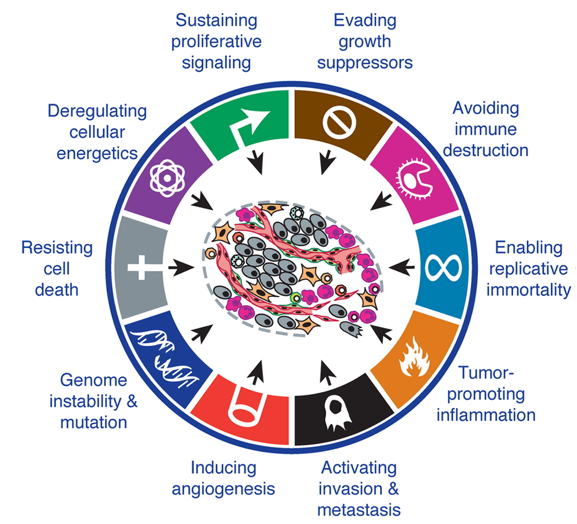
\includegraphics[width=4in]{intro/./intro-images/cancerHallmarks.png}
 \caption{Graphical illustration of the hallmarks of cancer; many of these targets are inaccessible to non-invasive imaging. Figure from the Hanahan group~\cite{Hanahan:2011gu}.}  
 \label{cancerHallmarks}  
 \end{center}
\end{figure}

Angiogenesis, or the formation of new blood vessels from pre-existing ones is a normal and vital process in the body tightly regulated by various cell signalling pathways and growth factors.
In tumours, angiogenesis is a critical step in the growth and spread of tumours as new blood vessels are recruited from the existing vascular network to promote rapidly accelerated and abnormal tumour growth~\cite{Folkman:1990ud}.
Normally, this process is regulated by several angiogenic and antiangiogenic factors such as $\alpha \beta$ integrin, vascular endothelial growth factor (VEGF) and fibroblast growth factor~\cite{Laking:2006ij}.
In tumours however, this process is completely deregulated (figure~\ref{tumourVasculature}) and excess production of growth factors from rapidly proliferating tumour cells leads to a drastic increase in vasculogenesis.
These newly formed vessels are unstable and must mature with the addition of pericytes, cells that surround the endothelium providing structural support.
Pericytes are often malformed and poorly distributed in solid tumours contributing to a dysfunctional vascular network.
Vessel growth patterns in tumours are generally accepted to be abnormal with a defective and leaky endothelium~\cite{McDonald:2002ut}.
Irregular diameters of tumour vessels, abnormal branching patterns and leaky vessel walls all contribute to an increase in vessel permeability.
It is estimated that a single hole larger than 0.5$\mu$m in diameter would alter the permeability of that vessel significantly enough to result in solute extravasation to be limited by blood flow~\cite{McDonald:2002ut}.
Disorganized and inefficient blood flow also limits the delivery of macromolecules, such as chemotherapeutic agents via the blood.
Poor perfusion in the tumour due to a disorganized vascular network impairs the delivery of systemic drugs to the whole tumour and ultimately, reduces efficacy. 

%\begin{wrapfigure}{L}{0.65\textwidth} 
\begin{figure}  
 \begin{center}  
 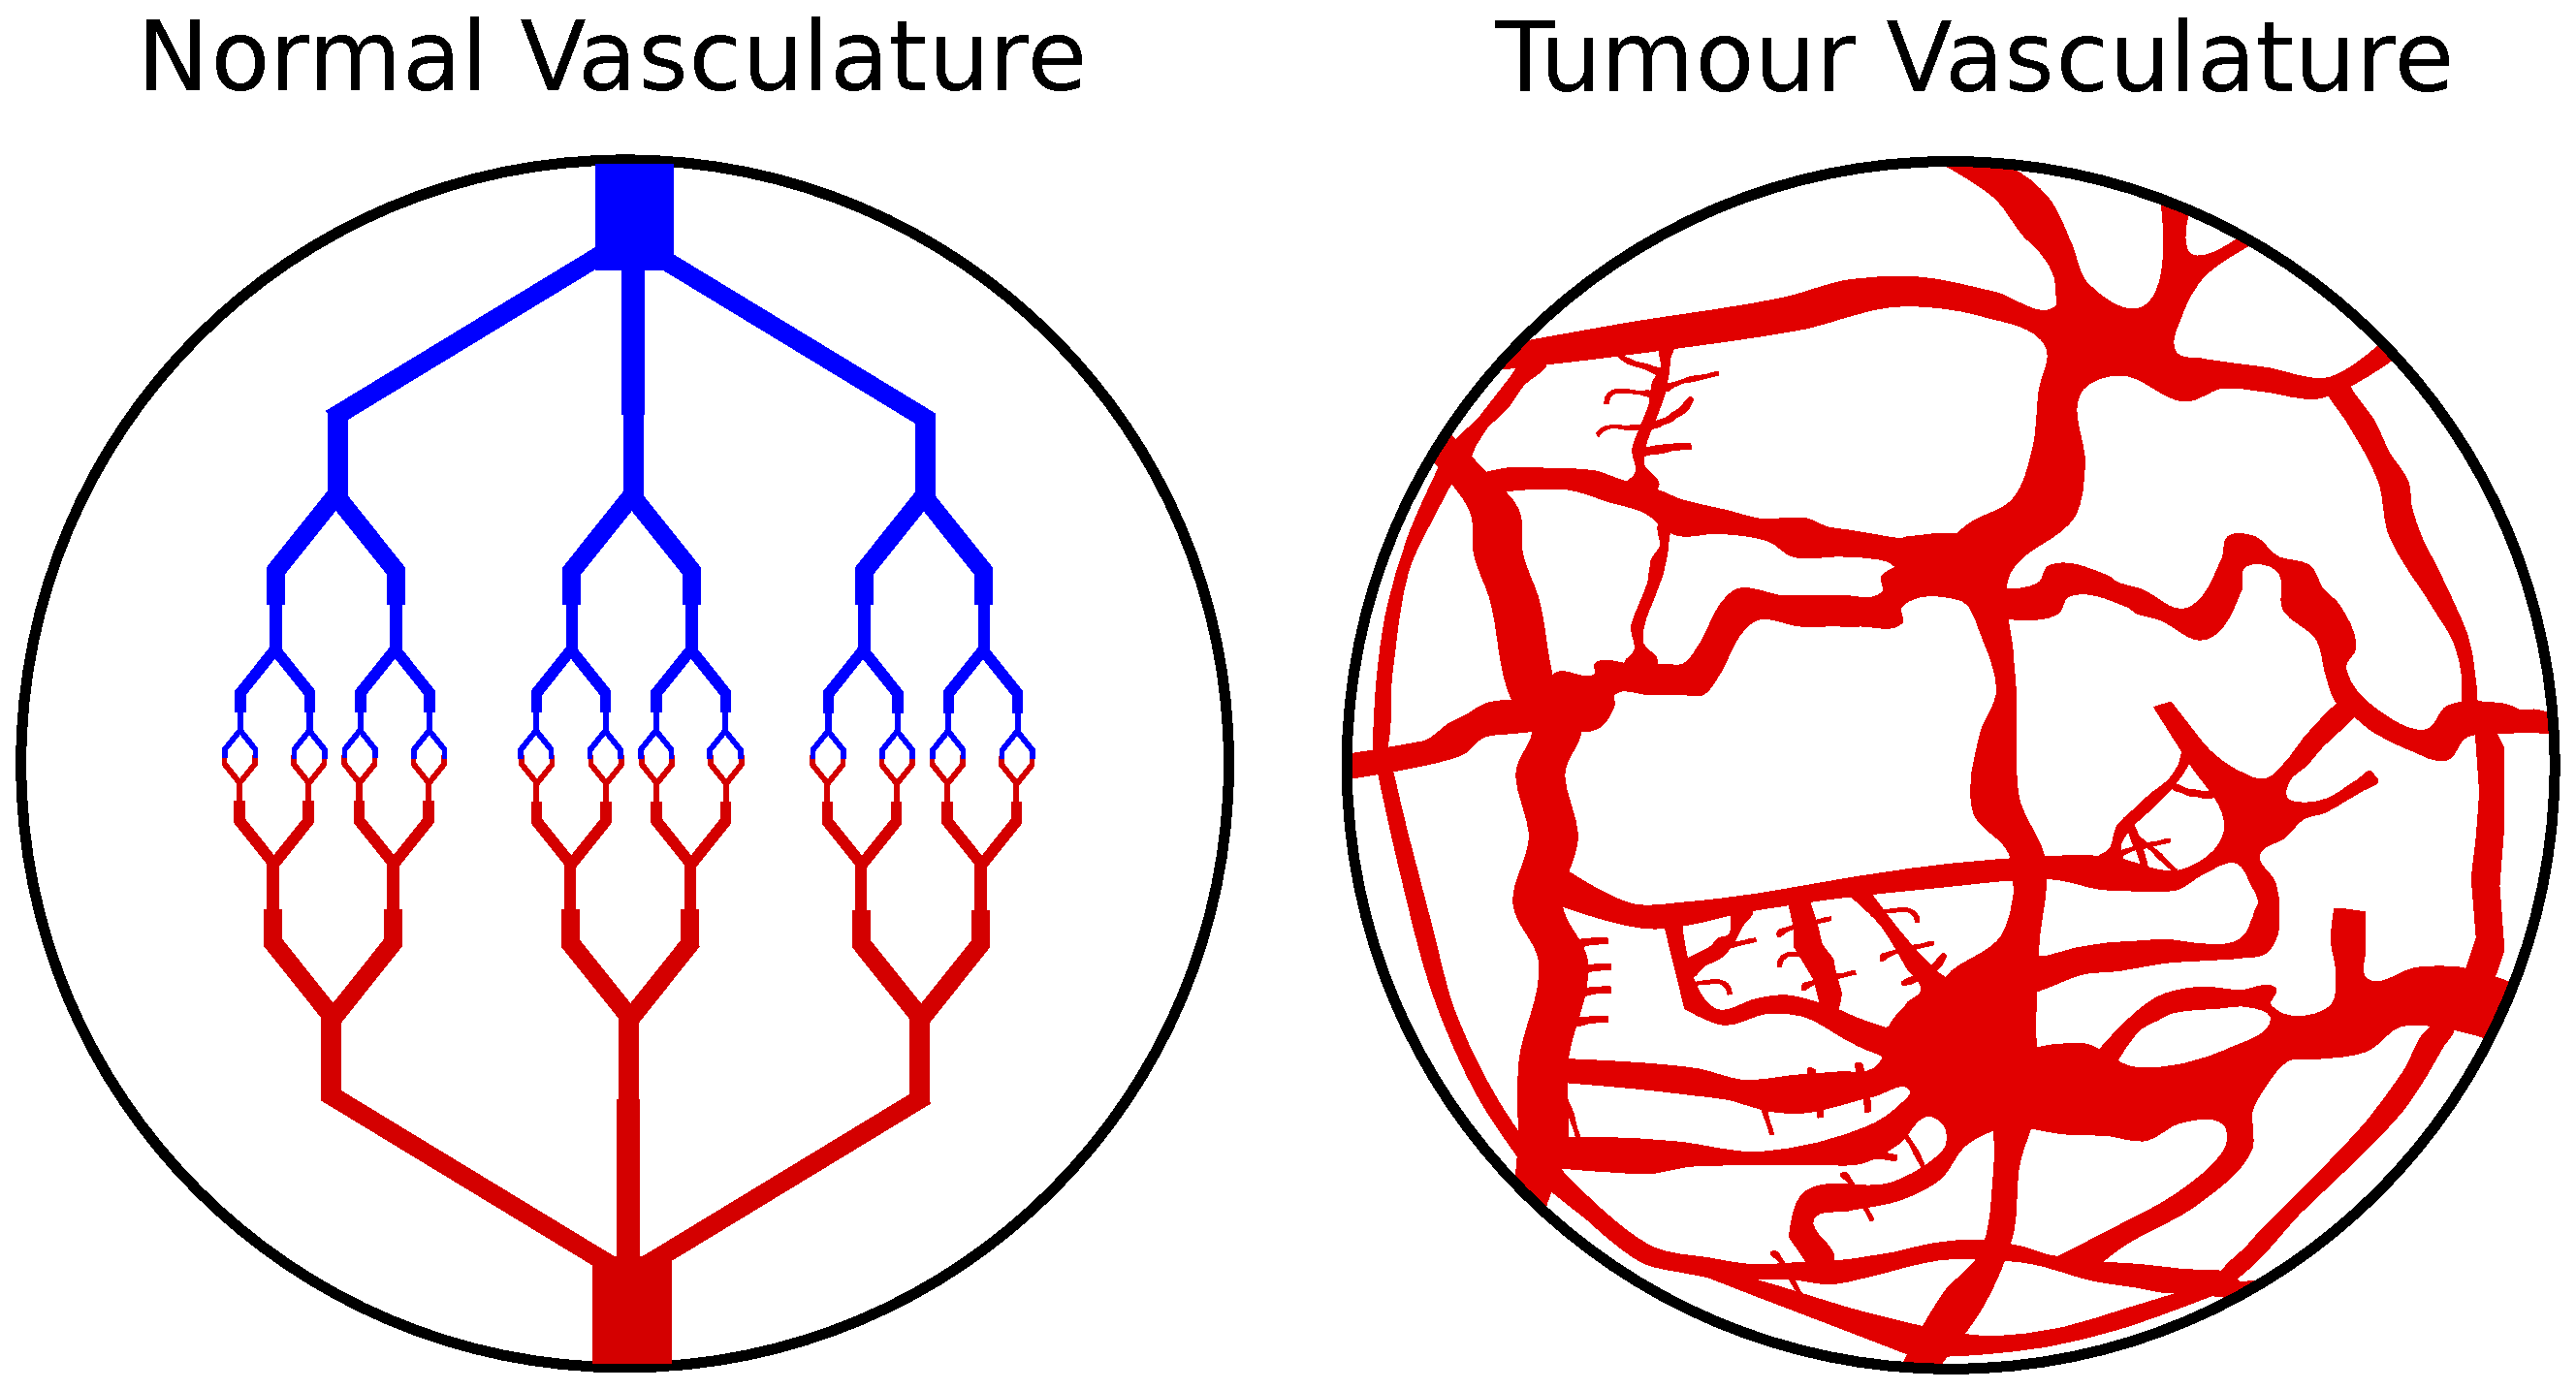
\includegraphics[width=4in]{intro/intro-images/tumourVasculature.pdf}
 \caption{Schematic of the normal tissue (left) and tumour (right) vasculature network. 
 Note the hierarchical structure of oxygenated blood (red) passing through the arteries, arterioles, and deoxygenated blood leaving via the venules, veins. 
 In tumours, this structure is severely compromised and often, no clear flow patterns can be distinguished with many vessels ending in dead ends or looping back onto feeding vessels.}
 \label{tumourVasculature}
 \end{center}
\end{figure}

Several strategies have been proposed to maximize cell kill, including the combination of different therapies (such as radiotherapy and chemotherapy) and agents that ``normalize'' the tumour vasculature and prime them for receiving chemotherapies~\cite{Jain:2005gk}.
Tumour angiogenesis is extremely important in tumour growth, progression and metastasis and is a promising target for novel therapies~\cite{Miles:2000wq}.
For instance, ``measuring'' tumour angiogenesis has the potential to serve as a highly predictive prognostic marker for disease outcome and treatment.
Histology remains the gold standard for angiogenesis detection (microvessel density) but has several critical limitations.
Histology requires biopsy samples and patient comfort aside, biopsies only sample a small fraction of the potentially affected organ.
The lack of functional information from biopsies as well as the practical challenges of obtaining longitudinal biopsy samples make non-invasive imaging a promising technique to complement and potentially reduce unneeded biopsies.

\subsection{Need for non-invasive imaging}
Non-invasive imaging methods are proving indispensable for studying angiogenesis \emph{in vivo} as they provide researchers with quantitative information about blood flow, vascular permeability, vessel density, vessel function and blood volume~\cite{McDonald:2003cm}.
Imaging modalities such as computed tomography (CT), magnetic resonance imaging (MRI), positron emission tomography (PET), single photon emission computed tomography (SPECT) and ultrasound (US), have all been proposed for studying angiogenesis~\cite{Laking:2006ij}.
Each modality is optimal for probing a particular aspect of biomarkers. To study angiogenesis and its effects on tumour growth and treatment response, the tumour environment needs to be probed using tools that assess both the interstitial tumour volume as well as the tumour vasculature.
Nuclear medicine techniques such as PET and SPECT employ radiotracers that can be measured at picomolar concentrations but at a significantly lower spatial resolution.
DCE-MRI and DCE-CT offer similar perfusion measurements (rate of leakage and leakage space) as both rely on the administration of a contrast agent that diffuses from the vasculature.
DCE-CT is advantageous as it has a direct linear relationship between the contrast agent concentration and the image intensity (attenuation numbers, given by Houndsfield Units)~\cite{Cuenod:2006jy}.
The disadvantage of CT however is that it requires ionizing radiation and iodinated contrast agents used in CT have been shown to have lower safety profiles compared to MR contrast agents~\cite{Hasebroock:2009hw}.
MRI can also be used to measure additional information such as diffusion, tissue oxygenation, spectroscopy, chemical exchange and magnetization transfer. 
In this thesis, several techniques will be explored in a bid to improve our understanding of the tumour microenvironment.

\section{Magnetic Resonance Imaging}

In biological specimens, water is by far the most abundant molecule in the body and the hydrogen atom in water is central to MR imaging.
Other MR-active atoms include $^{13}$C, $^{19}$F, $^{23}$Na and $^{31}$P, but these are rare and not used in this thesis.
We begin our description of the principles of magnetic resonance imaging, outside the scanner in a bucket of water.
The molecular mass of a water molecule (H$_2$O) is approximately 18 g/mol and its density is 1 g/mL so in this 1L bucket, there are approximately 3$\times10^{25}$ molecules of water.
Moving from macroscopic to microscopic, each molecule of water contains two hydrogen atoms and one oxygen atom.
Within the nucleus of a hydrogen atom, there is a single proton, resulting in a net positive charge on the atom.
An intrinsic property of fundamental particles such as the proton and neutron is that they posses spin angular momentum.
Incidentally, spin is the only quantum mechanics required to understand the vast majority of MR principles~\cite{Hanson:2008tp}.
Nuclei ``inherit'' this quantum mechanical property from its constituent subatomic particles - in particular, neutrons and protons.
The nucleus of a hydrogen atom has an odd number of protons (n=1) so there is a net spin angular momentum.
This results in the nucleus having an intrinsic magnetic moment arising from the net nuclear spin angular momentum and net charge from the proton.
Though there is no analogy to this from a classical physics perspective, one can imagine the net magnetic moment of a proton as a close cousin to the classical situation of the magnetic field generated by a loop of current in a wire.
To summarize, each proton in the hydrogen nucleus has spin angular momentum, is charged and thus has a net magnetic moment.

We will model the hydrogen atom with a net magnetic moment as a small bar magnet spinning on its own axis (with an arrow vector representing the direction and strength of the magnetic moment) and rely on classical physics to describe the principle of magnetic resonance imaging. 
If a spinning bar magnet is placed in an external magnetic field, the magnetic moment vector of the bar magnet will precess, or rotate about the new magnetic field with a frequency known as the Larmor frequency:

\begin{equation}
	\omega = \gamma \vec{\mathbf{B_0}}
\end{equation}

The proportionality factor $\gamma$ is the gyromagnetic ratio and is nuclei-dependent and for protons, $\gamma = 42 MhZ /T$.
For convenience it is useful to change our reference frame to a rotating reference frame so the the magnetic moment vector is stationary on a (rotating) cartesian axis.
\todo[backgroundcolor=red!20!white]{add caption to this figure}
\begin{figure}
	\centering
	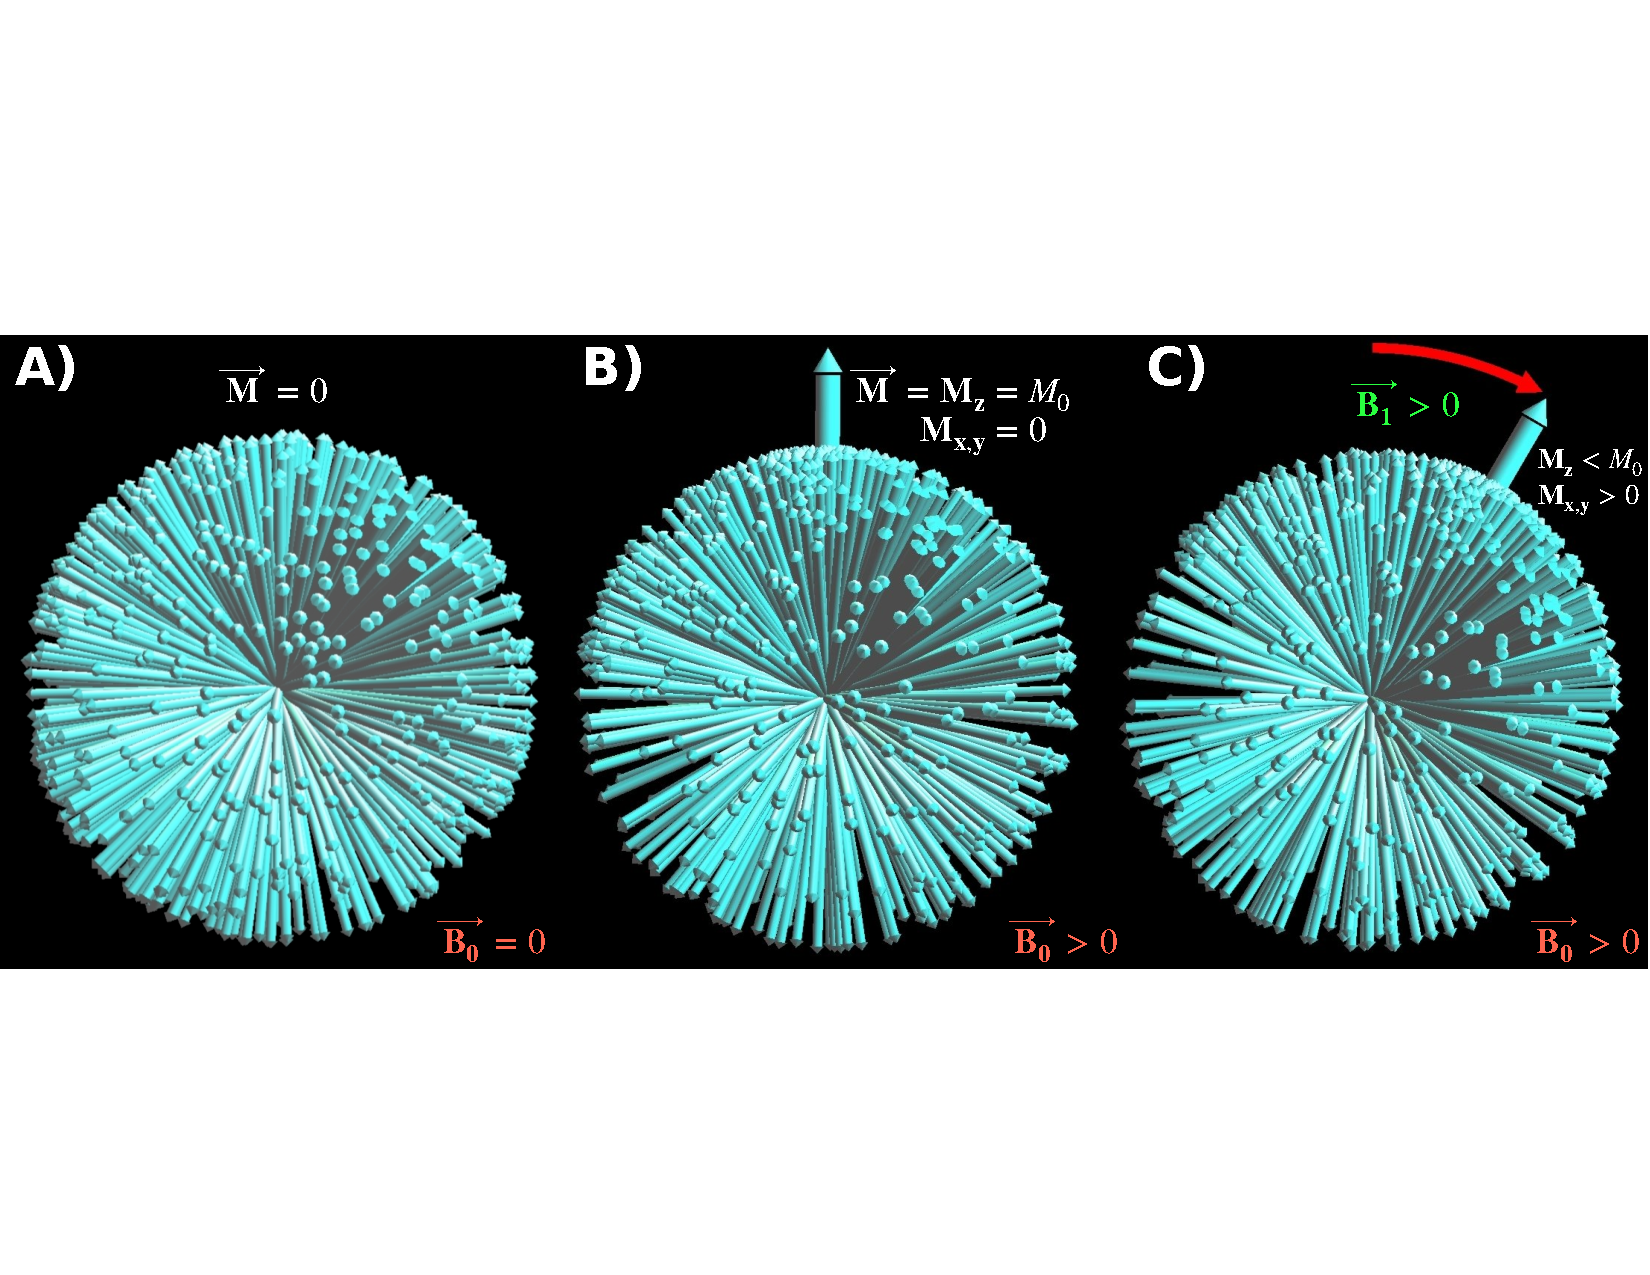
\includegraphics[width=\textwidth]{./intro/intro-images/HansonMRI.pdf}
	\caption[Spins getting tipped with an RF pulse]{The net magnetization vector M$_0$ is tipped to the transverse axis with an RF pulse so the signal can be measured. 
Images used with permission from Hanson et al. 
(\cite{Hanson:2008tp})}
	\label{spinsB0B1}
\end{figure}

Back to the bucket of water, or rather, a collection of many many small bar magnets.
Rather than consider 1$0^{25}$ bar magnets, it is simpler to consider the net magnetic moment of all the protons in aggregate.
This vector is typically referred to as the magnetization vector $\vec{\mathbf{M}}$ and comprises MRI signal and its manipulation and interactions with the surrounding environment ultimately lead to the images produced.
Because the magnets are tumbling around in the bucket of water due to thermal motion, they are pointed in nearly every direction (figure~\ref{spinsB0B1}A) and $\vec{\mathbf{M}} = 0$.
If we now put this bucket of water into an MRI scanner with a main magnetic field strength $\vec{\mathbf{B_0}} = 7$ Tesla, there is a slight tendency of individual protons to align with the main magnetic field $\vec{\mathbf{B}}$ (along z axis, see figure~\ref{spinsB0B1}B).
Consequently the magnetization vector $\vec{\mathbf{M}}$ now aligns with $\vec{\mathbf{B_0}}$.
If $\vec{\mathbf{M}}$ is split into its components (along the x, y, and z axes), the longitudinal magnetization component $\mathbf{M_z} = M_0$ and the transverse magnetization component $\mathbf{M_{x,y}} = 0$.
$\vec{\mathbf{M}}$ is many orders of magnitude smaller than the external magnetic field so the MR signal cannot be measured when it is aligned with the external main magnetic field $\vec{\mathbf{B}}$. 
Applying a radiofrequency (RF) pulse $\vec{\mathbf{B_1}}$ at the Larmor frequency results in a torque applied to $\vec{\mathbf{M}}$, causing it to `tip' down into the transverse (x-y) plane (figure~\ref{spinsB0B1}C)

In the transverse plane, interacting nuclei exchange energy with both the surrounding environment (spin-lattice interaction) as well as neighbouring nuclei (spin-spin interaction), and $\vec{\mathbf{M}}$ relaxes back to its equilibrium value. 
The time it takes for $\mathbf{M_z}$ to return to its equilibrium value $\vec{\mathbf{M_0}}$ from 0, is characterized by the time T$_1$,

\begin{equation}
	M_z = M_z(1-e^{-t/T_1})
	\label{T1}
\end{equation}

Similarly, the transverse magnetization $\mathbf{M_{x,y}}$ decays to 0 through the interactions between nuclei and is characterized by the time T$_2$ (also called spin-spin relaxation).
		
\begin{equation}
		M_{xy} = M_0 e^{-t/T_2}
		\label{T2}
\end{equation}

Although T$_1$ and T$_2$ values are affected by various factors including field-strength, and local environmental factors such as temperature, proton concentration, and molecular mobility. 
Differences in T$_1$ and T$_2$ values are used to generate contrast between different tissues. 
For example in study conducted with ten volunteers at 1.5T, the spleen ($T_1 = 919$ ms), liver ($T_1 = 616$ ms), muscle ($T_1 = 785$ ms), fat ($T_1 = 239$ ms), and renal cortex ($T_1 = 919$ ms) all had measurably different $T_1$ values~\cite{OConnor:2009ku}.
Paramagnetic contrast agents are often used to increase the T$_1$ contrast between different species. 
The following sections outline how dynamic contrast-enhanced MRI or \acs{DCE-MRI} is used in the imaging of cancer.

\subsubsection{Paramagnetic contrast agents}

Paramagnetism is defined as the intrinsic tendency for a material to become magnetized when placed within a magnetic field.
By far the most common element used as a contrast agent (tracer) in MRI is Gadolinium as it is strongly paramagnetic due to its seven unpaired electrons.
Because electrons are much smaller than protons but have the spins, they have a significantly higher gyromagnetic ratio.
The unbalanced electrons in the gadolinium shell or bonding orbital results in a strong net magnetic moment, which interacts with hydrogen nuclei and dramatically reduces the longitudinal relaxation time T$_1$ (and to a lesser extent T$_2$).
Unfortunately free metal ions are poorly tolerated by the body so the Gadolinium ions need to be attached to an organic chelating agent~\cite{DeLeonRodriguez:2015bl}.

The ability for a contrast agent to affect the T$_1$ relaxation time is given by its relaxivity $r_1$, obtained from the following equation:

\begin{equation}
\frac{1}{T_{1}} = \frac{1}{T_{1_0}} + r_1 [Gd]
\end{equation}

where T$_{1_o}$ is the initial T$_1$, prior to the influence of the paramagnetic contrast agent, $r_1$ is the relaxivity of the contrast agent in units of $(mM\cdot)^{-1}$, and $[Gd]$ is the contrast agent concentration.
It is important to note that all contrast agents shorten both T$_1$ and T$_2$ but whether their dominant influence is on the transverse relaxation time (T$_2$) or the longitudinal relaxation time (T$_1$) depends on the relative strengths of $r_1$ and $r_2$.

\subsubsection{Dynamic contrast-enhanced MRI (\acs{DCE-MRI})}

\acs{DCE-MRI}) is a tremendously useful to increase contrast between species whose T$_1$ and T$_2$ times are similar.
However the true value of \acs{DCE-MRI} comes from extracting physiologically relevant information from the body. 
In applications of cancer imaging, \acs{DCE-MRI} has been extremely successful in diagnostics, treatment monitoring, assessing severity of pathologies, distingushing between tumour models and types, improving our understanding of tumour metastases, and development of drugs.\todo[backgroundcolor=red!20!white]{add a reference to each of these}

Health Canada has approved several gadolinium-based contrast agents for use in humans and one common one is \acs{Gd-DTPA} - a gadolinium ion chelated to an organic ligand DTPA.
\acs{Gd-DTPA} is a small molecule that readily traverses the endothelium but not the cell membrane~\cite{WalkerSamuel:2006ch}. 
This property allows modeling of the vascular dynamics of the tumour but because the contrast agent is small, perfusion and permeability cannot be decoupled.
Choosing a kinetic model to fit the data requires some prior knowledge about the organ or system in question. 
For instance, the blood-brain barrier in the dramatically alters the contrast agent kinetics. 
Similarly, in leaky tumours the extravascular contrast agents typically used in \acs{DCE-MRI} leak out (and back in) of vasculature considerably faster than in other tissues. 
Sourbron et al. indicate that choice of a tracer kinetic model should provide a link between relevant physiological parameters and measured data~\cite{Sourbron:2011ce}. 

The most widely used model in \acs{DCE-MRI} is the extended Toft's model, which is valid in highly perfused tissues and weakly vascularized tissues with a well-mixed extravascular extracellular space ($v_e$)~\cite{Sourbron:2013jz}.
Figure~\ref{XTofts} provides a graphical description of this two compartment model,and its mathematical representation is:

\begin{equation}
C(t) = v_p \cdot AIF(t) + K^{trans}e^{-t\frac{K^{trans}}{v_e}} * AIF(t)
\end{equation}

where \acs{$v_p$} is the plasma volume, \acs{K$^{trans}$} is the volume transfer constant, and the \acs{AIF}(t) is the arterial input function which needs to be measured independently of the contrast agent kinetics.


\begin{figure}[htbp]
   \centering
   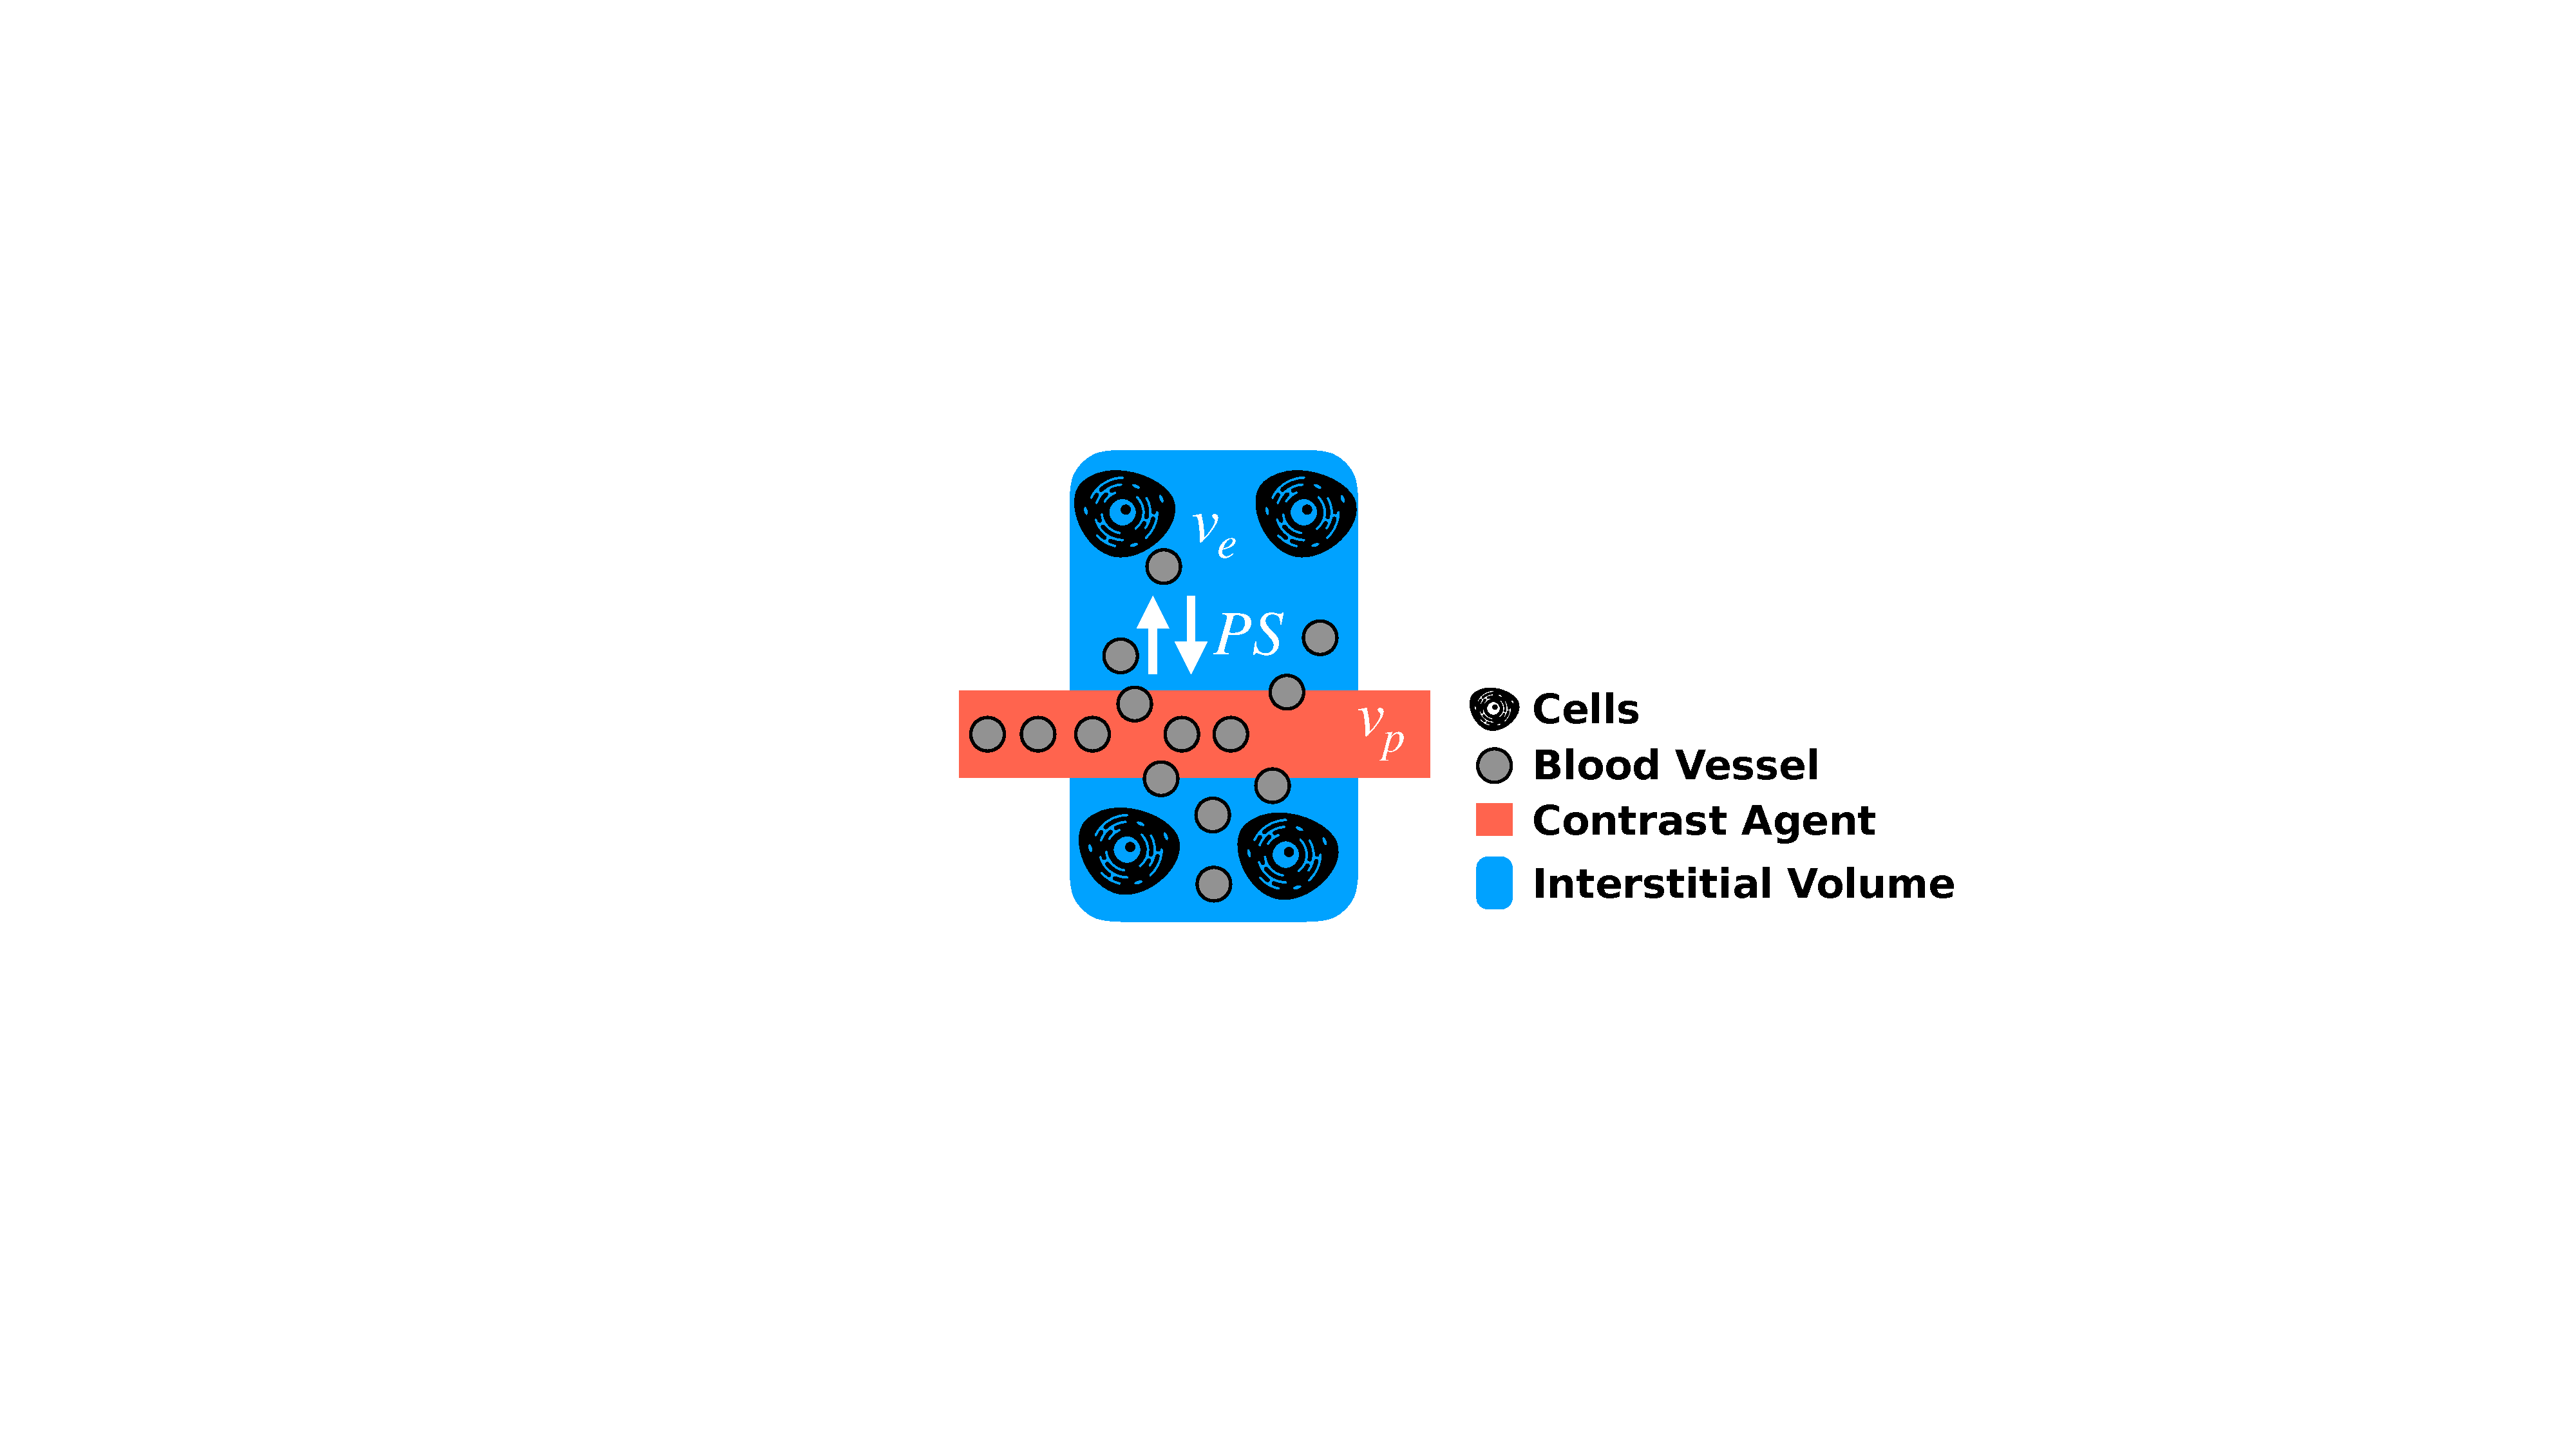
\includegraphics[width=\textwidth]{intro/intro-images/XTofts.pdf}
   \caption[Extended Tofts Model]{Graphical description of the Extended Tofts Model. An arterial input function (\acs{AIF}) governs the introduction of the tracer (grey circles) in the vascular compartment (pink) via a bolus injection. Contrast agent molecules exchanges with the extravascular extracellular space (\acs{$v_e$}, interstitial volume in blue) at a rate given by $PS$, the permeability-surface area product.}
   \label{XTofts}
\end{figure}

Thus, modelling of \acs{DCE-MRI} data to produce quantitative and physiologically relevant values of \acs{K$^{trans}$}, \acs{$v_p$} and \acs{$v_e$} requires an accurate calculation of the \acs{AIF}.
In this thesis, \acs{DCE-MRI} modelling using a traditional small molecule agent (\acs{Gd-DTPA} is used only briefly in Chapter~\ref{ch:HPG} and the \acs{AIF} used in that modelling was measured and published by a former lab member~\cite{Moroz:2013ee}.
Nevertheless, the concepts and introduction to \acs{DCE-MRI} are relevant for several portions of the thesis. 

\section{Thesis structure}

In Chapter~\ref{ch:HPG} we begin by describing a new macromolecular contrast agent and explore its value in describing the tumour microenvironment.
A two-parameter linear model was applied to the contrast agent enhancement curve and we obtained measures of vessel permeability and fractional plasma volume.
These parameters were then used to distinguish between two tumour models.
In Chapter~\ref{ch:HPG2}, we applied this technique to determine whether molecule size played a role in the distribution of a high molecular weight anti-cancer drug (Trastuzumab).
Ultimately we showed that neither vessel permeability nor fractional plasma volume corresponded to presence of bound drug (determined via histological staining), suggesting other barriers that limit distribution of Trastuzumab.
In Chapter~\ref{ch:HPG3} we considered another application of the new contrast agent: can we assess changes in vessel permeability after administering an anti-angiogenic drug?
We discovered that vessel permeability is indeed reduced after drug treatment but along the way we also showed that histologically, hypoxia dramatically decreased after treatment. 
This led us along the journey to develop a new method to assess tumour oxygenation~\emph{in vivo} using MRI and a brief interlude is inserted here to provide some more background information about oxygen and related physiology.
Chapter~\ref{ch:oemri} outlines our technique and describes the use of a blind source separation technique to increase the sensitivity of existing methods. 
We validated the technique in Chapter~\ref{ch:oemri2} with histological staining, and demonstrated utility of a new parameter to separate oxygenation replenishment in different tumour models.
Finally in Chapter~\ref{ch:oemri3} we showcase a typical application of the technique: detection of tumour oxygenation improvements after administering an anti-angiogenic agent. 
We also showed that the tumour implant site has a large bearing on the tumour microenvironment, and no oxygenation improvements are observed if the baseline oxygenation is high.
In Chapter~\ref{ch:futurework} some interesting observations are presented that may be useful starting points for future work in this field.

%    2. Main body
% Generally recommended to put each chapter into a separate file
%% The following is a directive for TeXShop to indicate the main file
%!TEX root = ../diss.tex

\chapter[MRI and histology of vascular function in xenografts using \acs{HPG-GdF}]{Multi-modal magnetic resonance imaging and histology of vascular function in xenografts using macromolecular contrast agent hyperbranched polyglycerol (HPG-GdF)}
\label{ch:HPG}

\section{Introduction}
The vascular network in tumour tissue is abnormal, often resulting in vessels that have variable flow rates and high permeability relative to blood vessels in normal tissue~\cite{McDonald:2002ut}.
Dynamic contrast enhanced magnetic resonance imaging (DCE-MRI) is a useful tool for non-invasively assessing tumour vasculature by imaging and measuring concentrations of \acs{CA} delivered to tumours by the vessels~\cite{OConnor:2012ie,Barrett:2006jx,Leach:2003fy}. \todo[backgroundcolor=blue]{I couldn't search well to confirm this is the first case of the abbrv on this app. Assuming chp 2 is the start - define first}
The appeal of a dynamic, non-invasive approach for measuring tumour vascular function in the clinic is clear.
Such data is applicable in the field of assessing treatment response for vascular targeting therapies~\cite{OConnor:2012ie,Barrett:2006jx,Leach:2003fy}.
In addition to utility as a treatment biomarker, vascular function data may be able to predict which tumours are likely to respond to therapy~\cite{DeBruyne:2012cq,Kelly:2011cf,Bains:2009hh}, or which regions or tumours have greater heterogeneity in their microenvironment~\cite{OConnor:2011jm,Alic:2011hw}.
The issue of limited access for anticancer drugs in solid tumours is significant~\cite{Minchinton:2006gs}, particularly given the efforts to create nanoparticle therapeutics that target the tumour via \acs{EPR} effect~\cite{Jain:2001uf,Iyer:2006gf,Chauhan:2011fi}.
A translatable imaging protocol and suitable contrast agent that yields meaningful, reproducible biomarkers of vascular function could be widely useful in these areas of cancer research.

Low \acs{MW} Gd(III)-based, chelated \acs{CA}s such as Gadovist (MW = 605 Da) exhibit short half-lives and rapid renal clearance~\cite{Weinmann:1984gv}.
With the exception of brain tissue containing a functional blood-brain barrier, low MW Gd agents currently in clinical use diffuse across the vascular endothelium in most normal and neoplastic tissues.
Therefore, a well-established shortcoming of low MW contrast agents is the difficulty of attributing local signal enhancement specifically to either vascular perfusion or vessel permeability.
The ability to characterize physiologically relevant biomarkers of vascular function is desirable for studying the effects of anti-angiogenic treatments in tumours (described in a comprehensive review regarding DCE-MRI and anti-vascular therapies in cancer~\cite{OConnor:2012ie}).
Development and application of macromolecular contrast agents (MCAs) attempt to improve upon DCE-MRI assessment of vascular function by relying on the primarily intravascular nature of \acs{MCA}s.
High MW contrast agents and therapeutics unable to diffuse across the endothelium selectively extravasate from large pores and inter-endothelial cell gaps that characterize the abnormal vessels in the tumour microenvironment~\cite{McDonald:2002ut,Hashizume:2000bq}.
MCAs commonly used in cancer research include albumin, dextran polymers, and PAMAM or PPI dendrimers conjugated with DTPA/DOTA-Gd3+ chelates as described by Tang et al.~\cite{Tang:2013fi}.
The size of \acs{MCA}s in use or under development ranges considerably, but may be as small as a 90 kDa albumin conjugate, or one of a range of dextran sizes~\cite{Barrett:2006jx}.
Particles less than 5 nm in size have been found to leak rapidly from tumour vasculature, whereas those in the 5-8nm range are limited to leaking from hyperpermeable vessels; those greater than 8nm are thought to have minimal leakage~\cite{Kobayashi:2004vq,Sato:2001tt}.
The most commonly used \acs{MCA}s in preclinical research are albumin based; however, these are not translatable to the clinic due to immunogenicity concerns~\cite{Ogan:1987tg}.
Signal enhancement is linked to contrast agent concentration within the tumour blood vessels at early time points after injection for \acs{MCA}s that remain intravascular, such that tumour plasma volumes (Vp) can be determined.
Rates of \acs{MCA} leakage from hyperpermeable vessels may then be modeled to evaluate permeability, since extravascular accumulation of the agents will manifest as increased enhancement in repeat images~\cite{Ogan:1987tg,Turetschek:2004bw}.
This analysis is dependent on the assumption that the \acs{MCA}s have unidirectional flow and do not leak back into the plasma, and that the concentration in the plasma is constant, creating a permeabilitylimited environment.
In this study we investigated a multi-modal, high MW contrast agent, \acs{HPG-GdF}: hyperbranched polyglycerol (HPG) molecules doubly labeled with Gd-DOTA and a fluorescent marker.
HPGs are soluble, globular, asymmetrical, have low immunogenicity and are highly biocompatible molecules with low polydispersity~\cite{Saatchi:2012hc,Kainthan:2006ce,Saatchi:2012gc}.
HPG has been previously tested as a human serum substitute~\cite{Kainthan:2008ek} and as a drug delivery vehicle due to its versatility as a chemical, such that drugs, Gd chelates, fluorescent and radiolabels may all be attached to it~\cite{Shenoi:2013id}.
Many other \acs{MCA}s, including Gd-albumin, are highly viscous, which can limit the applicable dose~\cite{Imranulhaq:2012ij}.
The MW of \acs{HPG-GdF} is tunable to required applications, and a biodegradable version of HPG is also available for potential use~\cite{Shenoi:2013id}.
The \acs{HPG-GdF} described in this study is 583kDa and 8-10nm in diameter; synthesis of \acs{HPG-GdF} has previously been described~\cite{Saatchi:2012hc}.
A significant advantage of \acs{HPG-GdF} is that it is a multi-modal agent, with both fluorescent and Gd-chelate labels that permit histological validation of observations made using MRI, including determining the degree to which the agent extravasates from the vasculature.
Previous studies have also used 111In as a SPECT label with utility for biodistribution studies~\cite{Saatchi:2012hc}.
In this work, we employed comprehensive histological methods to investigate the microregional location of \acs{HPG-GdF} in two human colorectal xenograft models, and used this information to interrogate observations made non-invasively using DCE-MR imaging of the same agent in the same tumours.

\section{Methods}

\subsection{Mice and tumours}

Female NOD/SCID mice were bred and housed in institutional animal facilities; experiments in this study were approved by the Animal Care Committee of the University of British Columbia.
Fiducial markers were constructed of PE-50 polyethylene tubing (inner diameter, 0.58mm) and filled with paraffin wax and saline, creating an MR-visible interface~\cite{Bains:2009hh}.
Marker tubes were implanted subcutaneously in the sacral region of mice, in a craniocaudal orientation, 2 days prior to subcutaneous implantation of tumours.
Both histological and MR modalities imaged slices in the plane perpendicular to the marker tube to minimize angular differences between serial MR image slices obtained over multiple sessions, and for corresponding cryosections in histological processing.
HCT116 or HT29 human colorectal carcinoma cells obtained from the American Type Culture Collection (ATCC) were implanted near the fiducial tubes such that the tumours grew around the tubes.
Tumours were used when diameters reached 8-12 mm.
Mice were anaesthetized with isoflurane for the duration of imaging sessions.
Animals were positioned supine on the custom surface coil apparatus fitted with a lid lined by a temperature-controlled, water-filled heating blanket.
Body temperature and respiration rate were monitored throughout imaging.
Following their final scan animals were administered a 35 $\mu$L intravenous dose of 0.6 mg/mL carbocyanine (DioC7(3); Molecular Probes, Eugene, OR, USA) in 75\% dimethylsulfoxide as a fluorescent dye indicator of vessel perfusion in histological measures, and euthanized 5min after injection.
Some animals received \acs{HPG-GdF} and tumours were collected at early time points for histological analysis only, with no MR-imaging.
Tumors were embedded and frozen vertically in optimum cutting temperature medium (OCT; Tissue-TEK) using their fiducial markers for guidance.

\subsection{Contrast agents and dosage}

Hyperbranched polyglycerol (HPG-GdF) (Fig.~\ref{hpgpaper1:fig1}): 583 kDa HPG was synthesized at the University of British Columbia (D. Brook’s laboratory, Department of Chemistry) with a narrow polydispersity of PDI = 1.01 by ring-opening multibranching polymerization of glycidol using dioxane as the reaction medium, according to a published procedure~\cite{Kainthan:2006ce}.
HPG was derivatized with p-NH2-benzyl-DOTA (Macrocyclics, Dallas, TX, USA) at 20$\mu$g Gd per mg HPG and tagged with Alexa Fluor 647 (Invitrogen Life Technologies, Burlington, ON, Canada) as previously described (20).
The biological half-life of HPG-Gd (with no fluorescent tag) in mice has previously been examined in biodistribution studies and was reported as 32.6 h (20).
HPG-GdF was administered as a 6 $\mu$L/g bolus dose from 100 mg/mL (0.2 mM) using an intravenous (i.v.) catheter; therefore, the administered molar dose of HPG was 1.2 nmol/g and that of the chelated Gd(III) was 240-360 nmol/g (determined according to an estimated 200-300 chelates per HPG molecule (20)).
Assuming a blood volume of 5\% of mouse body weight, peak blood concentration of \acs{HPG-GdF} is 24$\mu$M.
This value has been used to normalize relative tissue concentrations (Fig.~\ref{hpgpaper1:fig2}(B)) and to calculate the fractional plasma volume (fPV; see Section 2.4).
The relaxivity of \acs{HPG-GdF} has previously been measured and reported to be 1075 mM$^{-1}$s$^{-1}$1, which is approximately 300 times greater than that of Gadovist (3.58 mM$^{-1}$1 s$^{-1}$1) (20).
Gadovist (Bayer Healthcare, Toronto, ON, Canada; 607.4 Da) was administered by i.v. catheter as a 5 $\mu$L/g bolus dose from 60 mM solution, for an administered molar dose of Gadovist of 300 nmol/g.
All in-scanner i.v. injections were performed using a power injector at a rate of 1 mL/min.
An extended fluid line connected to the i.v. catheter secured to the tail vein of the mice permitted remote initiation of injections outside the scanner room.
Injections included a small volume (<40 $\mu$L) of heparinized saline followed by the contrast agent, which was then followed by a 20 $\mu$L flush of heparinized saline.

\begin{figure}[htbp]
 \begin{center}
 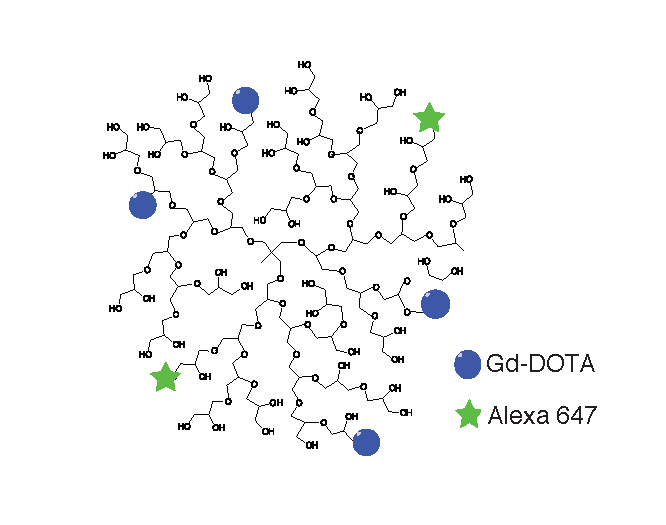
\includegraphics[width=\textwidth]{hpg/hpg-paper1-images/hpg_fig1-hpgdf.pdf}
 \caption{HPG-GdF. The 583 kDa globular Hyperbranched PolyGlycerol (HPG) molecules are derivatized with p-NH$_2$-benzyl-DOTA (Macrocyclics) at 20 $\mu$g Gd per mg HPG (approximately 300 chelates per molecule) and tagged with Alexa Fluor 647 dye, as previously described (\cite{Saatchi:2012hc}.}
 \label{hpgpaper1:fig1}
 \end{center}
\end{figure}

\subsection{MRI acquisition}

All MRI experiments were performed at the UBC MRI Research Centre on a 7T Bruker BioSpec 70/30 scanner at room temperature with a combination of volume (transmit)/surface (receive) coil.
Each imaging session began with axial RARE T$_2$-weighted images for morphological reference and precise alignment of imaging plane.
Further T$_1$-weighted RARE images were acquired for qualitative assessment of contrast agent distribution.
During the first scanning session, T$_1$ and flip angle maps were acquired prior to a DCE-MRI experiment, followed by another T$_1$ measurement.
At each imaging session slice location and orientation were adjusted to match previous sessions.
T$_1$ measurements and flip angle mapping were performed using a multi-slice FLASH variable flip angle experiment (FLASH TR/TE = 500/2.75, FA = 10$^{\circ}$, 20$^{\circ}$, 30$^{\circ}$, 40$^{\circ}$, 50$^{\circ}$, 60$^{\circ}$, 70$^{\circ}$, 80$^{\circ}$, 90$^{\circ}$, 100$^{\circ}$, 110$^{\circ}$, 120$^{\circ}$, 130$^{\circ}$, 140$^{\circ}$, 150$^{\circ}$, 160$^{\circ}$, 170$^{\circ}$, 180$^{\circ}$, 190$^{\circ}$, 200$^{\circ}$, 215$^{\circ}$) and data were fit simultaneously for T$_1$ and the B1 scaling factor map.
DCE-MRI data was collected at 2.24 s time resolution (FLASH; TR/TE = 35/2.75; FA = 40; NR = 1200).
T$_1$ and DCE-MRI experiments all had identical geometry (matrix = 128 x 64; three slices; voxel size = 0.33 mm x 0.297 mm x 1.5 mm; 2.5 mm slice separation).
A follow-up T$_1$ measurement was performed (FLASH; TR/TE = 35/2.75; FA = 10$^{\circ}$, 20$^{\circ}$, 30$^{\circ}$, 40$^{\circ}$, 50$^{\circ}$, 60$^{\circ}$, 80$^{\circ}$, 100$^{\circ}$, 120$^{\circ}$) and the B$_1$ scaling factor map from the baseline acquisition was used to determine post-contrast T$_1$ (assuming that B$_1$ scaling does not change due to contrast injection).
Difference maps of relaxation rates $\delta$R$_1$ = 1/T$_1$(post-contrast) - 1/T$_1$(precontrast) were constructed for a measure of contrast agent concentration.
Animals received two DCE-MRI scans 24-48h apart, with Gadovist administered and scanned at the first session and \acs{HPG-GdF} administered and scanned at the subsequent session with tumours collected for histological processing at about 60 min post administration of their \acs{HPG-GdF}.

\begin{figure}[htbp]
 \begin{center}
 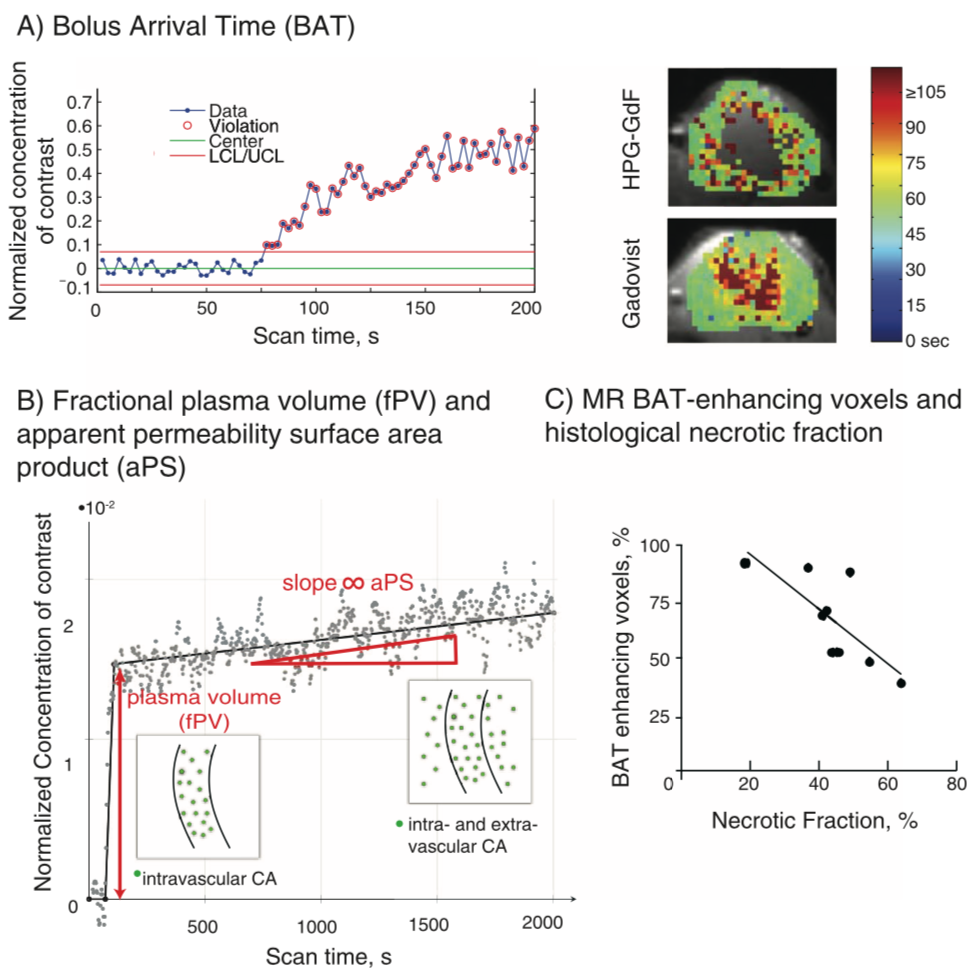
\includegraphics[width=\textwidth]{hpg/hpg-paper1-images/hpg_fig2-bat.png}
 \caption{MR-derived parameters to measure vascular function using \acs{HPG-GdF}: bolus arrival time (BAT), fractional plasma volume (fPV) and apparent permeability-surface area product (aPS). (A) Sample curve showing change in concentration of \acs{CA} as a function of scan time. The first violation (circle) is identified by Rule (1) at Frame 31, corresponding to a BAT of t = 77.5 s. The centre (mean) and upper (UCL) and lower (LCL) control limits ($\pm$3 SDs) are drawn for reference. Sample BAT parameter maps from \acs{HPG-GdF} and Gadovist obtained from the same HT29 xenograft imaged 24h apart show that \acs{HPG-GdF} is slower to arrive; both \acs{CA}s arrive most quickly at the tumour margins. (B) \acs{HPG-GdF} enhancement curve shown for a full imaging period where the bolus arrival is seen as a significant jump in enhancement from which the \acs{fPV} is derived as the concentration at the start relative to the plasma concentration, since the \acs{CA} is largely intravascular at that early time. The \acs{aPS} is the slope of the enhancement after the bolus arrival. The concentration curves are shown as ratio of tissue concentration to blood peak concentration (24 $\mu$M) (C) The fraction of MR-measured \acs{HPG-GdF} BAT-enhancing voxels has a negative association with the proportion of necrotic tissue determined in histological sections.}
 \label{hpgpaper1:fig2}
 \end{center}
\end{figure}

\subsection{MRI data analysis}

Regions of interest (ROIs) were drawn on T2-weighted RARE images to outline the tumour using ImageJ (NIH), and all other MR analysis was performed using MATLAB (MathWorks, R2009a) and Python.
T$_1$ and flip-angle maps were calculated from variable flip-angle data with a slice-profile correction based on simulations described by Parker et al.~\cite{Parker:2001wj}.
The same method was extended to provide time-dependent T$_1$ and concentration-time in DCE data series.
Areas under the curves (AUCs) were numerically integrated starting from the bolus arrival time, or, for tumour-averaged AUC, starting from the common injection time point and extended to the indicated time points (1 and 37 min).
Bolus arrival time (BAT) is the time when detectable signal enhancement begins for a voxel (Fig.~\ref{hpgpaper1:fig2}(A)) due to contrast agent arrival.
Based on the control-chart decision criterion and the Western Electric decision rules from MATLAB’s statistical toolbox~\cite{Shewhart:1931tq}, voxel enhancement was detected as a positive change from baseline signal for three consecutive timepoints (frames) (i) in the same direction, (ii) starting 5 s before the time of injection or later and (iii) for at least 10\% of all timepoints following initial change of signal away from baseline.
Therefore, voxels with a finite BAT and for which at least 10\% of the following intensities were classified as enhancing by the BAT criteria were called enhancing voxels, whereas all other voxels were labeled as non-enhancing.

A change from baseline was determined to have occurred
when any one of the following inclusion criteria were met:

\begin{enumerate}
	\item any point fell outside of 3 SDs from the average baseline concentration, or
	\item two of three consecutive points fell outside of the 2 SD limit on the same side of the mean, or
	\item four of five consecutive points fell outside of the 1 SD line, on the same side of the centre line, or
	\item eight consecutive points all fell on one side of the centre line.
\end{enumerate}

In the illustrated example (Fig.~\ref{hpgpaper1:fig2}(A)), a change from the mean was identified at Frame 31 and the two following scans by Rule (1); therefore, the BAT point was selected as Frame 30.
The centre line (mean of baseline) and upper and lower control limits ($\pm$3 SDs) are drawn for reference.

\subsubsection{Pharmacokinetic modeling of DCE-MRI data}

\textit{Gadovist.} The extended Tofts model was used and three parameters resulted: K${trans}$, vE, and vP~\cite{Sourbron:2011ce}.
The arterial input function (AIF) for this model was determined previously by our laboratory using a projection-based method~\cite{Moroz:2013ee}.
\textit{HPG-GdF.} A two-parameter linear model was applied~\cite{Pathak:2005gu}.
Two parameters were used to characterize the \acs{MCA} time curves: (1) the rapid increase at the time of injection (related to the \acs{fPV}) and (2) the slope of the later enhancement (aPS) (Fig.~\ref{hpgpaper1:fig2}(B)).
The relative plasma volume could be determined from the ratio of concentrations in the voxel of interest to the concentration in whole blood in the seconds after injection, since extra-vascular spread of the agent was negligible at this time.
The slope of the concentration time curve following contrast arrival is proportional to the permeability-surface area product (PS) when the assumption of a permeability-limited environment is valid.
However, in the highly variable tumour microenvironment, extravasation of contrast agent may deplete the intra-vascular concentration appreciably in conditions of high permeability, which would increase the relative contribution of perfusion to the composite measure of PS.
To stress that the interpretation of this slope value depends on the assumption of a permeability-limited environment, we term the slope the apparent permeability-surface area product (aPS)~\cite{DaldrupLink:2004gy,Dafni:2002kb}.

\subsection{Histology}

Cryosections of 10 $\mu$m were obtained along the plane perpendicular to the fiducial marker at depths corresponding to MR imaged slices.
Sections were imaged for DiOC7(3) and HPGGdF native fluorescence and fixed in acetone-methanol for 10min prior to staining and re-imaging for CD31 (PECAM/ CD31) and Hoechst 3342, labeling vascular endothelium and cell nuclei, respectively.
Sections were imaged as previously described~\cite{Kyle:2007ch} using a system of tiling adjacent microscope fields of view such that images of entire tumour cryosections were captured at a resolution of 1.5 $\mu$m/pixel.
Using both fiducial and anatomical landmarks, histological sections were chosen to match the MR slices.
Using ImageJ~\cite{Collins:2007jr} and user-supplied algorithms, digital images were superimposed and manually cropped to tumour tissue boundaries; staining artifacts and necrosis were also removed for some analyses.
Positive fluorescence for CD31 and DiOC7(3) images was obtained by applying a threshold, with neighboring positive pixels grouped as ``objects''.
The average distance of tissue to the nearest vascular object was reported as a repeatable measure of vascular density.
Perfused vessel fraction (PF) was calculated as the proportion of CD31-positive objects that had at least 20\% overlap with positive DiOC7(3) or \acs{HPG-GdF} pixels on the overlaid image.
Data for individual tumours were displayed as mean $\pm$ SEM values.
HPG-GdF extravasation was assessed by its distance from blood vessels: pixels from the \acs{HPG-GdF} fluorescence image were sorted according to their distance from vascular objects and the average \acs{HPG-GdF} fluorescence intensity was reported.

\begin{figure}[htbp]
 \begin{center}
 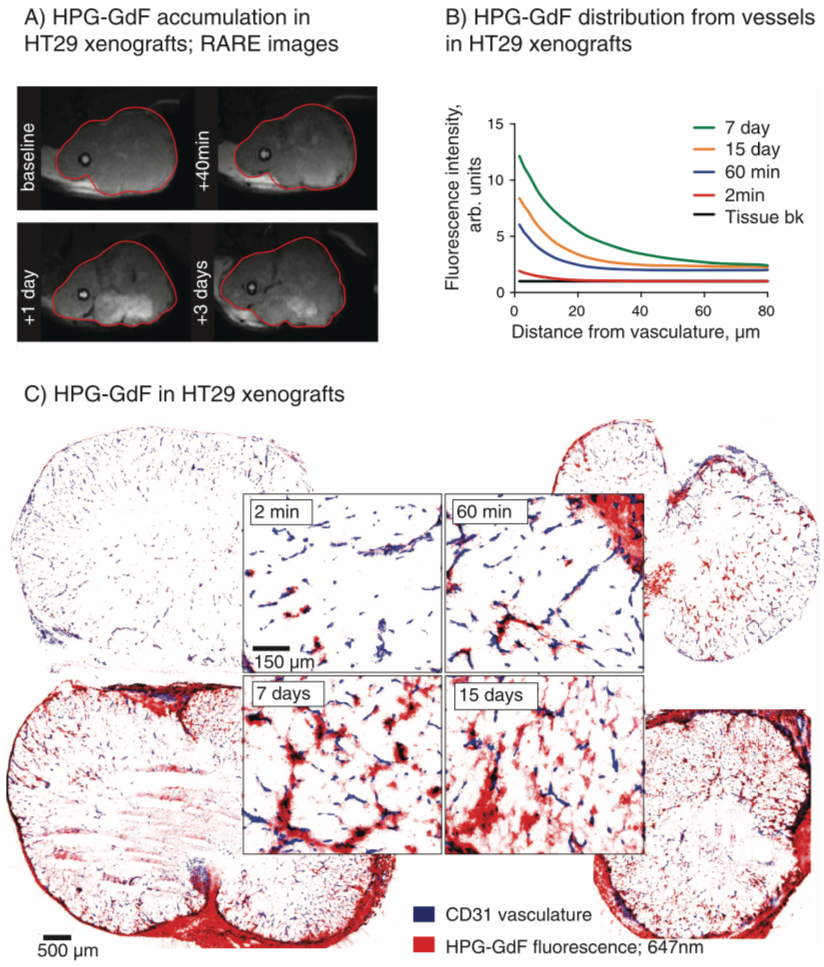
\includegraphics[width=\textwidth]{hpg/hpg-paper1-images/hpg_fig3-hpgdistribution.png}
 \caption{Accumulation and distribution of \acs{HPG-GdF} in HT29 xenografts. (A) T$_1$-weighted MR-RARE images show signal enhancement at 40 min that increases with longer exposures (HT29 tumours outlined in red). (B) Quantitative analysis of \acs{HPG-GdF} distribution relative to CD31-positive vessels shows extravasation of \acs{HPG-GdF} and distribution away from vessels to a limited distance, with a maximum at 7 days. (C) Whole tumour maps of \acs{HPG-GdF} (red) in relation to vasculature (blue) show that at early (2 min) timepoints \acs{HPG-GdF} is primarily overlapped with vasculature, but by 60 min there is substantial heterogeneity, where some vessels have greater amounts of perivascular \acs{HPG-GdF} than others. \acs{HPG-GdF} accumulates over several days but does so heterogeneously, and does not distribute through tumour tissue even after prolonged exposures.}
 \label{hpgpaper1:fig3}
 \end{center}
\end{figure}

\section{Results}

\subsection{HPG-GdF accumulates in tumour tissue in the extravascular space but does not distribute far from vasculature}

Averaged data from whole HT29 tumour xenograft images obtained using MRI and histology showed accumulation of \acs{HPG-GdF} over time (Fig.~\ref{hpgpaper1:fig3}(A)), as previously described~\cite{Saatchi:2012hc}.
HPG-GdF fluorescence was detectable within or very near to CD31-labeled tumour vessels as early as 2 min following contrast agent injection (Fig.~\ref{hpgpaper1:fig3}(B), (C)).
More HPGGdF fluorescence accumulated in histological tumour sections over time, but very little agent was observed at distances farther than 40 $\mu$m from the vasculature, even at 7 and 15 days (Fig.~\ref{hpgpaper1:fig3}(B), (C)).
By 60min there was extravascular accumulation of \acs{HPG-GdF} around some vessels, but considerable inter-vessel heterogeneity was observed.
Some vessels showed no \acs{HPG-GdF} fluorescence (Fig.~\ref{hpgpaper1:fig3}(C)).

\subsection{Bolus arrival time (BAT) for \acs{HPG-GdF} as a screen for viable tissue}

Maps of BAT overlaid on T$_1$-RARE images for both Gadovist and \acs{HPG-GdF} are shown in Fig.~\ref{hpgpaper1:fig4}, Rows 1 and 2.
A pattern of faster contrast enhancement at the tumour margins was consistent for both contrast agents.
While Gadovist eventually distributes to all the tissue, many voxels fail to enhance with \acs{HPG-GdF} within the 37 min imaging period.
Comparison of \acs{HPG-GdF} BAT-enhancing voxels with a histological image delineating viable versus necrotic tissue (Fig.~\ref{hpgpaper1:fig4}, Rows 2 and 3) shows that the non-enhancing voxels consistently corresponded to large areas of tumour necrosis.
A negative association was seen between the necrosis fraction determined by histology and the fraction of enhancing voxels for \acs{HPG-GdF} (Fig.~\ref{hpgpaper1:fig2}(C)).
For subsequent analysis of vascular function, only voxels enhancing with \acs{HPG-GdF} using the BAT criteria were evaluated.

\begin{figure}[htbp]
 \begin{center}
 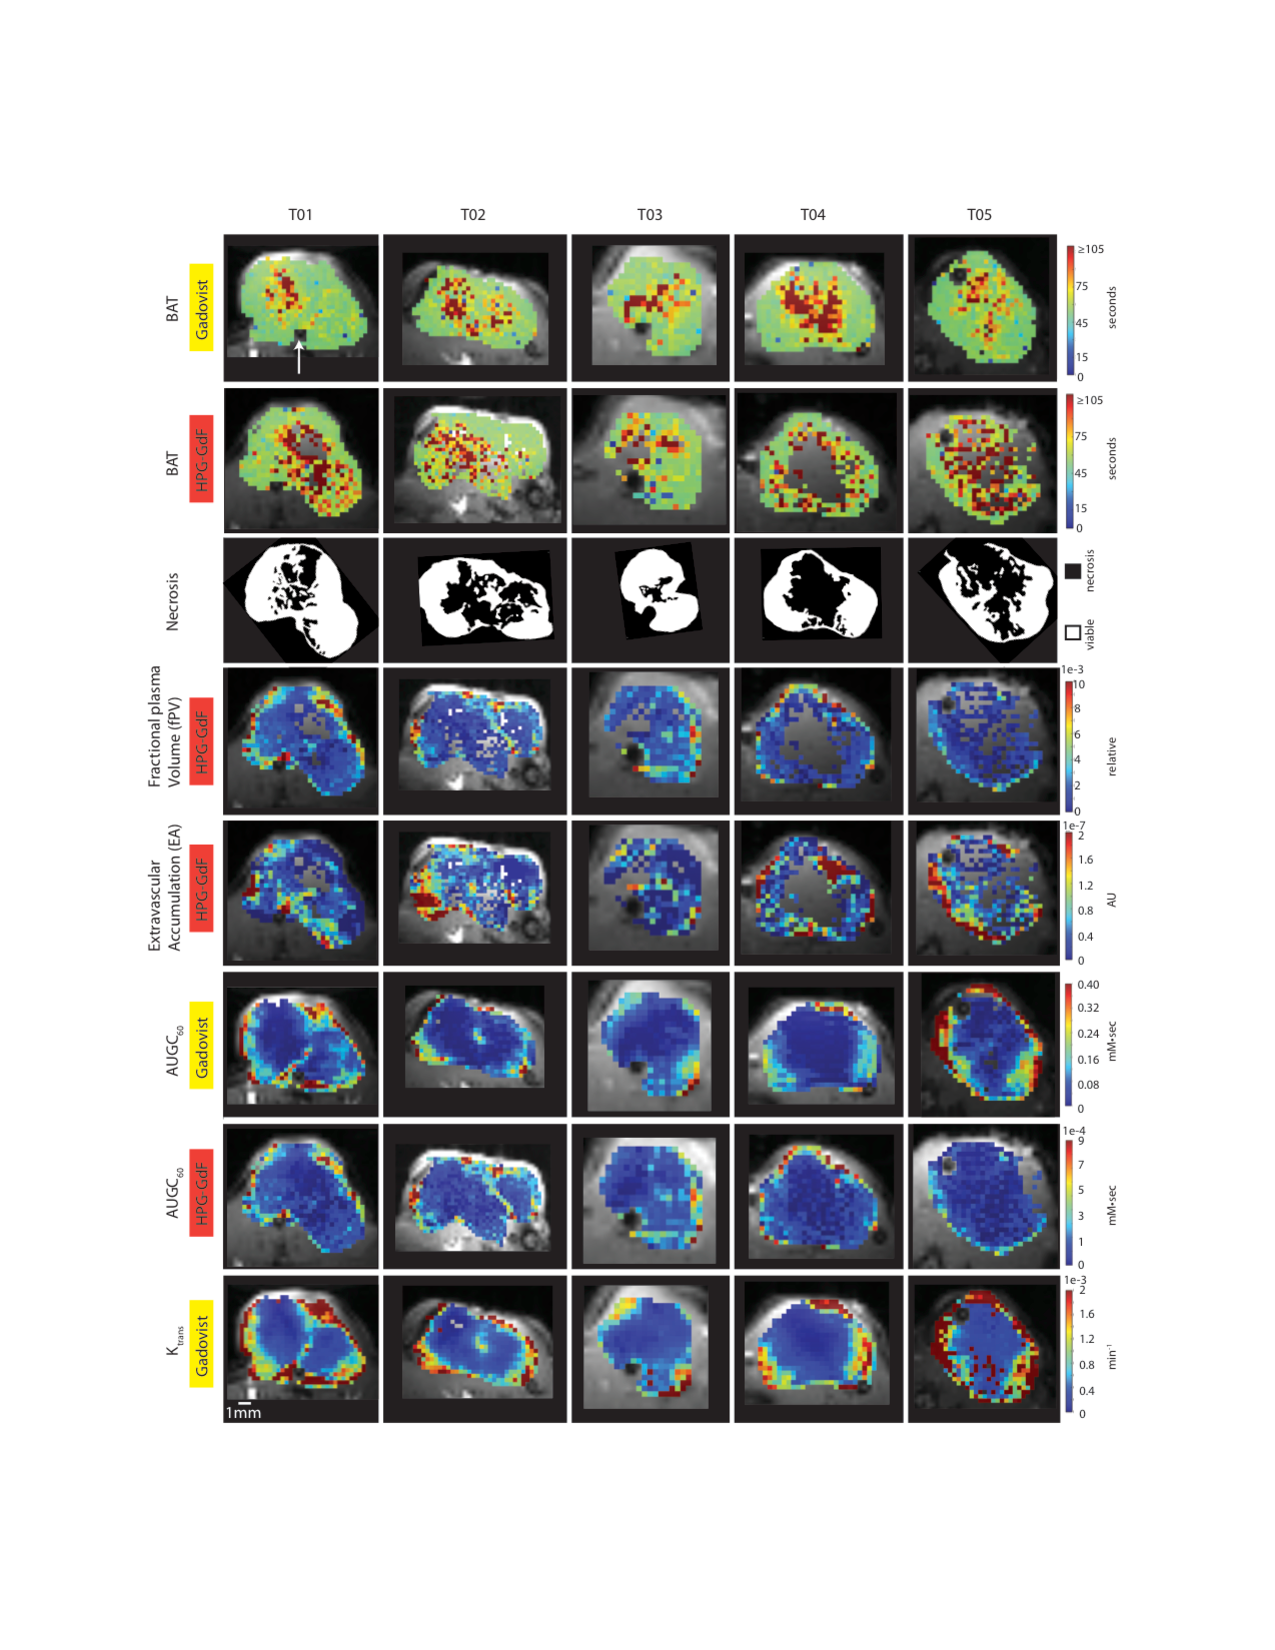
\includegraphics[width=0.8\textwidth]{hpg/hpg-paper1-images/hpg_fig4-ht29.pdf}
 \caption{Vascular function in HT29 xenografts. Whole-slice maps are presented for individual HT29 tumours (T01-T05, vertical columns) for parameters derived from MR imaging of Gadovist (BAT, AUGC60, K$^{trans}$), MR imaging of \acs{HPG-GdF} (BAT, fPv, \acs{aPS}, AUGC60) and histological imaging (necrosis). Good slice matching between imaging sessions is achieved using implanted fiducial marker tubes, an example of which is shown for tumour T01, Row 1, where the arrow points to the dark region where the tube is resting between the tumour and the back of the animal.}
 \label{hpgpaper1:fig4}
 \end{center}
\end{figure}

\subsection{Fractional plasma volume (fPV) and apparent permeability-surface area product (aPS) as measures of vascular function}

HPG-GdF-enhancing voxels were further characterized for their plasma volume (fPV) by calculating the magnitude of the rapid signal increase after injection and for their extravascular accumulation (apparent permeability-surface area product, \acs{aPS}) by measuring the slope of the enhancement curve after the initial increase for the duration of the DCE scan (0-2000 s).
The patterns of high and low \acs{fPV} and \acs{aPS} were often similar to each other, though there are notable differences.
A linear regression analysis comparing \acs{fPV} with \acs{aPS} for whole-slice averages yields an R$^2$ of 0.11, suggesting they are independent of each other.
As a detailed example, tumour HT01 has a region of high \acs{aPS} and low \acs{fPV} (Fig.~\ref{hpgpaper1:fig5}(A)), as well as a region exhibiting the opposite, with high \acs{fPV} and low \acs{aPS} (Fig.~\ref{hpgpaper1:fig5}(B)).
The corresponding histological section seemed to validate these observations, where the region with high \acs{fPV} has a greater density of CD31-stained vessels and the region with greater \acs{aPS} has more \acs{HPG-GdF} in the extravascular compartment.
While histological data enables a detailed view of \acs{HPG-GdF} accumulation, the actual rate of extravasation may only be determined by the dynamic MR data, as illustrated by the schematic enhancement curve (Fig.~\ref{hpgpaper1:fig5}(C)).
The corresponding K${trans}$ map derived from Gadovist concentrations shows high values in both the high \acs{aPS} and high \acs{fPV} regions of this tumour (Fig.~\ref{hpgpaper1:fig4}, Column 1).
Therefore, both \acs{fPV} and \acs{aPS} played important roles contributing to overall tumour vascular function, had measurable intra-tumour heterogeneity and produced data that was distinct from and more informative than DCE-MRI derived parameters for Gadovist.

\begin{figure}[htbp]
 \begin{center}
 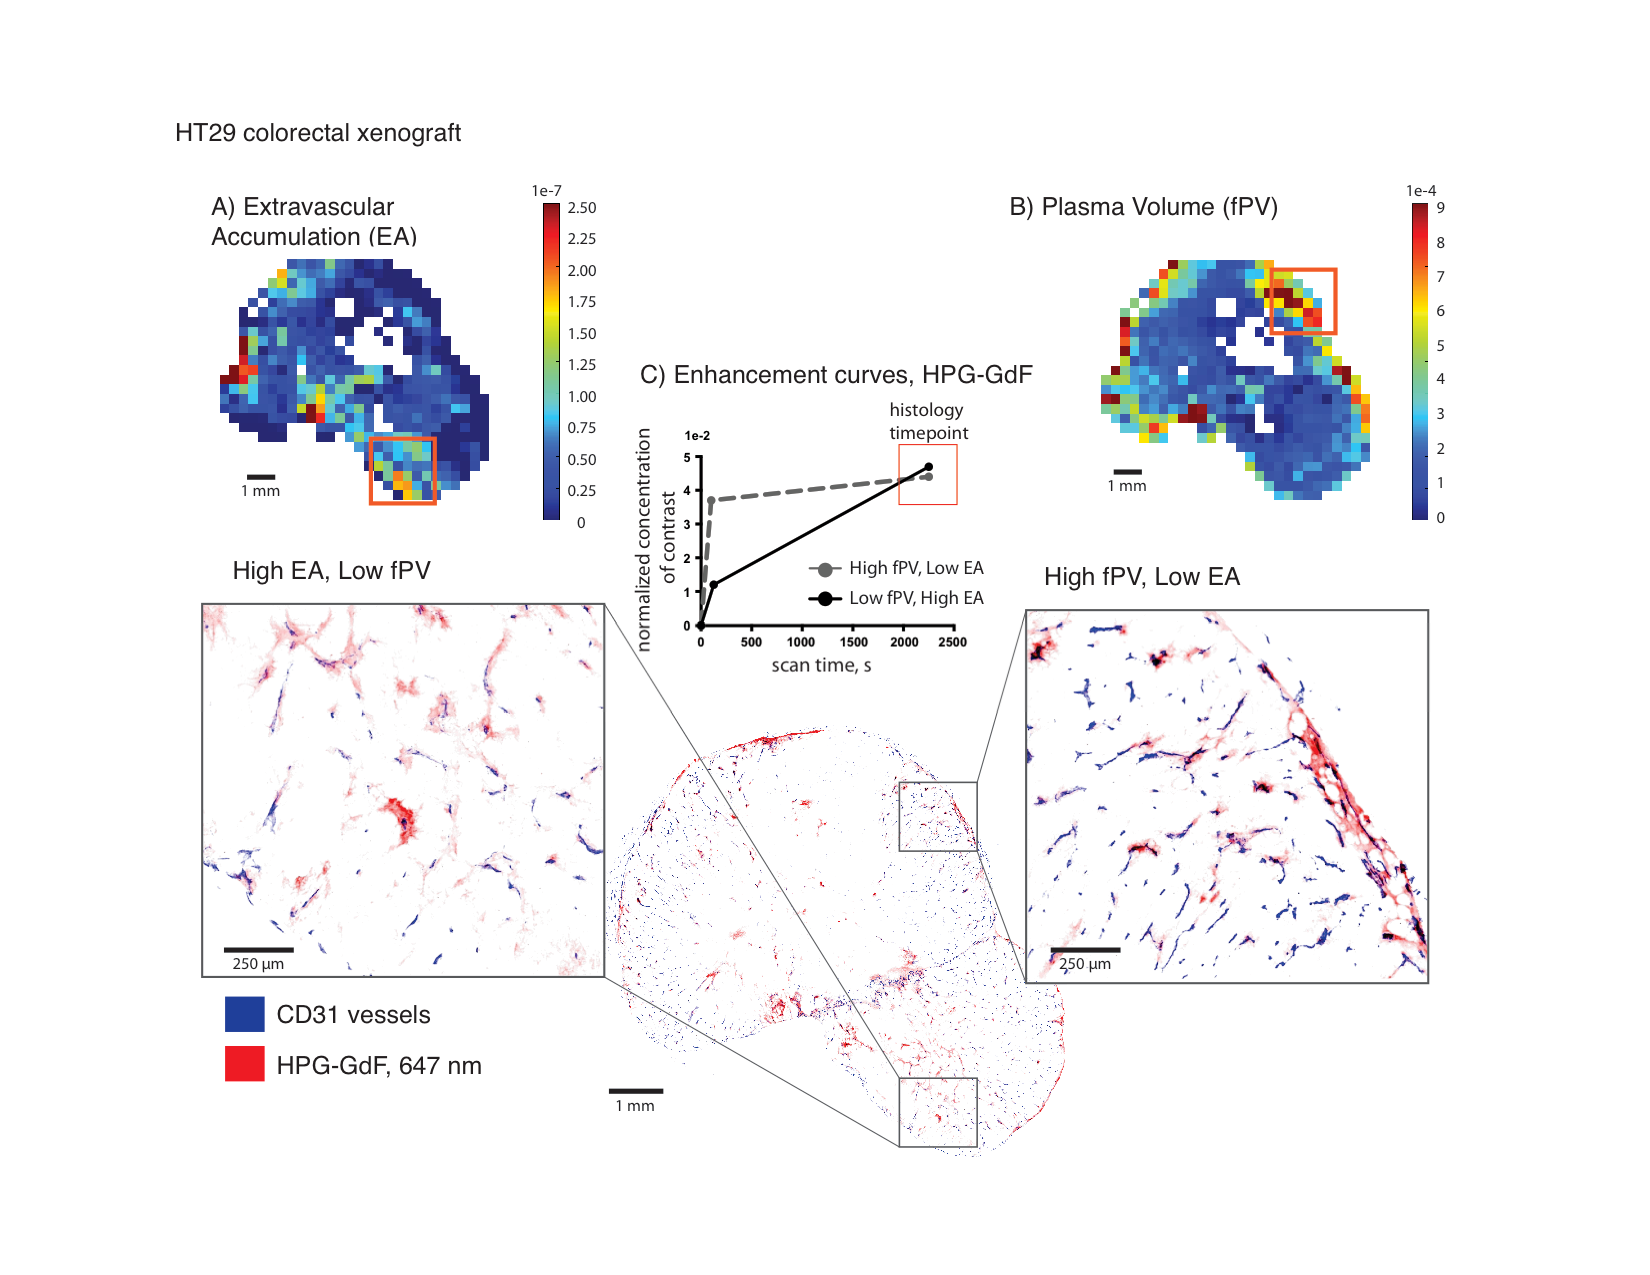
\includegraphics[width=\textwidth]{hpg/hpg-paper1-images/hpg_fig5-ht29fpv.pdf}
 \caption{fPv and \acs{aPS} in HT29 xenograft.
 Whole-slice parameter maps are presented for HT29 tumour (T01) with the corresponding histological image depicting CD31 stained vessels (blue) and \acs{HPG-GdF} native fluorescence (red).
 A region with high \acs{aPS} values that does not correspond to high \acs{fPV} is magnified (A) and compared with a region having high \acs{fPV} that does not correspond to high \acs{aPS} (B).
 The high \acs{fPV} region has notably greater vascular density, and \acs{HPG-GdF} is clearly seen overlapping with vessels (black) or accumulating in the extravascular space.
 The high \acs{aPS} region also has \acs{HPG-GdF} in the extravascular space.
 The dynamic MR-derived parameters are better able to illustrate the functional features of tumour vasculature than are the static histological data, which only reflects the environment at a single, terminal endpoint (C).}
 \label{hpgpaper1:fig5}
 \end{center}
\end{figure}

\begin{figure}[htbp]
 \begin{center}
 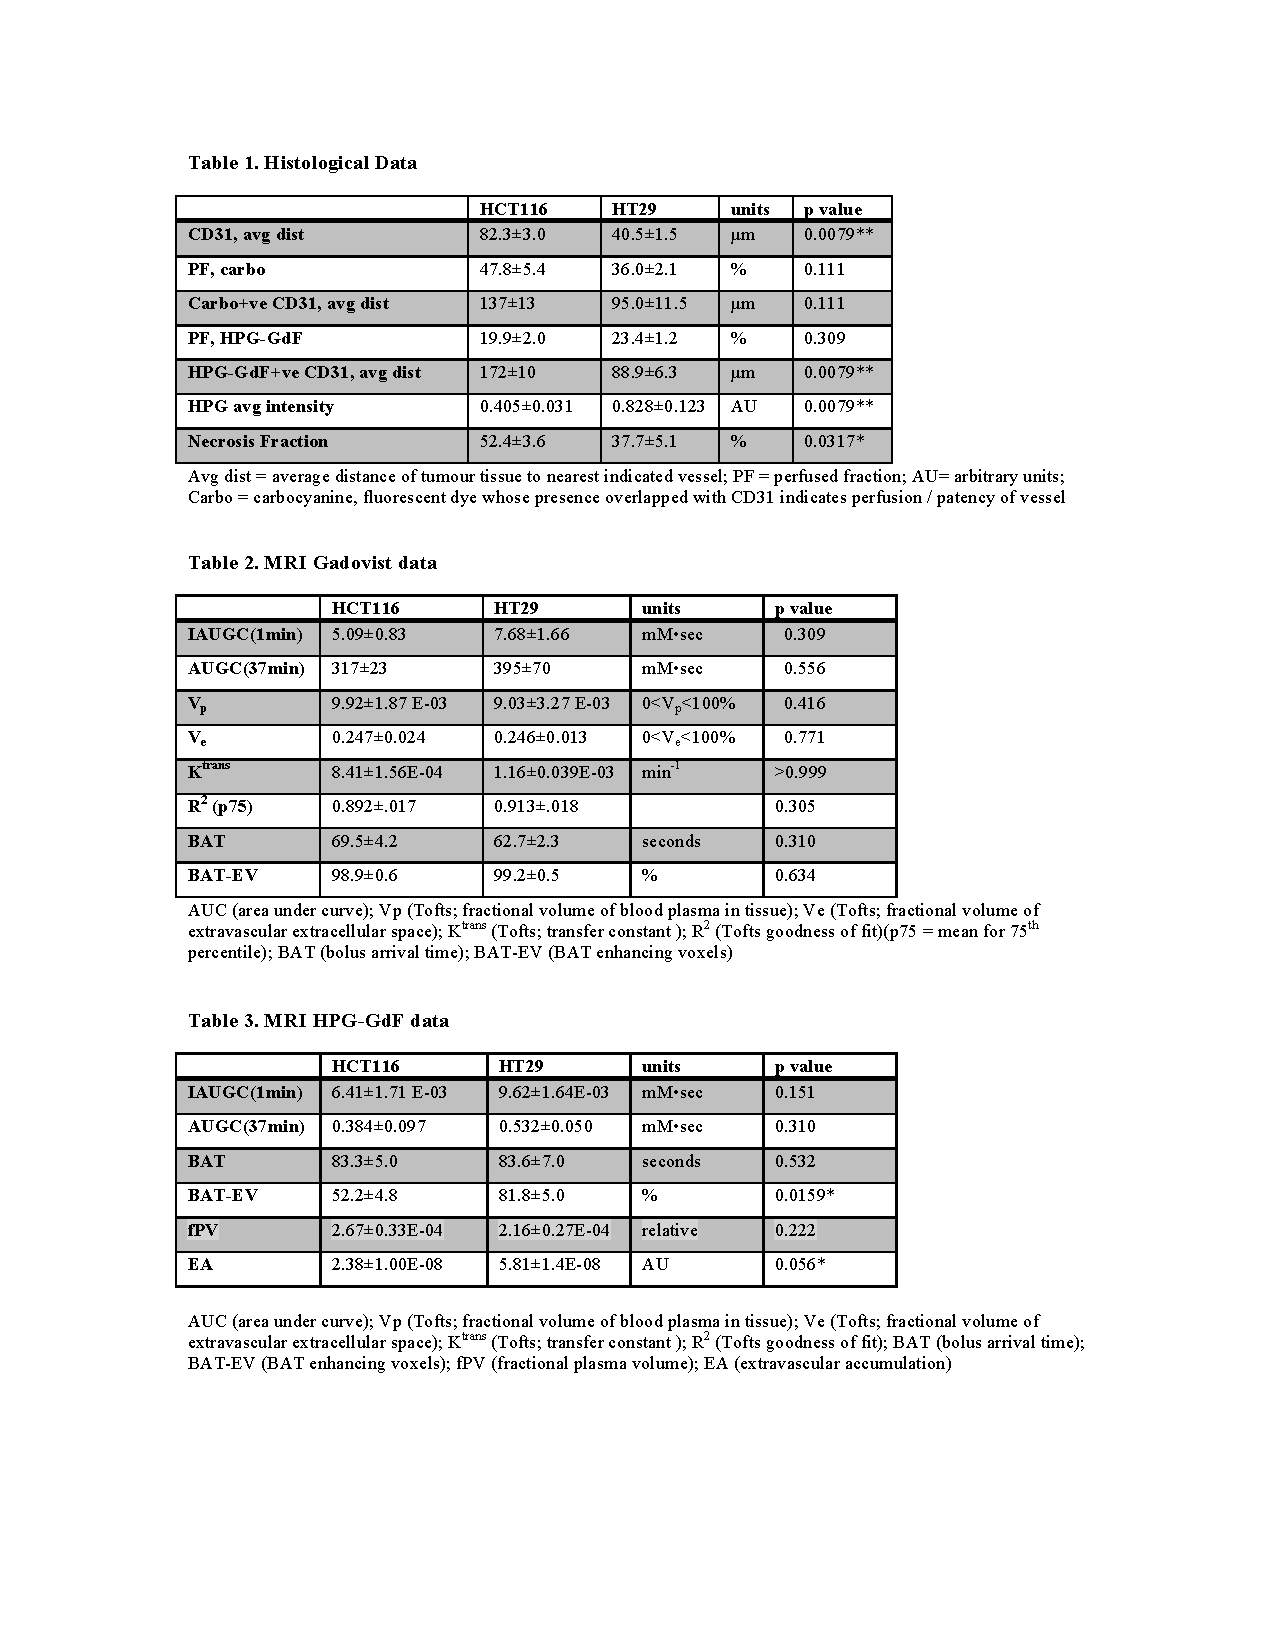
\includegraphics[width=\textwidth]{hpg/hpg-paper1-images/hpg_tables.pdf}
 \caption{ }
 \label{hpgpaper1:tables}
 \end{center}
\end{figure}

\subsection{Variable vascular function in HCT116 and HT29 human colorectal xenografts}

HPG-GdF accumulated to a greater degree in HT29 colorectal xenografts relative to HCT116, and this was seen at all distances from vessels (Fig.~\ref{hpgpaper1:fig6}(A)).
HCT116 and HT29 colorectal xenografts grow at similar rates in mouse models but exhibit distinct vascular function parameters (data summarized in Table 1).
Overall, HT29 tumours possessed a greater density of vessels (CD31 average distance was 82.3 $\pm$ 3.0 $\mu$m for HCT116 and 40.5 $\pm$ 1.5 $\mu$m for HT29, p < 0.05*).
However many vessels were unlabeled for the fluorescent dye (carbocyanine) used as a histological perfusion marker; the density of perfused vessels was similar between the two xenograft models (CD31 vessels labeled for carbocyanine, PF, was 47.8$\pm$5.4\% for HCT116 and 36.0$\pm$2.1\% for HT29, p > 0.05).
The density of vessels labeled for HPG-GdF fluorescence was much greater in HT29 tumours (HPG-GdF+ve CD31, average distance was 172$\pm$10$\mu$m for HCT116 and 88.9 $\pm$6.3$\mu$m; p<0.05*).
In addition to a greater density of HPGGdF-positive vessels, the high MW contrast agent was able to accumulate to a greater degree in the extravascular space around vessels in HT29 cells.
This effect can be seen in the histological images of the compared tumour models collected 60min post HPG-GdF administration (Fig.~\ref{hpgpaper1:fig6}(B)).

\subsection{MRI analysis of HPG-GdF in HCT116 and HT29 xenografts: BAT, fPV and aPS}

Administration of neither Gadovist nor HPG-GdF was useful in detecting the difference in vascular function between HCT116 and HT29 tumours using the initial area under the gadolinium concentration curve (AUGC), as the slice-averaged means were not significantly different between tumour groups (AUGC for Gadovist in HCT116 was 5.09 $\pm$ 0.83 mM s and that in HT29 was 7.68 $\pm$ 1.66 mM s, p > 0.05; that for HPG-GdF in HCT116 was 6.41 $\pm$1.71x10$^{-1}$3 mMs and that in HT29 was 9.62$\pm$1.64x10$^{-1}$3 mMs, p > 0.05) (data summarized in Tables 2 and 3).
Similarity between models was also observed qualitatively in the parameter maps with AUGC or K${trans}$ overlaid on T$_1$-RARE images shown in Figs.
4 and 7.
Both tumour models show higher AUGC values in the tumour margins for both contrast agents.

\begin{figure}[htbp]
 \begin{center}
 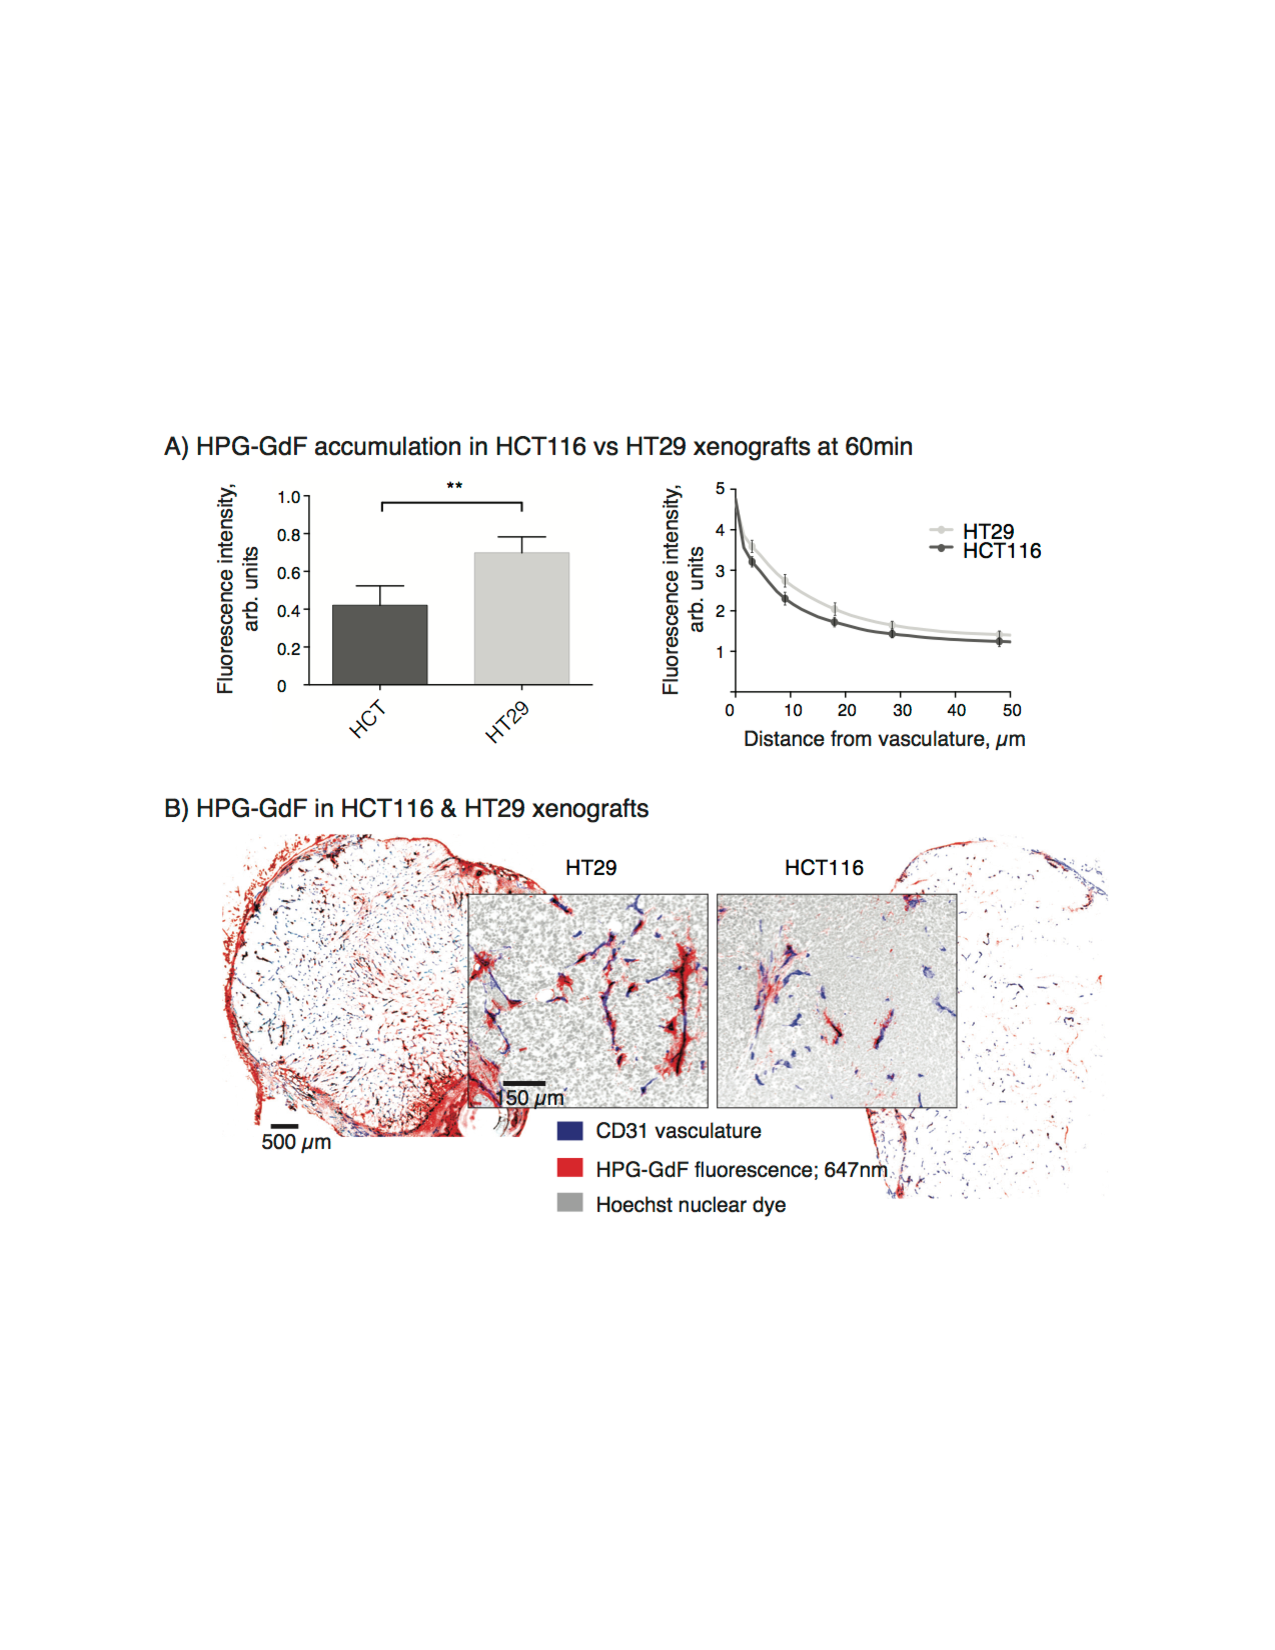
\includegraphics[width=\textwidth]{hpg/hpg-paper1-images/hpg_fig6-accumulation.pdf}
 \caption{HPG-GdF distribution in HCT116 and HT29 colorectal tumour xenografts at 60 min: histological analysis.
 (A) The whole-slice average fluorescence intensity shows that HPG-GdF accumulates to a greater degree and distributes further away from vasculature in HT29 tumours.
 (B) Sample images show HPG-GdF (red) overlaid on CD31 (blue); insets also display nuclear density (grey).
 A greater degree of HPG-GdF accumulation can easily be appreciated in the HT29 tumours.}
 \label{hpgpaper1:fig6}
 \end{center}
\end{figure}

However, an MR-measured difference between HCT116 and HT29 vascular function was seen with the BAT data for HPGGdF, as the fraction of enhancing voxels was significantly lower in the HCT116 relative to the HT29 tumours (BAT-EV for HPGGdF in HCT116 was 52.2 $\pm$ 4.8\% and that in HT29 was 81.8 $\pm$ 5.0\%, p < 0.05*) (Table 3).
This corresponded to the histological data, which also shows HCT116 tumours as having a greater proportion of necrotic tissue (necrosis fraction for HCT116 was 52.4$\pm$3.6\% versus 37.7$\pm$5.1\% in HT29, p<0.05*).
Of the HPGGdF BAT-enhancing voxels, the averaged fPV and aPS parameters were also determined (Table 3), and no difference was seen with the plasma volume between tumour models (fractional fPV for HCT116 is 2.67 $\pm$ 0.33 x 10$^{-1}$4 and that for HT29 is 2.16 $\pm$ 0.27 x 10$^{-1}$4, p > 0.05), but a trend of greater aPS was seen in the HT29 xenografts (aPS for HCT116 was 2.38 $\pm$ 1.00 x 10$^{-1}$8 and that for HT29 was 5.81 $\pm$ 1.4 x 10$^{-1}$8, p = 0.056*).
aPS of HPGGdF was the only MR-derived biomarker able to detect the significant difference in vascular function between these two tumour models.
Complete data sets for HCT116 tumours are shown in Fig.~\ref{hpgpaper1:fig7}.

\section{Discussion}

The use of MCAs for imaging and describing tumour vascular function is a widely pursued area of research.
Many studies have investigated a range of sizes, where smaller molecules extravasate and distribute through tissue too quickly to be considered as sensitive blood pool agents, and larger molecules often accumulate too slowly for adequate signal detection~\cite{Kyle:2007ch,Tang:2013fi,Sourbron:2011ce}.
In this work we describe HPG-GdF as an MR-visible MCA of 583 kDa, for which we have derived useful biomarkers that have sensitivity in measuring vascular function.
While the signal-to-noise from HPG-GdF concentration-time curves is not adequate to fit a complex pharmacokinetic model to determine parameters such as v$_p$, v$_e$ and K$^{trans}$, enhancement was measurable in most tumour voxels.
The number of Gd chelates on the HPG-GdF is approximately 300 per carrier molecule, which is high relative to many albumin chelates, the most common MCA in preclinical use, which typically have about 20 chelates per carrier~\cite{Ogan:1987tg}.
In addition to a greater number of Gd per carrier, the HPG-GdF accumulates in the perivascular space and fails to distribute more than a few micrometers from most vessels within a short DCE imaging timeframe (Fig.~\ref{hpgpaper1:fig3}).
This accumulation could provide a greater concentration for detection of a local, permeable tumour vessel and avoids the risk of conflating this with the distribution and accumulation elsewhere in tumours.
These attributes of HPG-GdF may make it more sensitive and more specific than a smaller MCA such as albumin-Gd-DTPA.
A minimum DCE imaging time from the presented data would appear to be about 15 min for the analyses described, which is longer than the suggested 5min ideal for practical clinical utility~\cite{Turetschek:2004bw}.
It is possible that greater signal could also be obtained by decreasing the time resolution from the 2.4s used in these studies, since HPG-GdF remains largely intravascular.
HPG-GdF contains the Gd-DOTA complex, which is highly thermodynamically stable and kinetically inert.
The dissociation constant for Gd-DOTA (log K = 24.7) is much higher than those for CaDOTA (log K = 17.23) or Mg-DOTA (log K = 11.92), hence neither Ca nor Mg can transmetallate Gd from the Gd-DOTA complex~\cite{Baranyai:2005ta}.
Biodegradation of HPG-GdF is therefore likely minimal, occurring through enzymatic attack of the end group, similar to that seen for polyethylene glycol~\cite{Kawai:2002fc}.
However, the long half-life and relatively slow excretion of HPGs through the reticuloendothelial system of the liver suggest that the potential for toxicity should be investigated and monitored.
A biodegradable version of HPG has recently been synthesized and might circumvent these potential concerns, and will be a focus in future DCE studies investigating the use of HPGs as MR-visible MCAs~\cite{Shenoi:2013id}.
Limited extravasation of HPG-GdF is likely due to the selective permeability of tumour vessels with adequate pore sizes for passage of the bulky molecule, a phenomenon described as the enhanced permeability and retention (EPR) effect~\cite{Maeda:2013hq}.
Limited distribution through the interstitium is also most probably the result of its significant size.
We have observed HPG-GdF to be much more restricted in its distribution than is suggested by the diffusion coefficients (D(HPG) = 3.7 x 10$^{-1}$7 cm$^2$ s$^{-1}$1 and D(Gadovist) = 3.6 x 10$^{-1}$6 cm$^2$ s$^{-1}$1), as the larger agent reaches only 10-15$\mu$m away from vessels within an hour whereas Gadovist reaches all areas of a tumour.
HPG-GdF molecules experience greater obstacles to their movement through the heterogeneous tumour microenvironment due to their size, but also possibly due to steric hindrances, non-specific binding or sequestration~\cite{Minchinton:2006gs}.
The large size of HPG-GdF is a significant advantage.
An approximately exponential increase in sensitivity for detection of permeability has been reported with increasing MCA size (19).
If extravasation of HPG-GdF only occurs in vessels that are permeable, and the agent does not distribute through the extravascular space to distances away from vessels, then MR-visible HPG-GdF enhancement suggests the presence of vasculature, and accumulation of the agent over time indicates the local presence of a hyperpermeable vessel.

\begin{figure}[htbp]
 \begin{center}
 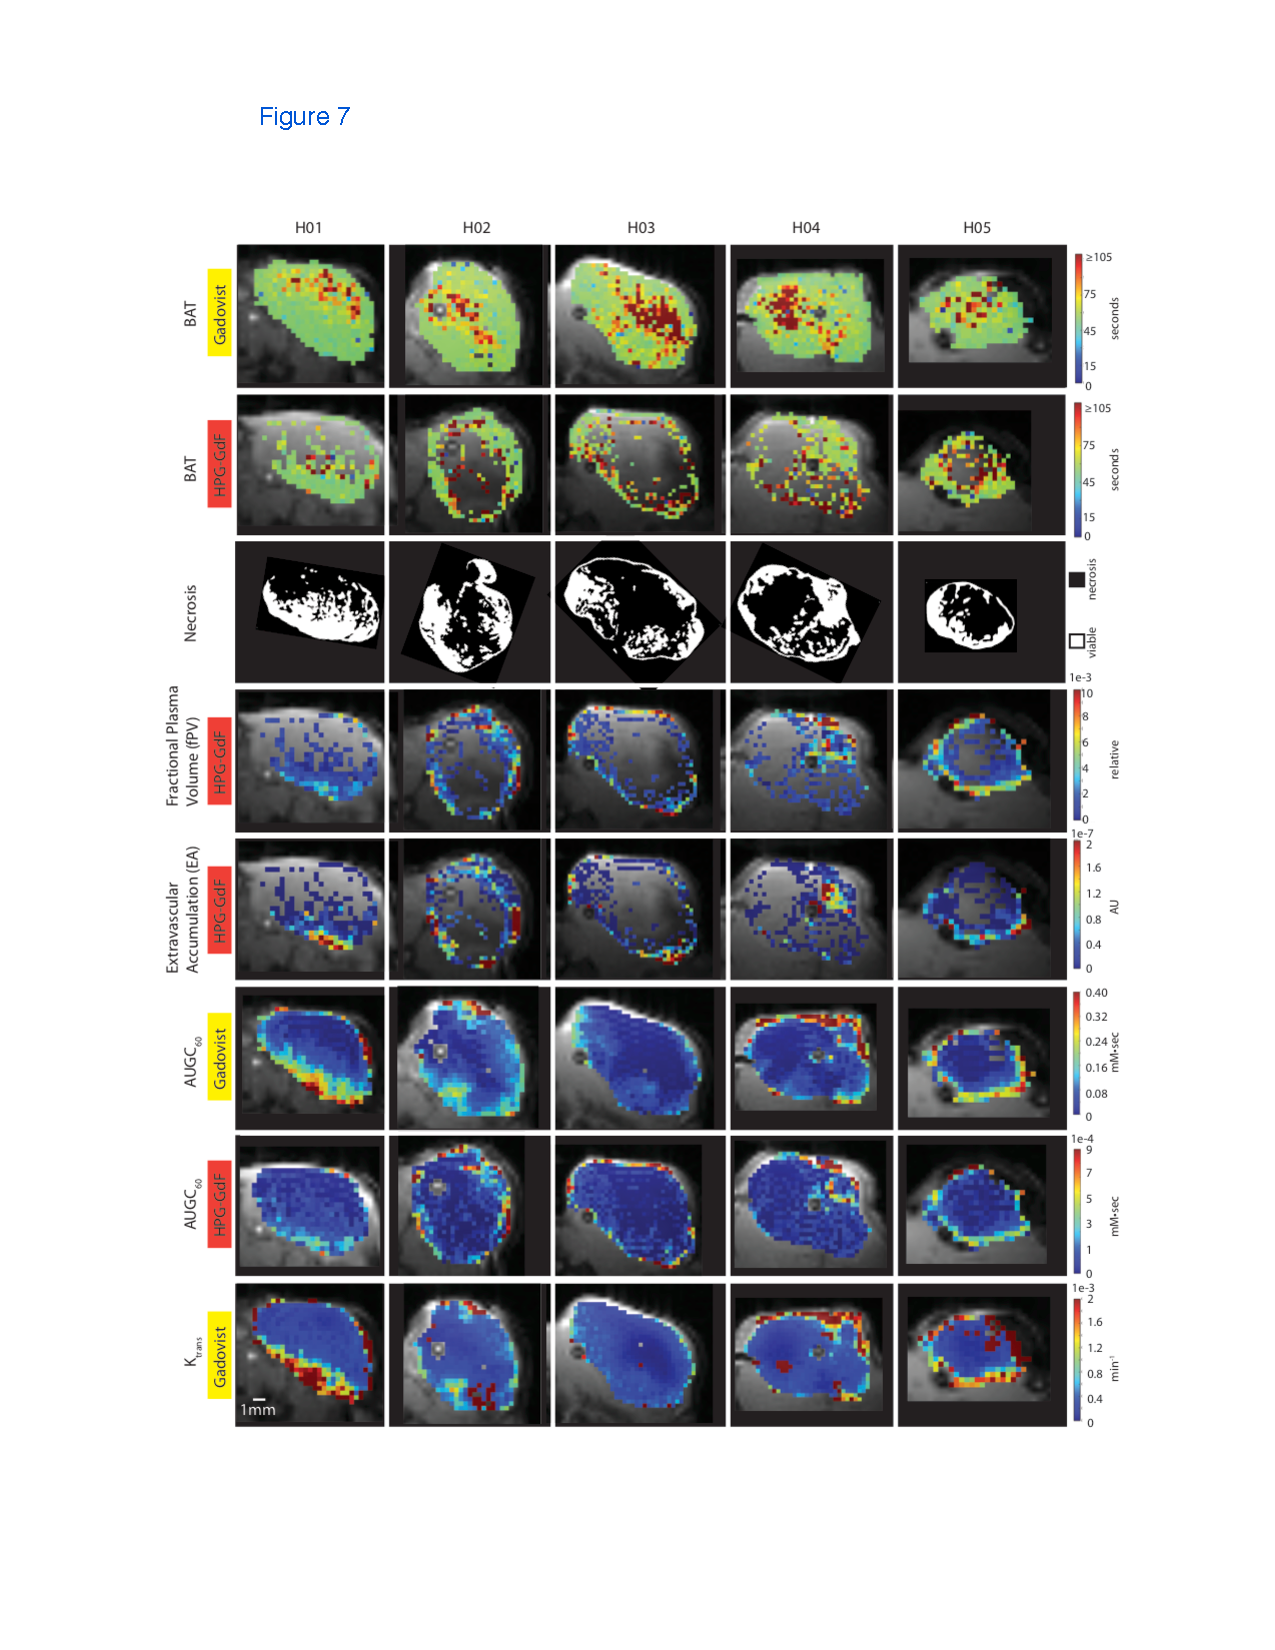
\includegraphics[width=0.8\textwidth]{hpg/hpg-paper1-images/hpg_fig7-hct116.pdf}
 \caption{Vascular function in HCT116 xenografts. Whole-slice maps are presented for individual HCT116 tumours (T01-T05, vertical columns) for parameters derived from MR imaging of Gadovist (BAT, AUGC60, K$^{trans}$), MR imaging of HPG-GdF (BAT, fPv, aPS, AUGC60) and histological imaging (necrosis).}
 \label{hpgpaper1:fig7}
 \end{center}
\end{figure}

A typical enhancement curve for HPG-GdF is shown in Fig.~\ref{hpgpaper1:fig2}.
The size of the initial step-like enhancement is interpreted as the fPV, and the slope of signal change for the remaining enhancement is reported as the aPS, reflecting the extravascular accumulation of HPG-GdF (Fig.~\ref{hpgpaper1:fig2}).
These parameters are not correlated with each other, with either value potentially significantly higher or lower than the other in the same voxels (Fig.~\ref{hpgpaper1:fig5}).
A pattern of faster enhancement at the tumour margins is consistent for both contrast agents, and, while Gadovist eventually arrives in all the tissue, including regions of necrosis, many voxels that correspond to necrotic regions fail to enhance with HPG-GdF within the 37 min imaging session.
We found that HPG-GdF BAT-enhancing voxels correspond to areas without necrosis: see Figs.~\ref{hpgpaper1:fig4} and ~\ref{hpgpaper1:fig7} for parameter maps of all BAT-enhancing voxels compared with histologically validated necrotic regions.
Therefore, we identified perfused regions of tumour tissue for further vascular function analysis using the straightforward approach of selecting voxels that had positive BATs for their HPG-GdF enhancement curves.
Selection of viable tissue and the exclusion of necrotic tissue is a desirable approach for controlling for inter-tumour heterogeneity, since MRI data is most often described as a whole-tumour average.
In the event that different tumours possess variable necrotic burdens, or if the necrotic fraction increases over time with treatment, selective analysis of viable tissue can control for this variability.
Qualitative comparisons of well-matched, whole-slice images from multiple modalities emphasize the utility of screening for BAT-enhancing voxels to select for perfused and viable tissues.

Without this information analysis may be restricted to regions of tissues at the tumour margins where hot spots of vascularization are observed histologically, and tissue is assumed to be viable in the MR image~\cite{Pathak:2005gu,Li:2005gw}.
In the colorectal xenografts examined here the amount of necrosis varied considerably, and, while it is typically located more in the core than the tumour margins, there is substantial inter-tumour heterogeneity with respect to the amount and location of necrosis.
Notably, while the values for K$^{trans}$(Gadovist) are on average higher around the entire tumour rim, the fPV and aPS values are more heterogeneously arranged around the rim and within the interior of the tumour.
Our more comprehensive approach, validated by observations of viable tissue and perfused vessels within tumour interiors in histological sections, is a significant improvement over selectively assessing limited regions or hotspots for histological or MR quantitative analysis.
Traditional DCE-derived parameters such as AUC and K$^{trans}$ are composite measures influenced to varying degrees by vascular surface area, permeability and blood flow.
Our histological data supports a significant range in the propensity for HPG-GdF to extravasate, suggesting that assumptions of perfusion or permeability-limited conditions are not applicable to all areas of the tumour microenvironment.
Hence, we cannot conclude that aPS is exclusively proportional to permeability-surface area (PS) in the whole microenvironment.
For example, although the amount of HPG-GdF leaking into the extravascular space is dependent on the vessel being permeable to large molecules, the amount of accumulation, and therefore the amount of signal enhancement, may still be impacted by the concentration of contrast agent within the vessel.
Longitudinal gradients can occur locally in permeable vessels as the contrast agent leaks out, despite plasma concentrations remaining consistent in overall systemic circulation~\cite{Erickson:2003wt,Dewhirst:1999jh}.
Thus, the aPS is a measure of vascular function that has contributions from permeability as well as, when permeability is very high, perfusion.
These limitations in the physiological interpretation of aPS are similar to those that apply to K$_{trans}$ and AUC for all contrast-enhanced modelling.
Parameters that are based on the amount and proportion of contrast agent enhancement are dependent on fewer assumptions than are pharmacokinetic model-derived parameters such as K$^{trans}$.
Biophysical signals are dependent on the many variables necessarily involved in obtaining MR images, such as the scanner, imaging sequence, RF coil and analysis techniques.
Interpreting magnitudes of change in highly variable tumours may be more reliable than assuming invariable pharmacokinetic attributes or unchanging tumour microenvironments, and may make simplified biomarkers such as fPV and aPS more applicable to clinical studies conducted across multiple centres~\cite{OConnor:2012ie}

\section{Conclusion}

HPG-GdF is a largely intravascular MCA that selectively extravasates from hyperpermeable tumour vessels, accumulating in the perivascular regions without distributing through the tumour interstitium.
The high concentration of Gd chelates per carrier molecule in combination with its excellent solubility makes HPG-GdF detection possible despite the relatively low plasma fraction within tumours.
By carefully comparing the vessel parameters of small and large molecule contrast agents in the same tumour, as well as comprehensively assessing the location of MCA within the tumour relative to vasculature and necrosis, we conclude that BAT, fPV and aPS biomarkers derived from HPG-GdF enhancement provide a sensitive and specific approach to measuring tumour vascular function.
HPG-GdF and these analysis techniques would be appropriate in the evaluation of tumour angiogenesis and response to treatment for preclinical research, with potential for eventual translation to the clinic.


\endinput

%% The following is a directive for TeXShop to indicate the main file
%%!TEX root = ../diss.tex

\chapter{Oxygen enhanced MRI}
\label{ch:oemri}

\section{Preface}

Stuff about contributions 

% ======================================================================
\section{Introduction}
% ======================================================================

Hypoxia is a well-established component of the tumor microenvironment, arising most often as tumor cell proliferation outpaces the growth of new vasculature.
Tumor hypoxia is an indicator of poor prognosis and is responsible for tumor resistance to radiotherapy and some chemotherapies, but is also a potentially useful target for novel anti-cancer drugs~\cite{Wilson:2011jp}.
Assessing tumor hypoxia in the clinical setting is challenging largely due to the invasive nature of biopsy-dependent techniques and the limited capacity and high expense of the more favored, non-invasive PET imaging of hypoxia tracers~\cite{Horsman:2012kw}.
The utility of screening patients for hypoxia was demonstrated retrospectively in trials of the hypoxic cytotoxin tirapazamine, where those patients with greater PET-imaged hypoxia experienced greater benefit ~\cite{Rischin:2006fz}.
However, subsequent trials of drugs targeting hypoxia, including those for evofosfamide that failed to show clinical benefit, have not used hypoxia imaging to stratify patients.
A practical, widely applicable, and non-invasive imaging method is urgently required as a biomarker to monitor tumor hypoxia in many contexts, and is crucial to the development and clinical evaluation of future hypoxia-targeting drugs.

The T$_1$ shortening property of oxygen dissolved in fluid has been known since 1955~\cite{Chiarotti:1955kf} and pioneering work by Young et al. showed that oxygen acts as a paramagnetic contrast agent by demonstrating its ability to reduce T$_1$ upon inhalation~\cite{Young:1981vf}. 
Inhalation of 100\% oxygen has also been shown to elicit strong T$_1$ effects in the kidney\cite{Jones:2002dh}, spleen\cite{Tadamura:1997vc} and the poorly oxygenated retina~\cite{Berkowitz:2001uz}. 
Subsequent oxygen-enhanced MRI (OE-MRI) efforts have included either acquisition of quantitative T$_1$ maps before and after oxygen breathing, or acquiring dynamic T$_1$-weighted (T1W) signal intensity images and calculating $\Delta$T$_1$ during periods of oxygen inhalation.
The subtle but measurable influence of tissue oxygenation on T$_1$ in tumors has been reported by O'Connor~\cite{OConnor:2016ee,OConnor:2009ku,OConnor:2009bp,Little:2018iu}, Mason~\cite{Zhao:2015ez,White:2016fz,Hallac:2014cb}, Gallez~\cite{Jordan:2012do}, and others~\cite{Tadamura:1997vc,McGrath:2008kx,Kershaw:2010ha,Linnik:2013hf}. 
However, due to the changes in T$_1$ that arise as oxygen dissolves in the plasma and interstitial fluid being quite small, T$_1$ maps have poor sensitivity and application of OE-MRI techniques in cancer has yielded mixed success.
OE-MRI continues to suffer from low SNR and it has not found routine clinical use largely because isolating small signal changes due to dissolved O$_2$ is a challenge~\cite{OConnor:2016ee, Zhao:2015ez}.

Typical imaging times for existing OE-MRI methods range from 20-45 minutes often making it impractical for easy inclusion in experimental protocols. 
An MRI technique measuring tumor oxygenation that is sensitive, fast, flexible, repeatable, and non-invasive has the potential to significantly impact the clinical fields of radiation biology and hypoxia drug targeting.
In this study, we present a new dynamic OE-MRI (dOE-MRI) method that allows extraction of very small dynamic signal changes in T$_1$W images by inducing step changes in the inspired oxygen through a repeated, cycling gas challenge.
To isolate the signal component that matches cycling gas, a machine-learning approach called independent component analysis (ICA) is used to analyze MR images as first proposed by McKeown at al~\cite{McKeown:1998wo}.
ICA is a form of blind source separation algorithm that separates the additive signals on the basis of the statistical independence of individual components~\cite{Hyvarinen:2000vk}.
With the application of a cycling oxygen challenge and processing the data using ICA, our dOE-MRI approach represents a significant improvement in the sensitivity and application of MRI for measuring tumor oxygenation, making it more practical for wide application.
% ======================================================================
\section{Methods}
% ======================================================================
\subsection{Mice and tumors}

All animal experimental procedures were carried out in compliance with the guidelines of the Canadian Council for Animal Care and were approved by the institutional Animal Care Committee. 
Female NRG mice were implanted with murine squamous cell carcinoma SCCVII tumors (5 x 10$^5 $cells in 50 $\mu$l serum-free media; cells provided by Dr. J Evans) or with human colorectal carcinoma HCT-116, human ovarian carcinoma SKOV3 or human breast carcinoma BT-474 tumors (each as 10 x 10$^6 $cells in 50 $\mu$l serum-free media; cell lines obtained from the American Type Culture Collection) and were imaged when the largest tumor diameters reached approximately 8-10 mm.
Mice were anesthetized with isoflurane for the duration of imaging sessions until euthanasia, and were positioned supine on the custom surface coil apparatus.
Throughout the imaging session, a small animal monitoring system (SAII Instruments, Stony Brook, NY, USA) was used to monitor respiration rate, varying between 80-100 breaths per minute, and body temperature, maintained at 36.8 $\pm$ 0.5$^\circ$C using a continuous airflow heater.
All animals were injected with 60 mg/kg pimonidazole hydrochloride (HypoxyProbe) 30 min prior to imaging to label hypoxic cells and were euthanized within 15 min of imaging completion.
Tumors were embedded and frozen in optimum cutting temperature medium (OCT; Tissue-TEK).

\subsection{Immunohistochemistry, image acquisition and analysis}
Co-planar MRI slices and histological sections were obtained by imaging perpendicular to the longest tumor axis in MRI and serial-step 10 $\mu m$ cryosections were cut at 0.5-mm intervals in the same plane.
Slides were then fixed in acetone-methanol for 10 min and whole sections were immunohistochemically stained~\cite{Kalra:2017is} for CD31 (PECAM; visualized using secondaries labeled with Alexa 647nm) to label blood vessels, and for pimonidazole (HypoxyProbe-1; visualized using secondary labeled with Alexa 546nm) to label hypoxic cells. Sections were then stained using Hoechst 33342 (bisbenzimide) to label all cell nuclei.
Whole-tumor sections were imaged using a robotic fluorescence microscope (Zeiss Axioimager Z1), a cooled, monochrome CCD camera (Retiga 4000R; QImaging), a motorized slide loader and x-y stage (Ludl Electronic Products) and customized ImageJ software~\cite{Collins:2007jr}. 
Adjacent microscope fields of view were tiled such that images of entire tumor cryosections were captured at a resolution of 1.5 $\mu m$/pixel. 
Using anatomical landmarks and accumulated thicknesses of serial-step sections as estimates of distances from the edges of whole tumors, sections were chosen to match the MR slices. 
ImageJ and user-supplied algorithms were used to super impose digital images which were then manually cropped to tumor tissue boundaries with staining artifacts removed. A threshold was applied to images to identify positive pimonidazole staining, and the number of positive pixels was determined as a percentage of the total number of pixels in the tumor image. The histological hypoxic fraction is reported in the highly necrotic HCT-116 tumours as the percentage of pimonidazole+ pixels summed with the percentage of necrotic pixels, as this value should most closely approximate the MR imaging data that does not discriminate between these regions; SCCVII tumours do not have necrosis and so the same value is reported as the percentage of pimonidazole+ pixels.
Overlaid greyscale images were converted to false color for visualization with pimonidazole as green and CD31 as magenta. 

\subsection{MRI Data Acquisition}
All MRI experiments were performed at the UBC MRI Research Centre on a 7T Bruker BioSpec 70/30 scanner at room temperature with a volume transmit coil and custom surface receive coil.
Each imaging session began with pilot axial and coronal T$_2$W scans for tumor localization and slice prescription.
Eight contiguous axial slices (1mm thickness) were acquired with an in-plane field of view of 3.84 cm x 1.92 cm and a matrix size of 128 x 64.
Dynamic oxygen enhanced MRI (dOE-MRI) scans were acquired with a 2D multi-slice FLASH-based sequence with TE/TR = 2.67ms/66.7 ms, $\alpha$ = 40$^\circ$, temporal resolution of 4.3s with 198 repetitions for a total scan time of about 14 minutes.
The spatial resolution and geometry for all scans in the imaging session were matched and an experienced operator outlined the tumor on each slice of the anatomy MR images to construct the region of interest (ROI) for each animal.

\noindent\textbf{Gas challenge during MRI:} Tumor-bearing mice began the dOE-MRI gas challenge breathing medical air and were switched between 100\% oxygen and medical air in two-minute intervals.
This paradigm continued for three cycles over a total of fourteen minutes; gases were switched manually and each switch took about five seconds to complete.

\subsection{MRI Data Analysis}
\textbf{dOE-MRI maps:} A suite of in-house software was developed using the python machine learning library scikit-learn~\cite{Pedregosa:2011tv}, specifically \texttt{sklearn.decomposition.FastICA} based on the technique described by Hyvarinen~\cite{Hyvarinen:2000vk}.
The FastICA algorithm is applied to serially acquired T$_1$W images and the output is a paired set of components and weighting factors for each voxel in the dataset.
Extracted independent components are not ordered and while the component selection can be automated, in this study an observer was assigned to select the appropriate component (Figure~\ref{technique}).
The number of independent components for each imaging session was chosen by the operator and ranged from 4-9 to ensure the cyclic behavior of the T$_1$W signal intensity corresponding to the gas challenge appeared in only one component. 
The dOE-MRI maps were obtained by dividing the ICA weighting-factor maps by the mean signal-intensity maps to obtain a spatial map for the strength of a particular voxel's contribution to the component of interest ($c_4$ in Figure~\ref{technique}).
In these dOE-MRI maps, voxels are colored to indicate the amount by which a given pixel intensity timecourse is modulated by the oxygen-related component.  
The green-white-purple color spectrum depicts the degree to which voxels respond to the cycled gas challenge.
Purple indicates O$_2$-positive voxels whose timecourse exhibits a higher and more positive contribution from the corresponding ICA component, representing an increase in T$_1$W signal intensity in response to the supplied 100 \% oxygen, and corresponding to areas with excess dissolved oxygen. 
O$_2$-negative voxels that show a decrease in T$_1$W signal intensity with a negative contribution from the corresponding ICA component under 100 \% oxygen breathing are depicted as green. 
Regions whose T$_1$W signal intensity timecourses responds only weakly or not at all to the gas challenge are shown in white hues.
Fraction of voxels that are negative on dOE-MRI maps were correlated with the histological hypoxic fraction using Pearson's r.

\noindent\textbf{OE-MRI without ICA:} To assess whether or not ICA was necessary to create oxygenation maps, the MR signal intensity data was correlated with two modeled paradigms: 1) a square wave which corresponds to the concentration of delivered oxygen; 2) a synthetic hemodynamic response function (HDRF) created by convolving a square wave with an exponential ($\tau=0.32$ms).
Correlations were calculated voxel by voxel using:

\begin{equation}
r = \frac{\Sigma^n_{i=1} (x_i - \bar{x}) (y_i - \bar{y})}{\sqrt{\Sigma^n_{i=1} (x_i - \bar{x})^2 \Sigma^n_{i=1} (y_i - \bar{y})^2}}
\end{equation}
where $x$ is the model paradigm and $y$ is the T$_1$W signal intensity timecourse.
The resulting correlation maps are estimates of the strength of the input paradigms with the acquired signal intensity.

% ======================================================================
\section{Results}
% ======================================================================

\subsection{ICA isolates small changes in T$_1$W signal intensity}

An example signal intensity vs.\ time curve is shown for a whole slice ROI compared with a single voxel (Figure~\ref{technique}B).
A mean signal intensity increase is seen for both the whole slice and the individual voxel during each of the oxygen periods of the cycle, however the magnitude of $\Delta SI$ for the individual voxel is about 10\% and the noise is of the same order of magnitude.
The slice-averaged timecourse has much less noise compared to the individual voxel, but the size of the effect is also reduced and the contrast to noise is similarly poor.
ICA was then applied to the same dataset and in this example, four independent components were extracted (Figure~\ref{technique}C). 
Each individual independent component is scaled such that its norm is one ($||c_i||=1, \forall i $).
Corrupting influences are often present such as temperature drifts yield slowly increasing or decreasing trends (for e.g., $c_1$), artefacts resulting from slight sub-pixel motion near the edges of the tumor ($c_2$) and breathing artefacts corresponding to short-lived spikes ($c_3$).
Only one extracted component follows the step function of the oxygen challenge and positively identifies an effect of oxygen breathing (c$_4$).
\begin{figure}[htbp]
   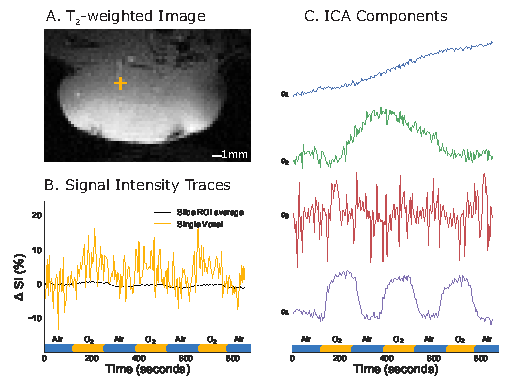
\includegraphics[width=0.5\textwidth]{oemri/oemri-images/fig1_technique.pdf} % requires the graphicx package
   \caption{(A) T$_2$W MRI of a tumor xenograft at 7T and (B) the corresponding T$_1$W signal-time traces of a single voxel (solid yellow) and whole-tumor slice ROI (dotted black) during gas cycling at two-minute intervals of air (x axis; blue) and O$_2$ (x axis;yellow).
(C) Plot of the four extracted ICA components from the entire tumor ROI, component \textbf{$c_4$} (purple) exhibits the same temporal features as the oxygen cycling time course shown along the bottom. All components are normalized, no vertical scale is shown.}
   \label{technique}
\end{figure}

\subsection{ICA enabled dOE-MRI detects variable oxygenation in a range of tumor models}
Tumors of human and murine origin and comprising a variety of tumor microenvironments were imaged, including fast growing, highly vascularized murine squamous cell (SCCVII) and human ovarian carcinomas (SKOV3), slower growing and well vascularized human breast cancer (BT-474), as well as a relatively fast growing but more poorly vascularized human colon colorectal carcinoma (HCT-116).
The inter-model heterogeneity of the tumors is reflected in the mean fraction of negative voxels in the dOE-MRI maps, which were 46 $\pm$ 6\% for BT-474, 36$\pm$3\% for HCT-116, 31$\pm$5\% for SCCVII, and 14$\pm$4\% for SKOV3 tumors. 
Considerable intra-tumor heterogeneity is also observed within some models, particularly the BT474.
dOE-MRI maps representing the mean fraction of negative voxels are shown for each tumor type in Figure~\ref{versatile}.
\begin{figure}[htbp]
   \centering
   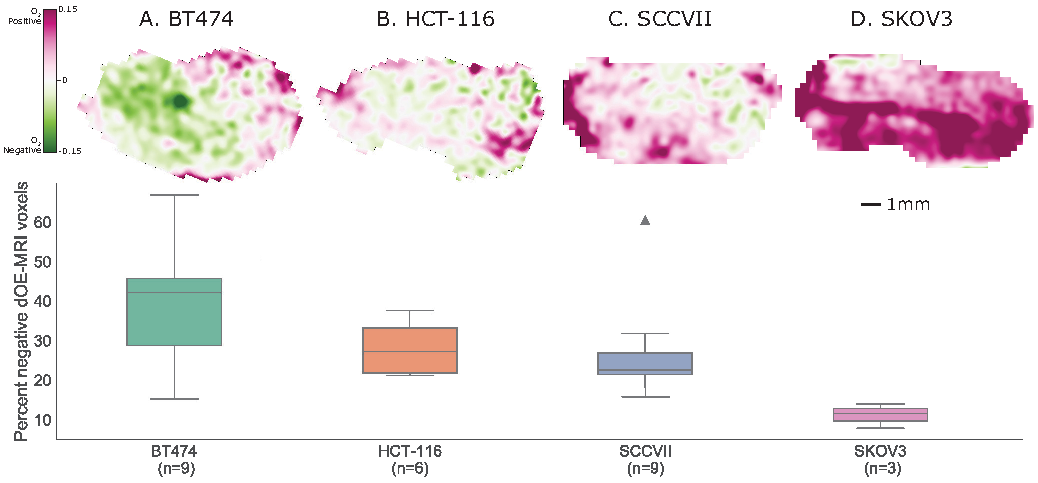
\includegraphics[width=\textwidth]{oemri/oemri-images/fig2_versatile.pdf} % requires the graphicx package
   \caption{Top: dOE-MRI maps for four tumor models HCT-116, BT-474, SCCVII, and SKOV3 are shown. Chosen slices are representative of the mean percent negative dOE-MRI fraction for the respective tumour model.
Bottom: The box-whisker plot shows the quartiles of percent negative dOE-MRI voxels for all imaged tumours.
\label{versatile}}
\end{figure}

\subsection{dOE-MRI with ICA does not require assumption of a response function}
To determine whether dOE-MRI maps obtained with a model-free ICA approach (Figure~\ref{fig_correlation}A) are comparable to maps assuming a mathematical model of the response, alternative oxygenation status maps were constructed. 
In Figure~\ref{fig_correlation}B and C, two example mathematical models - a square wave and the estimated hemodynamic response function (HDRF) - are correlated to the voxel-by-voxel raw time signal. 
Regions most correlated with the input paradigm remained purple in both alternative maps generated from modeled response functions.
Particularly when using the HDRF, the alternative oxygenation map showed very similar patterns in the regions demarcated as O$_2$-positive and O$_2$-negative. 
However, the map generated from correlating a square wave led to consistent underestimation of oxygenation relative to the model-free dOE-MRI map.

\begin{figure}[htbp]
   \centering
   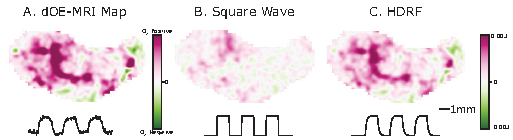
\includegraphics[width=\textwidth]{oemri/oemri-images/fig3_correlation.pdf} % requires the graphicx package
   \caption{(A) dOE-MRI map of an SCCVII tumor where purple voxels contribute strongly to the extracted component using ICA in the T$_1$W signal timecourses. 
Green voxels in the dOE-MRI map have a strong contribution of the inverse extracted component. Pearson's r-maps are shown correlating the raw time-signal voxel by voxel with a square wave (B), and an exponential convoluted with a square wave called the hemodynamic response function (HDRF) (C).
   \label{fig_correlation}}
\end{figure}
\subsection{Variability of response in individual oxygen cycles}

A full dOE-MRI sequence involved three cycles of oxygen but to assess the potential for shortening the sequence we also separately applied ICA to each of the three oxygen cycles independently.
Separate dOE-MRI maps, as well as voxel-wise correlation plots of a representative SCCVII tumor, are shown in Figure~\ref{fig_repeatability} with Pearson's r$_{all-1}$=0.74,r$_{all-2}$=0.86,r$_{all-3}$=0.84.
Pearson's r ranged from 0.79 to 0.87 for a similar analysis in a representative HCT-116 tumor.

The stability of the independent component extraction was assessed by undersampling the full timecourse threefold prior to application of ICA, and a high correlation between the dOE-MRI maps from full and three-fold undersampled timecourses is observed (Figure~\ref{fig_repeatability}E; Pearson's r = 0.84). 

\begin{figure}[htbp]
   \centering
   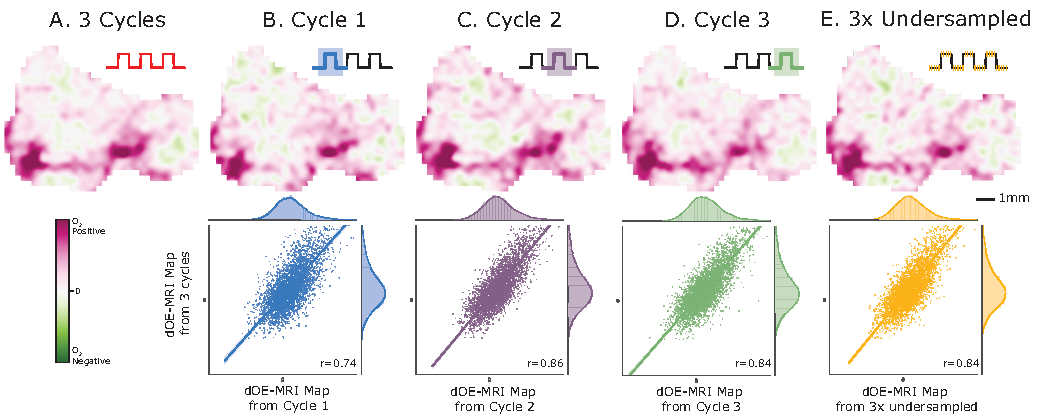
\includegraphics[width=\textwidth]{oemri/oemri-images/fig4_repeatability.pdf} % requires the graphicx package
   \caption{The dOE-MRI map including the full dataset of all three cycles (A) is compared to each of the three gas cycles separately (B,C,D), and to a map that temporally undersamples by selecting every third datapoint from the full dataset (E).
Voxel-wise plots of each map are correlated to the full dataset and a linear regression with Pearson's r is shown.
   \label{fig_repeatability}}
\end{figure}
\subsection{dOE-MRI maps correspond to matched histology sections}

Tumor tissue cryosections obtained to match MR imaging slices were stained for vasculature (CD31) and regions of pimonidazole-labeled hypoxia and are compared side-by-side; Figures~\ref{fig_sccvii} and~\ref{fig_hct116} provide five examples for each of SCCVII and HCT-116 tumor models for detailed review.
Generally, in corresponding dOE-MRI maps for both tumor models O$_2$-positive voxels align with the most oxygenated regions of histology sections, where pimonidazole labeling is absent, however many areas of mismatch are also observed. 
More consistent is that O$_2$-positive voxels do not typically correspond to tissues identified as hypoxic in the histology sections (i.e. labeled with pimonidazole).
In general, the more necrotic HCT-116 tumours have fewer oxygenated (O$_2$-positive) regions and significantly more hypoxic (O$_2$-negative) regions in the dOE-MRI maps, compared to the SCCVII tumors that have no necrosis. 
Pimonidazole labeling is heterogeneously dispersed within regions of viable tissue containing tumor blood vessels for both SCCVII tumors, Figure~\ref{fig_sccvii}, and HCT-116 tumors, which typically have greater amounts of necrosis, Figure~\ref{fig_hct116}.
Figure~\ref{histo_correlations} shows the fraction of negative dOE-MRI voxels correlated with the histological hypoxic fraction. 
For SCCVII tumours (n=9) there was an excellent correlation, with Pearson's r = 0.91 (\textit{p}=0.0016). 
However the correlation in the HCT-116 tumors (n=6) was poor, with r=0.13 (\textit{p}=0.81). 

\begin{figure}[htbp]
   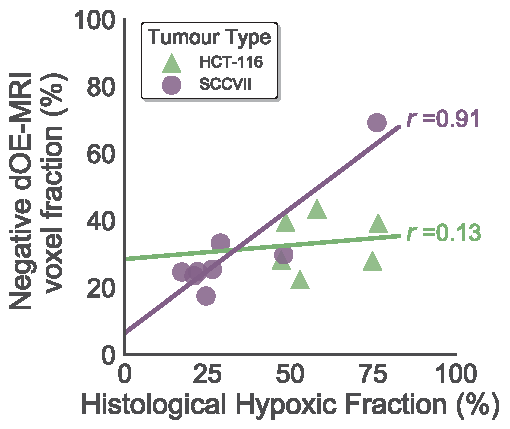
\includegraphics[width=0.5\textwidth]{oemri/oemri-images/fig5_histocorrelation.pdf} % requires the graphicx package
   \caption{The proportion of negative dOE-MRI voxels is plotted against the histological hypoxic fractions with Pearson's r = 0.91 for SCCVII tumours and r = 0.13 for HCT-116 tumours.
   \label{histo_correlations}}
\end{figure}

\begin{figure}[htbp]
   \centering
   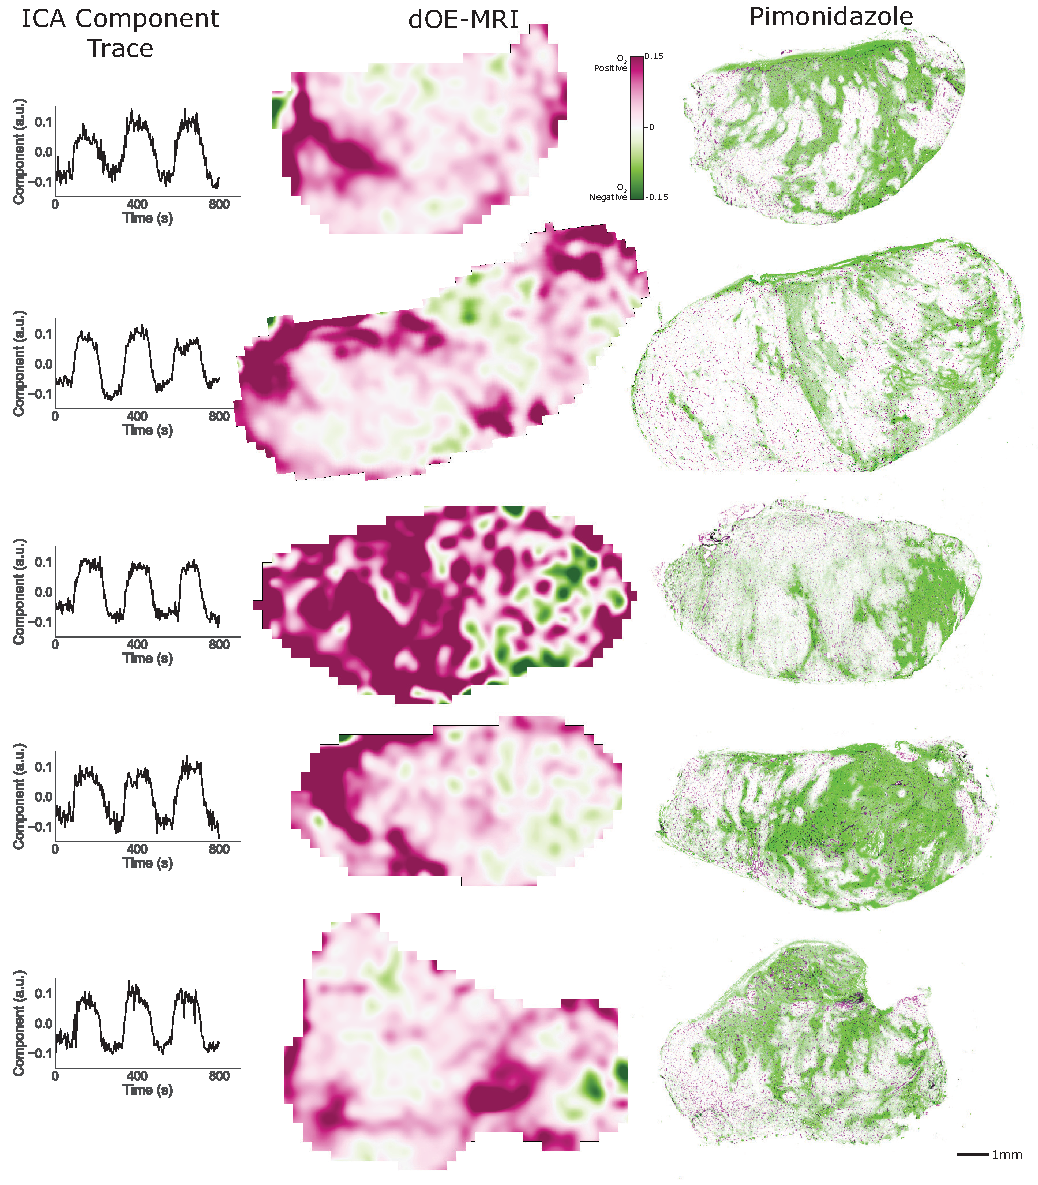
\includegraphics[width=0.9\textwidth]{oemri/oemri-images/fig6_sccvii.pdf} % requires the graphicx package
   \caption{SCCVII murine tumors with slice-matched histological images depicting pimonidazole-labeled hypoxia (green) and CD31-stained vasculature (purple) are shown next to the dOE-MRI parameter maps similarly colored with O$_2$-positive (purple) and O$_2$-negative (green) areas. Corresponding ICA extracted components are also shown.
   \label{fig_sccvii}}
\end{figure}
\begin{figure}[htbp]
   \centering
   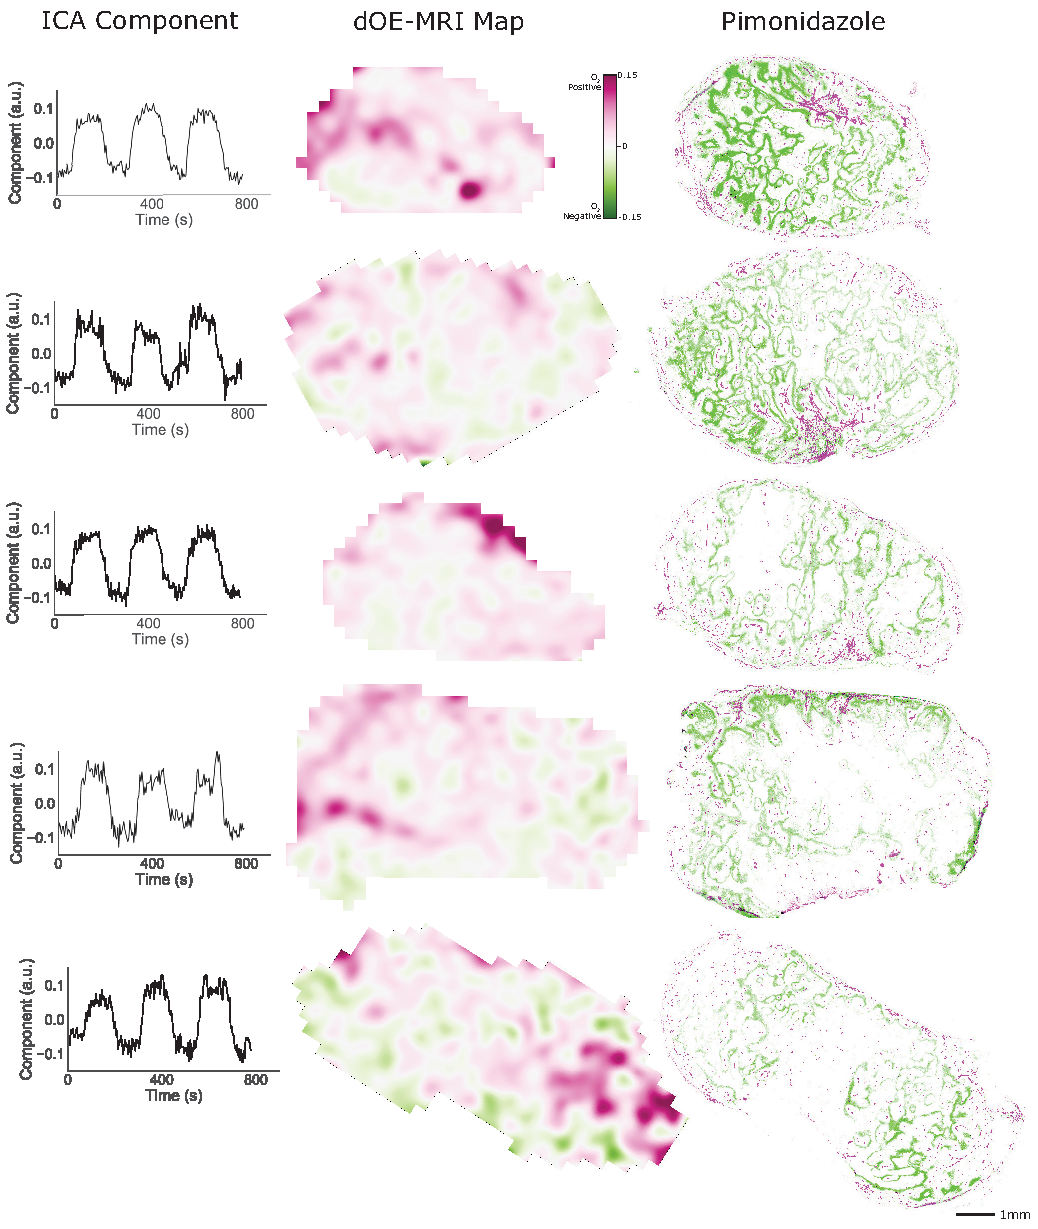
\includegraphics[width=0.9\textwidth]{oemri/oemri-images/fig7_hct116.pdf} % requires the graphicx package
   \caption{HCT-116 human colorectal xenografts with slice-matched histological images depicting pimonidazole-labeled hypoxia (green) and CD31-stained vasculature (purple) are shown next to the dOE-MRI parameter maps similarly colored with O$_2$-positive (purple) and O$_2$-negative (green) areas. Corresponding ICA extracted components are also shown.
   \label{fig_hct116}}
\end{figure}

%======================================================================
\section{Discussion}
% ======================================================================
Here we present an improved method for OE-MRI that employs two synergistic techniques to achieve higher speed and greater sensitivity.
First, a repeated gas challenge is used to probe tissue response by introducing an independent signal modulation unrelated to nuisance contributions such as temperature drifts and motion.
A repeating gas challenge improves the detection sensitivity of small amplitude signal changes that are typical of oxygen-enhanced MRI.
Second, a repeating signal modulation enables further improved sensitivity through the use of ICA, a signal processing technique to isolate source signals - T$_1$W changes due solely to the cycling oxygen - without knowledge of the tissue response (Figure~\ref{technique}).
While it is possible to generate correlation maps of the oxygen cycling paradigm with T$_1$W signal changes that appear very similar to dOE-MRI maps, an \emph{a-priori} assumption of a response function is required for this approach (Figure~\ref{fig_correlation}).
Furthermore, presupposing a particular oxygen response function biases the identification of responding O$_2$-positive voxels (Figure~\ref{fig_correlation}) underscoring the need for a model-free approach to extracting the oxygen-responding component.

The improved sensitivity of our technique results in broader applicability of dOE-MRI, as we found that an oxygen-enhancing component was extracted successfully in all imaged animals across a range of tumor models and environments (Figure~\ref{versatile}).
The unambiguous match of the identified component with the periods of the gas cycles increases the confidence that the small T$_1$W signal changes result from increased oxygen dissolved in the plasma and interstitial tissue fluids.
Maps from other extracted components (Supporting Information Figure S1) exhibit spatial patterns that could provide clues to the signal sources but associating meaning to them is challenging and would require additional data.
For example, even moderate shifts in temperature could drive a measurable change in T$_1$W signal during the timecourse, and a physiological monitoring system that is time-synced to the MR acquisition could illuminate this confounding variable. 
Nevertheless, we have established reliability of the technique by comparing maps from each cycle of the gas challenge to the map incorporating data from all three oxygen-cycles and have found no significant differences.
In fact, the strong correlations between dOE-MRI maps from each of the individual cycles of the gas challenge (Figure~\ref{fig_repeatability}) show that it is feasible to assess tissue oxygenation within 6 minutes.
Performing this analysis again with three-fold temporally under-sampled data suggests that there is sufficient SNR to successfully extract the oxygen responsive component (Figure~\ref{fig_repeatability}) with even a subset of the data. 

A limitation of OE-MRI is the difficulty in interpreting areas that do not show a reduction in T$_1$ as they may be either dead tissues that are \textit{unperfused and not oxygenated} or living, viable tissues that are \textit{perfused but not oxygenated} due to poor oxygen content of the supplying vessels. 
The latter population are of greater interest to the oncology community as it is these hypoxic but viable cells that have significant influence on treatment outcomes~\cite{Horsman:2016go}. 
The dOE-MRI technique presented here successfully correlates tumor oxygenation dOE-MRI and histology measures in SCCVII tumors but, despite improvements to sensitivity, a similar quantitative comparison in the HCT-116 tumor line showed poorer association (Fig.~\ref{histo_correlations}). 
This is likely attributable to the much higher amounts of necrosis typical of the HCT-116 model relative to SCCVII (Figs.~\ref{fig_sccvii} and \ref{fig_hct116}).
Mitigations to this limitation have been explored elsewhere and generally require a perfusion mask or $T_2^*$ - either technique can be added to the OE-MRI method proposed here to exclude necrosis and further improve sensitivity of the technique.

Application of existing OE-MRI techniques across a range of tumour models with varying perfusion characteristics has yielded mixed success without masking for perfused tissue.
For instance, O'Connor reported that in the highly perfused 786-0-R tumor lines, 85-96\% of all imaged tumor voxels were deemed to be oxygen-enhancing~\cite{OConnor:2016ee}.
In those tumors, there was a good correlation between histological hypoxic fraction and oxygen refractory voxels.
However, in the more weakly perfused SW620 tumors where only 76\% of the voxels are oxygen-enhancing, there were no significant correlations with the histological hypoxic fraction.
These issues were resolved by combining OE-MRI with DCE-MRI as a perfusion mask to select only perfused voxels for oxygenation assessment, thereby distinguishing between the viable hypoxic environment and necrotic dead tissues and improving the specificity and sensitivity of OE-MRI data. Using an IAUGC$_{60}$ map from DCE-MRI as a mask to obtain Oxy-R fractions O'Connor et al. showed good correlation with the histological hypoxic fraction~\cite{OConnor:2016ee}.
In more recent work, Little et al. showed oxygen enhancement in tumours with a histological hypoxic fraction as high as 43\%~\cite{Little:2018iu} and this translated very well to a study of six renal cell carcinoma patients.
Linnik et al. reported excellent correlation between percentage of ``negative AUC$_{OE}$'' ($O_2$-negative) voxels and percentage of hypoxic areas in the highly vascular preclinical U87MG tumor xenografts~\cite{Linnik:2013hf}.
A second approach for differentiating between viable but hypoxic regions and unperfused dead tissues, is to combine OE-MRI with $T_2^*$W acquisition and the BOLD effect to classify regions~\cite{Little:2018iu,Zhao:2015ez,White:2016fz,Burrell:2013je,Yang:2018vo} that show both effects. 
Excess oxygen in the blood will induce changes in Hb saturation, which alter the T2* resulting in a robust measure of areas with functioning vasculature. 
Conceivably, the saved acquisition time achieved with under-sampling T$_1$W dOE-MRI suggests that $T_2^*$W images could also be acquired to concurrently assess the blood oxygen level dependent (BOLD) response. 

Within the relatively short 14-minute imaging time, both the HCT-116 and SCCVII tumours show only minor changes in the oxygenation maps between cycles (Figure~\ref{fig_correlation}).
In longer imaging sessions, or during administration of an intervention, these same tumors may exhibit varying oxygenation patterns between cycles.
Periods of oxygen-starvation and re-oxygenation in tumors have been termed intermittent hypoxia and can arise due to temporary vessel occlusions~\cite{Dewhirst:2009de,Bayer:2011js}.
Recent work on measuring intermittent hypoxia in patients using R$_2^*$~\cite{Panek:2017ge} shows that interest in this phenomenon continues but the importance of intermittent hypoxia in tumors is unclear largely due to poor availability of techniques to measure it in the clinic~\cite{Michiels:2016hv}.
The relatively short imaging time for dOE-MRI makes assessing temporal oxygenation changes possible within a timescale on the order of minutes by comparing correlation maps generated from sequential cycles.

dOE-MRI offers a versatile technique where the duration of the cycles and gas challenge, temporal resolution and desired signal-to-noise can be modified based on the imaging objectives, which could include investigating intermittent perfusion or intervention-mediated changes in the tumor microenvironment. 
Of note, supplying excess oxygen to hypoxic tumor cells over time has the potential for increasing the baseline oxygen concentration, effectively reducing the hypoxic fraction and altering the tumor microenvironment~\cite{Linnik:2013hf}.
This would result in voxels becoming more oxygen responsive over progressive oxygen cycles and would depend on the tumor characteristics as well as the duration of the oxygen challenge.
This was not observed on the time scales in our study when using ICA to extract changes in T$_1$W signal intensity just due to the gas challenge. 
Should it arise in other contexts it could possibly be mitigated by extending the air-breathing part of the cycle, or by extracting that as a separate component using ICA.
The potential for creating a hyperoxia steady state by modulating oxygen duration is discussed further by Losert et al ~\cite{Losert:2002gt}.

Typically, histological validation of MR data is done by collapsing rich histology data into a single metric, such as a hypoxic fraction, with whole-tumor or single-slice average comparisons.
While this is sometimes a useful validation approach, it may not reflect the highly heterogeneous patterns of hypoxia that are known to vary spatially and temporally, even within the same tumor, as well as between tumor types as highlighted in Figures~\ref{histo_correlations}-\ref{fig_hct116}. 
Further complications are encountered with respect to validation of tools to assess hypoxia considering that hypoxia is not simply a binary metric. Instead, tumor oxygenation exists as a spectrum beginning with some tissues that may be normoxic, at levels similar to neighboring normal tissues of origin, and can continue decreasing through levels of hypoxia to near anoxia where cells are still viable but are no longer able to proliferate.
Eventually cells die in the absence of oxygen, and when this occurs in large numbers there can be significant regions of necrosis in solid tumors. 
A range of oxygenation levels are likely to be present in the highly heterogeneous microenvironments of all solid tumors, but what is of interest to the oncology community is \emph{clinically relevant} hypoxia~\cite{Horsman:2012kw}.
This refers to measurable tumor oxygenation levels that are biomarkers of physiologically meaningful phenomena, including patient prognosis or tumor sensitivity to treatments, such as immunotherapy or radiotherapy. The relevant oxygenation status for any biomarker of interest may include levels spanning from moderate to severely hypoxic. 
Pimonidazole has been demonstrated as a clinically relevant marker of hypoxia, but poor or inconsistent correlation with pimonidazole, as we have seen in our imaged tumors, does not exclude other measures of tumor oxygenation from potential utility.

Measurable pimonidazole-adduct formation occurs when the O$_2$ tension in the vicinity drops below 10 mmHg~\cite{Gross:1995wq} but in dOE-MRI, O$_2$-positive voxels are extracted as excess oxygen dissolves in the plasma and interstitial tissue fluid to decrease T$_1$.
Voxels where T$_1$ has significantly increased has previously been correlated to poorly perfused regions and likely corresponds to hypoxic regions where the excess oxygen is picked up by deoxyhemoglobin molecules~\cite{Linnik:2013hf,Burrell:2013je,Remmele:2012df}.
The exact mechanism for a T$_1$ increase as a result of oxygen inhalation has not yet been confirmed~\cite{Zhao:2015ez,Linnik:2013hf}, however, based on careful work of Silvennonin et al., characterizing behavior of T$_1$ in fresh bovine blood~\cite{Silvennoinen:2003gn}, we speculate the corresponding T$_1$W signal decrease may arise due to the conversion of deoxyhemoglobin to hemoglobin in the perfused vessels of hypoxic regions .
O$_2$-positive regions in dOE-MRI maps are generally in good agreement with well perfused areas of histology images for both HCT-116 and SCCVII tumors, as shown in Figures~\ref{fig_sccvii} and~\ref{fig_hct116}.
Voxels exhibiting signal reduction with the O$_2$ stimulus in dOE-MRI maps (O$_2$-negative, green) typically correspond with histology (pimonidazole, green) but not all pimonidazole-labeled regions appear as O$_2$-negative voxels.
Similarly, CD31-stained tumour regions are not exclusively O$_2$-positive in the dOE-MRI maps because not all tumor vessels are perfused.
In fact many perfused blood vessels are only intermittently perfused and consequently, the measurement of hypoxia is time-sensitive.
Mismatches between dOE-MRI and histology may be attributed in part to the different sensitivities and detection thresholds for measuring hypoxia and oxygenation in the dOE-MRI and histology-based modalities, as well as potential mismatch between the timing of pimonidazole-labeling and dOE-MRI data acquisition . 

Depending on the application of dOE-MRI, quantitative O$_2$-positive and O$_2$-negative fractions can be obtained from dOE-MRI maps as shown in this study, by deploying group ICA techniques~\cite{Calhoun:2009jr}, or setting significance thresholds using a t-test~\cite{Greicius:2004ck} and computing z-scores~\cite{McKeown:1998wd}.
To help understand the oxygen dynamics in tumors, including the effect of hemoglobin with T$_2^*$ mapping, fitting exponential recovery and decay curves to the extracted oxygen response curves may provide additional insights as originally proposed by Losert et al. in the brain~\cite{Losert:2002gt}.
In a promising study, White et al. has shown that OE-MRI may be very relevant in developing prognostic factors to predict tumor response to hypofractionation by stratifying tumors that may benefit from oxygen breathing during irradiation~\cite{White:2016fz}.
Featherstone et al. have recently explored pre-clinical datasets using feature-extraction and clustering analysis and this may prove fruitful in understanding the behavior of subregions within a tumour microenvironment~\cite{Featherstone:2018cn}.
Future work to evaluate the utility of dOE-MRI will ultimately depend on its context-dependent validation as a relevant measure of tumor hypoxia to dynamically characterize the clinically relevant oxygen status of tumors, relating this information to treatment sensitivities and outcomes.

\begin{figure}[htbp]
   \centering
   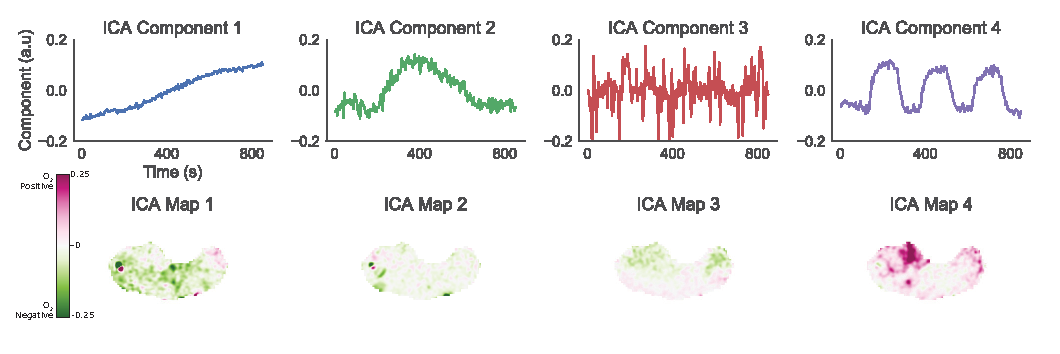
\includegraphics[width=0.9\textwidth]{oemri/oemri-images/fig_components.pdf} % requires the graphicx package
   \caption{Plots of the four components extracted from ICA are shown (($||c_i||=1, \forall i $) along with the corresponding  weighting factor maps (normalized to mean voxel wise mean signal intensity). Note that c$_4$ is clearly the component of interest here as the cycling pattern is not present in any other component. We speculate that c$_1$ corresponds to a temperature drift over the course of the scan and c$_3$ is likely related to a breathing motion artefact. Component 2 is a relatively weak spurious signal fairly low in magnitude with no obvious spatial or temporal pattern. Further investigation is required to explore the underlying physiological response (if any) of the other components.
   \label{Sfig_components}}
\end{figure}



% ======================================================================
\section{Conclusions}
% ======================================================================
In this study we extend existing oxygen-enhanced MRI techniques by adding a cycling element to the respiratory challenge and using a blind-source separation signal processing technique (ICA) to extract the oxygen responsive component and responding voxels.
This dOE-MRI method presents significant improvements to the sensitivity and applicability of OE-MRI where small changes in T$_1$W signal intensity arising from cycling respiratory challenges can be separated robustly. Traditional quantitative T$_1$ mapping techniques have longer imaging times and are impractical for OE-MRI due to SNR and time constraints.
dOE-MRI with ICA is clinically translatable as the sequence acquisition is relatively short and most centers already have access to dynamic T$_1$W MRI acquisitions that many patients already routinely receive. 
Therefore dOE-MRI is an exciting, non-invasive and widely available technique for assessing tumor oxygenation that could provide a crucial tool in the field of radiation oncology and in the development of treatments targeting the tumor microenvironment.

% ======================================================================
\section{Acknowledgments}
% ======================================================================

Dr. Martin McKeown provided assistance in understanding the utility of ICA in the given context. Dr. Alastair Kyle undertook foundational work by designing and building the microscope and histology acquisition system. 


\endinput

\section{Supporting Information}

Additional Supporting Information may be found in the online version of this article.

\textbf{Supporting Information Figure S1}. Plots of the four components extracted from ICA are shown (($||c_i||=1, \forall i $) along with the corresponding  weighting factor maps (normalized to mean voxel wise mean signal intensity). Note that c$_4$ is clearly the component of interest here as the cycling pattern is not present in any other component. We speculate that c$_1$ corresponds to a temperature drift over the course of the scan and c$_3$ is likely related to a breathing motion artefact. Component 2 is a relatively weak spurious signal fairly low in magnitude with no obvious spatial or temporal pattern. Further investigation is required to explore the underlying physiological response (if any) of the other components.

%% The following is a directive for TeXShop to indicate the main file
%%!TEX root = ../diss.tex

\chapter{Chemical Exchange Saturation Transfer}
\label{ch:CEST}

\section{Preface}

\section{Introduction}

In the year 2000, Ward, Aletras, and Balaban published a seminal paper describing a new phenomenon called chemical exchange saturation transfer (CEST).
In fact, this effect had actually been used in MR spectroscopy for over 40 years before this discovery but under a slightly different name: magnetization or saturation transfer.
Since Ward et al.
published their exciting results using exogenous agents to enhance the CEST affect, CEST-MRI has garnered significant attention as a method of generating contrast \emph{in vivo}~\cite{Sherry:2008jg}.
The CEST effect arises when magnetization is transferred through protons, between a saturated pool and an unsaturated pool.

\section{Theory}

In the context of conventional MR spectroscopy, chemical exchange occurs between protons on different chemical species and the exchange process is governed by basic forward and reverse rate constants.
Consider a system with two distinct pools of protons are able to undergo chemically exchange, for example protons from the surrounding water (Pool A) capable of exchanging with a proton on a molecule (Pool B).
Recall that when a spin $\frac{1}{2}$ particle (for e.g., a proton) is placed in a magnetic field, two possible energy states are possible (Fig~\ref{saturation}), one aligned with the magnetic field (low energy) and one aligned against the magnetic field (high energy).
The spins aligned with the magnetic field are in a lower energy state and thus, the probability of finding the nucleus in this state is slightly higher.
The probability of a spin aligned with (or against) the magnetic field is inversely related to the energy of the  state described by the Boltzmann distribution,

\begin{equation*}
P(E\uparrow) = Ce^{\frac{-E\uparrow}{k_b T}}
\end{equation*}

where C is a proportionality constant, T is the temperature of the system, and $k_b$ is the Boltzmann constant.
A magnetization vector arises from an excess population of spins in the lower energy state and this is the source of MR signal.
The strength of this magnetization vector can be temporarily reduced by the application of a low-power RF pulse (known as a saturation pulse) directed at one, or both of the proton pools.
If the saturation pulse leads to an equal population of spins in both energy states, the net magnetization becomes zero and the system is `saturated'~\cite{Sherry:2008jg}.
However, due to ongoing chemical exchange, both the high and low energy spins from the saturated pool transfer to the unsaturated pool (Fig~\ref{saturation}).
The exchange processes describing the transfer of spins between 1) the high energy spins in Pool A and B and 2) low energy spins in Pool A and B are modelled as two independent equilibria with a rate constant governing each process separately~\cite{Woods:2006cq}.
If a saturation pulse is applied on resonance at Pool A, the net result of chemical exchange on this system (over time) is a reduction in the number of Pool B spins in the lower energy state and an increase in the number of Pool B spins in the higher energy state.
Ultimately, this leads to decreased signal intensity in the Pool B as well.
Together, saturation, transfer, and chemical exchange make up the CEST effect.

\begin{figure}[htbp]
\begin{center}
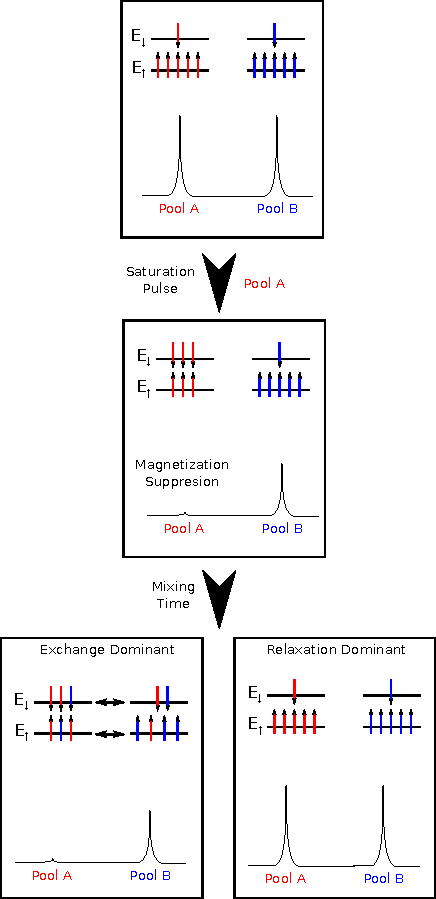
\includegraphics[width=0.4\textwidth]{cest/cest-images/cest_saturation.pdf}
\caption{\textbf{Summary of the CEST effect.} Initially two pools are considered, each with exchangeable protons.
The peaks correspond to the signal intensity from an image.
If a saturation pulse is applied with a saturation frequency at the resonance frequency of Pool A, the magnetization vector is decreased and signal intensity is suppressed.
Because of chemical exchange, the Pool B magnetization vector also decreases slightly.
If the system is dominated by relaxation (i.e.
if relaxation occurs as fast or faster than proton exchange) then the CEST effect is not observed the system recovers to its equilibrium state.
If the relaxation time is long relative to the exchange rate, a CEST effect is observed.
\newline \emph{\small{Image credit: adapted from Woods et al.~\cite{Woods:2006cq}}}}
\label{saturation}
\end{center}
\end{figure}
	
The CEST effect is only observed under specific conditions of exchange and relaxation.
At equilibrium, the spin population is distributed according to the Boltzmann distribution and the saturation pulse acts as a perturbation.
The longitudinal relaxation time (T$_1$) slowly counteracts this perturbation and if T$_1$ is short relative to the exchange rate (k$_{ex}$ describing proton transfer from Pool A to Pool B, the CEST effect is not observed~\cite{Woods:2006cq} and the system is dominated by relaxation (Fig.~\ref{saturation}).
A further criteria is that the exchange process must be slow relative to the NMR time scale,
	
	\begin{equation}
		\Delta \omega \geq k_{eq}
	\end{equation}

where $\Delta \omega$ is the difference between the Larmor frequencies of the two pools.
By saturating the bulk/free water pool, the magnetization from this pool is decreased and by saturation transfer, magnetization from the other pool also decreases.
From an imagine perspective, the net result is an overall darkening coupled with an increase in contrast as the difference between the two pools is increased.
Typically, negative contrast is not preferred in MR imaging because the human eye can more easily discriminate between a slight increase in image intensity than a similar decrease.
However, generation of this contrast can easily be controlled by turning off the saturation pulse prior to imaging.
Thus, data can be acquired with and without saturation, and post-processing techniques can be used to generate a `difference-image' consisting of positive contrast.

\subsection{APT-CEST}     

While there are several types of CEST contrasts available, in this
work we will focus our attention just on one subset, amide proton transfer or APT.
APT refers specifically to the chemical exchange between bulk-water protons and amide groups (-NH) of endogenous mobile peptides and proteins as it is most relevant for tumours~\cite{Togao:2013gn}.
The concentration of these mobile peptides and proteins is in the millimolar range and that has thusfar limited their utility to be considered a viable target for clinical diagnosis or prognosis, at least using MRI.
However due to the saturation transfer effect, APT imaging can be used to elucidate the presence of these mobile peptides and proteins~\cite{Zhou:2003cc}.
The APT effect arises when the amide groups on the protein backbones exchange with water protons after a saturation pulse directed at around 3.5 ppm with respect to water~\cite{vanZijl:2003in}.
Interestingly, the side chains of these same proteins and peptides comprising mostly the amino acids glutamine and asparagine that
resonate at about 2 ppm~\cite{vanZijl:2003in}.
Another potential contribution to the APT effect are the nucleosides that make up DNA and RNA molecules (nucleotides - adenosine, guanine, cytosine, uracil, thymine -  just without a phosphate group) but in their normal forms, the base pairs are hydrogen bonded so the exchange rates of those protons is very low (k$_{ex}$ < 0.01 s$^{-1}$) and these protons exchange very slowly with water.
When these DNA and RNA base pairs are caused to break down, denature, or separate, the labile protons are exposed and the concentration of exchageable protons increases resulting in a higher APT signal.
One can hypothesize that a treatment resulting in direct DNA damage and protein denaturation to expose additional hydrogens that could exchange with water would result in an APT signal increase in tumours.

Recently, CEST has been proposed to assess several the efficacy of several therapies and in this study we extend this work by first assessing the baseline variability of the APT effect, and then evaluate the efficacy of two treatments that may result in DNA damage (10Gy dose of whole-body radiation), as well as rapid loss of perfusion ultimately resulting in large-scale tumour necrosis (chemotherapy combretastatin)~\cite{Maxwell:2002da}.
Combretastatin is a a vascular targeting drug Combretastatin A-4 phosphate (CA4P) that has been shown to have both a strong acute effect at low dose, and a long term effect at high dose~\cite{Maxwell:2002da}.
To study the effect of these treatments on the APT CEST signal, an experiment was conducted to first assess the baseline repeatability (test-retest on subsequent days) of the APT CEST signal, followed by a treatment prior to the last imaging session.

\section{Development}

\subsection{MR Sequences}

\subsection{Phantom Work}

\subsection{Quantification \& Fitting}

\section{Methods}

\subsection{Animals}: NOD/SCID mice were implanted with a murine squamous cell carcinoma (SCCVII) on the left flank and tumours were allowed to grow until they reached 500mm$^3$.


\subsubsection{Experiment 1: CEST Controls + CA4P (CestS1)}

Animals were imaged daily for three days.
Then, 7 of those mice were injected i.p.
with 120$\mu$L of CA4P at a dose~\cite{Maxwell:2002da} of 80 mg/kg and imaged 24 hrs later.


\subsubsection{Experiment 2: CEST + 10Gy (CestS)}

5 mice received a 10Gy dose of radiation and were imaged 96 hours later (CestS2).


\subsubsection{Experiment 3: CEST + 40Gy (CestS3)}

5 mice received 40Gy dose of radiation and imaged 

Wednesday November 16, 2016 5 mice were irradiated with 40Gy but left at BCCRC for monitoring.
Mice were imaged and euthanized on Nov.
22nd, 2016.

\subsection{Imaging}

Imaging was performed using a 7T small animal scanner.
CEST scans were acquired using an EPI-based imaging scheme and continuous-wave saturation with B$_1$=1.0$\mu$T for 10s at each saturation frequency offset.
Spatial resolution of the CEST scan was 0.5 mm in-plane with a 1.5 mm slice thickness.
80 offset frequencies were acquired ranging from -20 to +20 ppm with a higher spectral resolution near peaks of interest.
Total scan time for the CEST sequence was 27 minutes.

\subsection{Histology}

\textbf{Histology:} Following the last imaging session, animals were injected with 50$\mu$L of the perfusion dye carbocyanine 5 minutes prior to sacrifice and the tumours were immediately excised and frozen.
Sequential sections 10$\mu$m thick were obtained every 0.5 mm and analysed to identify the fraction of perfused vessels and necrosis.
Sections were stained with TUNEL/CASPASE to mark apoptosis and CD31 to mark blood vessels.


\section{Results}

Figures~\ref{mainCest} \&~\ref{cestFractions} summarize the main results of the study, and the conclusions are summarized here:

\begin{enumerate}
\item While some changes in a subset of tumours can be observed in Figure~\ref{mainCest}, the tumour pixel distributions in the control groups are not statistically significantly different from the CA4P treatment group (red)

\item Histological evidence also did not point to a strong effect of treatment compared to the control groups~\ref{cestFractions}

\item Consequently, comparisons of the amine and amide peak sizes to histological fraction did not yield any conclusive correlations.

\end{enumerate}

\begin{figure}[htbp]
\begin{center}
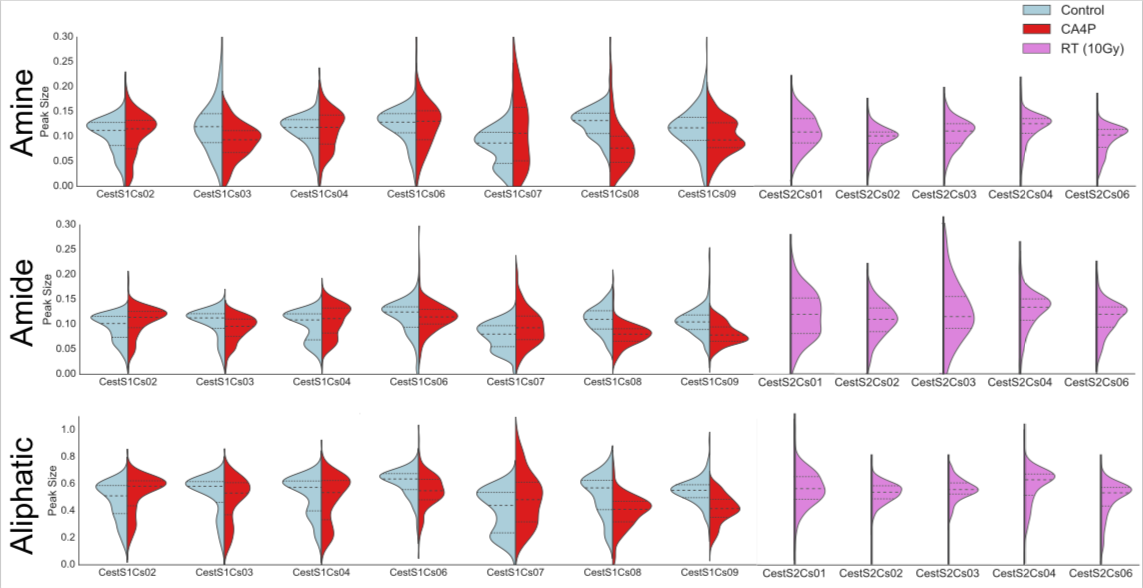
\includegraphics[width=\textwidth]{cest/cest-images/cest_Violinplots.png}
\caption{Peak-size (width x amplitude of peak) voxel distributions of every animal are shown as violin-plots for each of the three peaks of interest (amine at $\approx$2.2 ppm, amide at $\approx$3.5 ppm, and aliphatic at -3.5 ppm).
Colours represent the distribution at each treatment group: control (light blue), 24h post CA4P treatment (red), and 96h post 10Gy RT (violet).
Dashed lines within each half-violin corresponds to the median, and the dotted lines indicate the first and third quartiles.}
\label{mainCest}
\end{center}
\end{figure}

\begin{figure}[htbp]
\begin{center}
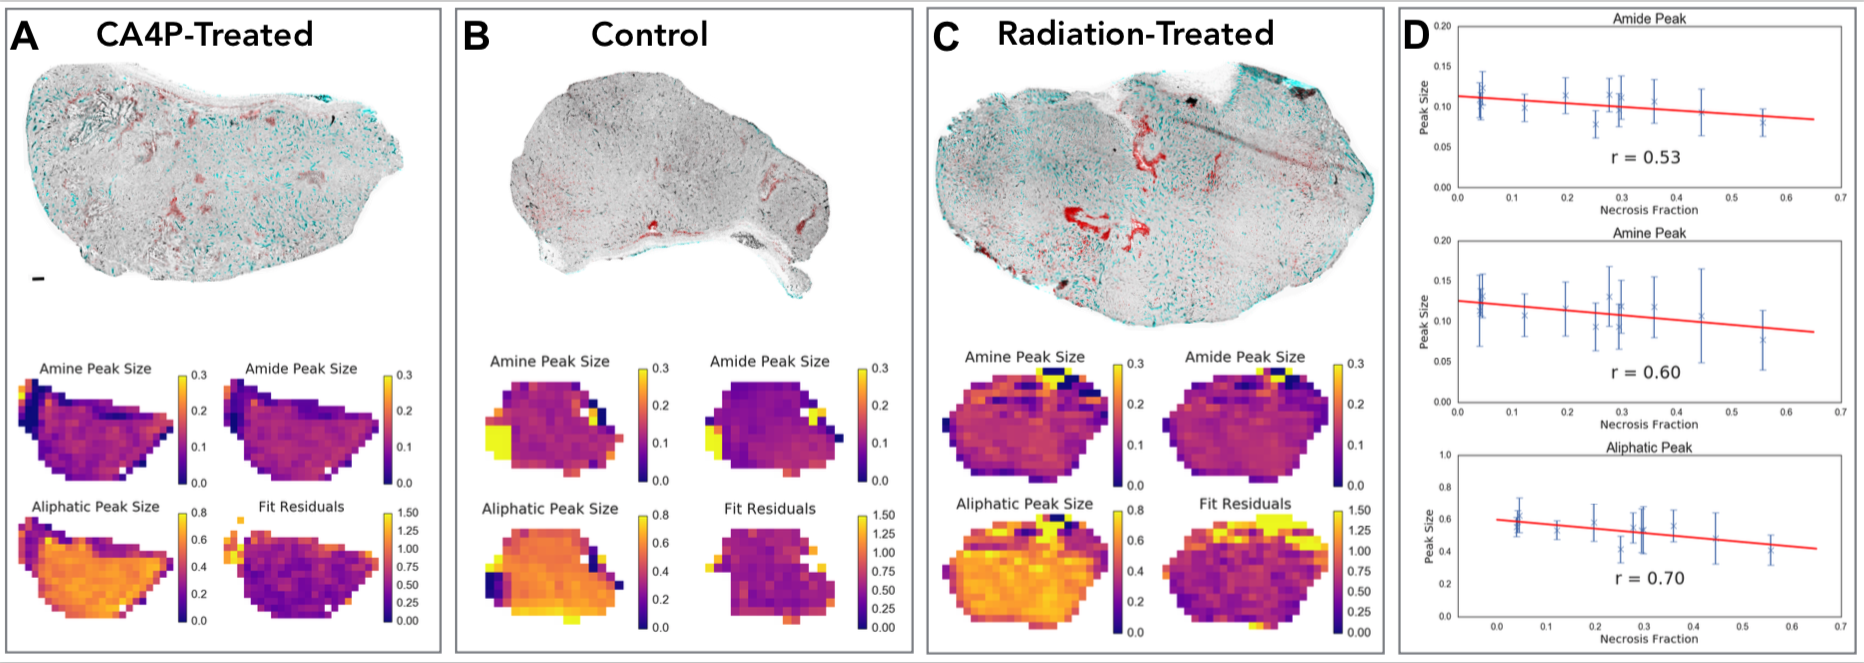
\includegraphics[width=\textwidth]{cest/cest-images/cest_RTstudy}
\caption{Representative histology sections are shown for each of the groups (A-C), as well as CEST parameter maps of a similar slice in the tumour.
CEST peak-size maps are shown for the amine, amide, aliphatic peaks as well as the fit residuals for each of the three groups.
The `fit-residual' maps were used to exclude voxels where fit quality was poor.
Necrosis fractions were calculated from the histology sections across all animals and treatment groups and plotted against the amine, amide, and aliphatic peak-sizes; r-values on the plots indicate the correlation coefficient.}
\label{cestFractions}
\end{center}
\end{figure}

%\section{Discussion}

%\section{Conclusions}


\endinput

Any text after an \endinput is ignored.
You could put scraps here or things in progress.

%% The following is a directive for TeXShop to indicate the main file
%%!TEX root =../diss.tex

\chapter{Putting it all together}
\label{ch:meltingpot}

\section{Study 1: OEMRI \& HPG}


\section{Study 2: OEMRI and HPG and CEST} 

\endinput


%\include{discussion}
%\include{conclusions}

%    3. Notes
%    4. Footnotes

%    5. Bibliography
\begin{singlespace}
\raggedright
\bibliographystyle{vancouver}
\bibliography{diss}
\end{singlespace}

\appendix
%    6. Appendices (including copies of all required UBC Research
%       Ethics Board's Certificates of Approval)
%\include{reb-coa}	% pdfpages is useful here
\chapter{Supporting Materials}

This would be any supporting material not central to the dissertation.
For example:
\begin{itemize}
\item additional details of methodology and/or data;
\item diagrams of specialized equipment developed.;
\item copies of questionnaires and survey instruments.
\end{itemize}


\backmatter
%    7. Index
% See the makeindex package: the following page provides a quick overview
% <http://www.image.ufl.edu/help/latex/latex_indexes.shtml>


\end{document}
